\documentclass[12pt, oneside]{extbook}

\usepackage{geometry}
\usepackage{listings}
\usepackage{graphicx}

\geometry{
	a4paper,
	top = 2cm,
	left = 2cm,
	right = 2cm,
}

\title{Malware Analysis}


\begin{document}
\maketitle
\tableofcontents
\chapter{Lezione 1}
\section{Introduzione alla RCE}
Reverse Code Engineering del malware, quando si analizza il malware bisogna ricostruire quello che fa a partire dal codice macchina: programma eseguibile o anche un frammento di codice macchina. La pratica di risalire da un frammento di codice al codice sorgente è il RCE.
\subsection{Definizione di Reverse Engineering}
Per definizione, per RE si definisce il processo di estrazione della conoscenza e degli schemi di progetto di qualunque oggetto costruito dall'uomo. È una attività già formalizzata nell'800, quinid ben definita già da molto tempo.\\ Un modo per capire come funziona l'attività del RE è di accostarla alla ricerca scientifica:
\begin{itemize}
\item il ricercatore scientifico accumula dei dati quantitativi, che non sono sufficienti. Bisogna estrarvi una conoscenza più astratta della realtà che c'è dietro e derivare un modello formale che rappresenti in modo formale la realtà che c'è dietro. Dall'insieme e dalle osservabili non è immediato derivare il modello formale, il processo è difficile e richiede intuizione, creatività: non basta leggere i dati, il modello va inventato. La stessa cosa vale per chi fa RE: il lavoro non è di tipo meccanico.
\item si usano opportune metodologie, altrimenti non ci sarebbe certezza che la teoria che si sta costruendo è sensata e può ragionevolmente spiegare i dati che si stanno osservando
\end{itemize}
I due grandi pilastri sono 	quindi intuizione e metodo.\\ La più grande differenza è che la ricerca investiga fenomeni naturali, mentre chi fa RE si concentra su gli artefatti umani: il ricercatore scientifico può fare delle ipotesi che non vengano semplicemente spiegate dal cervello, che ha dei limiti dal punto di vista dei modelli che può elaborare. Il ricercatore scientifico non ha certezza di trovare una teoria ed una forma a cosa sta osservando, mentre per chi fa RE c'è questo vantaggio. Quindi, concretamente c'è la garanzia che questa conoscenza era posseduta da qualcuno e che può essere riscoperta. 
\subsection{Reverse Code Engineering}
È il processo di ricostruzione delle finalità, degli algoritmi, delle strutture dati implementate da un programma per un calcolatore elettronico.\\ Ricordiamo che, con calcolatore elettronico si intende un qualunque dispositivo programmabile, non per forza un PC o laptop. Ci sono vari modi di riferirsi al RCE, come de-compilazione, ingegneria inversa dei programmi, in generale si parla di reversing.\\ Vedendo il reversing come una black box, l'input del RCE è una rappresentazione "a basso livello" del programma per il calcolatore, come ad esempio il file eseguibile contenente il codice macchina. L'output può essere variegato: è una rappresentazione a più alto livello, ma non possiamo dire con esattezza cosa debba esser in quanto quando si fa reversing non c'è un singolo use case:
\begin{itemize}
\item conoscere gli effetti del programma, allora l'output è la descrizione degli effetti del programma
\item voglio esaminare il protocollo di comunicazione, otteniamo la descrizione del protocollo
\item etc...
\end{itemize}
Si passa sempre da un livello di bassa comprensione ad uno più altro.\\ Ma alto e basso sono relativi, quindi occorre capire e definire cosa si intende per alto e basso livello.
\subsubsection{Motivazioni del reversing}
Cerchiamo di capire perché si fa reversing, non tutte le motivazioni hanno lo stesso livello etico o valore legale. Alcuni casi di utilizzo:
\begin{itemize}
\item abbiamo scritto un programma perdendo i sorgenti. Facciamo il reversing del programma per capire cosa faceva, questo è lecito. Se il programma è dell'azienda ed ho il consenso è lecito. È una attività che spesso si usa per programmi legacy in azienda.
\item programma di terzi, commerciale, che deve interagire con un altro programma scritto da noi. Vogliamo fare in modo che i due programmi si interfaccino bene, può essere necessario fare reversing sul programma per vedere come integrarlo meglio. Se è lecito o no dipende da licenze e legislazioni del paese
\item programma scritti da terzi, facciamo reversing per capire come rendere un programma simile più efficiente e compatto. È ancora meno lecito del caso precedente, tipicamente l'altra parte può dire che il lavoro viene sfruttato per avere vantaggi
\item siamo in una azienda che tiene alla sicurezza dei dati, per l'azienda è un problema affidarsi a programmi di 3° parti. Come fa l'azienda a fidarsi che non vengano esfiltrati i dati dai dischi da parte del programma utilizzato? Uno dei modi per verificare che sia tutto apposto è fare il reversing dell'applicazione. Sembra lecito, ma tutte le licenze dei programmi commerciali la vietano, quindi a rigore non si può fare
\item superare i meccanismi di protezione digitale, se c'è un sistema di protezione e si fa il reversing si sta commettendo un atto illegale.
\end{itemize}
Si fa reversing per analizzare il comportamento del malware per analizzarne gli effetti, o per produrre delle forme di protezione verso di essi come gli antivirus: gli antivirus sfruttano due grandi tecniche per il funzionamento
\begin{enumerate}
\item riconoscere la firma del virus
\item riconoscere una sequenza di operazioni "tipiche" fatte dai virus 
\end{enumerate}
il problema è fare il reversing dei virus in circolazione per poter costruire l'antivirus.\\ Si può fare reversing del malware anche per scrivere nuovi malware, in modo da cambiare le firme ed esulare gli anti-virus appena diffuso\\ Un'altra attività di reversing viene fatta sui SO, al fine di attaccarli ad esempio tramite 0-day (ovvero attaccare con dei malware mai visti prima), o anche per rendere il SO più robusto.\\ C'è poi un'area del reversing che si occupa delle debolezze degli algoritmi crittografici, nella loro implementazione.\\ Alcune di queste attività sono illegali, alcune addirittura in quasi tutte le nazioni del mondo. Ci sono attività  legali o tollerate, perché il punto chiave è il perché si fa questa attività ad esempio a scopri di didattica, anche se fatto su programmi commerciali. Anche se nelle licenze d'uso c'è scritto che non è possibile fare RCE, questo può essere vessatorio, quindi poi la decisione finale spetta al sistema giuridico. \textbf{esempio:} sembra essere consentito in Italia fare reversing sul software di una stampante al fine di vendere cartucce di inchiostro riciclate. Le stampanti bruciano dei bit del componente elettronico della cartuccia quando questa è terminata, quindi occorre capire come questo viene fatto dal software.\\ La cosa diviene illegale se io faccio la stessa cosa per vendere cartucce nuove compatibili con la stampante.\\ L'attività ed i tool sono sempre gli stessi, ma quello che cambia è \textbf{il perché} viene fatta: spesso il confine fra legalità ed illegalità è sottile. L'attività di RCE non è lecita o illecita di per se, è lo scopo che se ne fa che la rende tale (Ricorda la differenza fatta a SERT fra hacker e cracker).
\subsubsection{Principi generali del RCE}
IL RCE può essere considerato l'operazione inversa della programmazione: nella programmazione l'idea di algoritmo viene tradotto in linguaggio di alto livello e poi compilato in codice macchina; in RCE si fa l'opposto.\\ Un programmatore segue dei principi nello scrivere il codice, quanto più si adottano correttamente i principi, quanto più si fa bene. Anche nel RCE vanno seguiti una serie di principi e regole generali per fare un buon lavoro. I principi generali:
\begin{itemize}
\item[\#] \textbf{Maggiore è la comprensione dell'interno sistema, tanto più rapida ed efficiente è l'attività di reversing}. Non si può fare reversing di qualcosa di qui non si sa nulla, l'hacker che fa il reversing deve essere competente in diversi settori dell'informatica: SO, architetture dei calcolatori, etc... Meno cose si sanno, più difficoltà si avrà nel lavoro di reversing. Altre competenze da avere è capire il processo di compilazione del programma, come i costrutti di alto livello vengono tradotti in assembly, siccome i dettagli dipendono dal compilatore cambiano a seconda del compilatore. Il formato del file eseguibile è un altro elemento importante: una cosa sono le istruzioni macchina, un altro è il contesto di esecuzione del file eseguibile, ovvero di come poi il programma verrà effettivamente eseguito. Inoltre, il lavoro di reversing è una "battaglia di teste" e siccome chi ha scritto il malware non ha interesse che sia analizzato, mette in piedi una serie di misure di offuscamento, protezione, rilevazione del debugger, in macchine virtuali e sandbox e altro. Chi fa il malware vuole proteggersi da chi vuole analizzarlo, inventando sempre nuove soluzioni ed il lavoro è cercare di capire e superare queste soluzioni.\\ Per questo motivo, fare reversing è sempre un atto creativo, dove si usa sempre la testa ma va comunque supportato dalla conoscenza e quindi richiede un continuo sforzo ed aggiornamento.
\item[\#] \textbf{Per capire il codice scritto da alti, è necessario capire come funziona il proprio}. Se chi ha scritto il malware ha necessario, ad un certo punto, una struttura di dati dinamica, come un albero bilanciato, è necessario sapere come gestire e implementare una struttura dati dinamica. L'obiettivo del processo di reversing non è capire cosa fa una singola istruzione macchina, bensì tutto ciò che fa il programma per capire cosa pensava chi l'ha concepito. È essenziale saper programmare bene
\item[\#] \textbf{L'attualità e la conoscenza dei tool di reversing determina la qualità del processo di reversing}. Le applicazioni moderne sono costituite da una grande quantità di codice macchina, che non è gestibile a mano. Ormai sono sempre più grandi di ciò che si può gestire senza strumenti sofisticati, quindi bisogna saper usare gli strumenti giusti. Oggi, ghidra è uno dei principali strumenti per fare RCE (open source). Gli strumenti sono sofisticati, la curva di apprendimento non è del tutto lineare, per cui è necessaria molta pratica per saperli usare.
\item[\#] \textbf{La chiave del reversing è la capacità di identificare e comprendere gli schemi ricorrenti nel codice, di conseguenza non esiste sostituto dell'esperienza}. La bravura di chi fa RCE si misura nel numero di ore dedicate al fare reversing. È sempre un principio generale, tanto più si ha esperienza, quanto più è rapido fare RCE.\\ I compilatori producono i costrutti di alto livello in certi pattern di codice macchina, con i decompiler si ottengono i pattern ad alto livello ma non è detto che il codice ad alto livello sia più facile da capire cosa il programma fa dal codice ad alto livello. L'abilità principale dell'hacker esperto è quella di saper riconoscere le strutture nascoste nel linguaggio macchina
\end{itemize} 
I principi generali di per se non sono sufficienti, serve anche metodologia. Alle volte si dice che la programmazione è arte, compresa solo da altri programmatori. In effetti, anche l'attività di RCE può essere considerata una forma d'arte perché richiede intuizione, capacità di problem solving. Punto importante: metodo, costanza, tempo e impegno mettono in condizione chiunque di poter fare questo mestiere.
\subsubsection{Metodologia}
Non si può prescindere dalla metodologia, bisogna avere ben chiari gli obiettivi. Bisogna avere chiaro la domanda a cui dare risposta e deve essere chiara, perché se ci cerca di scoprire tutto, può richiedere moltissimo tempo. Occorre stabilire in che modo ottenere l'obiettivo: se c'è un virus pericolo che può infettare la macchina, non c'è cosa più pericolosa di essere infettati sulla macchina con cui si fa reversing: non deve mai avvenire, quindi non è detto che si può operare sul malware eseguendolo. Inoltre, essendo un processo creativo, bisogna di continuo verificare la correttezza di cosa si sta facendo. Tutto ciò rende necessario formalizzare una metodologia, meglio se scritta. Gli approcci fondamentali del reversing:
\begin{itemize}
\item analisi "black box" o live code analysis: eseguo il programma e cerco di capire cosa fa, in ambienti più o meno controllati. Non è sempre possibile farlo e non può fornire informazioni su porzioni di codice non eseguite
\item analisi white box: analizzo il codice e cerco di capire cose fa "guardando nella scatola". Il problema dell'analisi è il costo in termini di effort e di tempo
\item analisi mista o gray box: approccio che in linea di principio combina metodi white box e black box, mischiando i due livelli. Il principale tool che si usa in questa fase è il debugger, in generale la metodologia è molto efficace e quindi nei malware ci sono una serie di elementi per cercare di renderla difficile.
\end{itemize}
Esempio di metodologia generale in 9 passi:
\begin{enumerate}
\item descrizione preliminare: descrivere cosa si sa, da dove viene il malware, cosa ha prodotto etc... Tutto quello che si sa va scritto
\item formalizzazione dell'obiettivo: non possiamo pensare di sapere tutto. Decidere cosa scoprire, ad esempio l'IP a cui si collegava, che file ha esfiltrato. Passo cruciale, perché l'attività di reversing va centrata su questo passo, inoltre permette di definire quanto tempo ci metterò a fare reversing
\item ottenimento del codice macchina: può essere immediato, alle volte il codice è offuscato o protetto con cifratura. È un passo non banale, alle volte è necessario fare il de-offuscamento a mano
\item osservazione del funzionamento: se posso, faccio analisi black box, è analisi dinamica. In alcuni casi non posso farla, se il codice ad esempio sfugge al controllo o se non posso eseguirlo
\item disassemblaggio white box, se non ho risolto il problema al passo 4, tipicamente si usano disassemblatori interattivi, ovvero che consentono di interagirvi per indirizzarlo nel suo lavoro. Può non funzionare correttamente, perché sono state usate delle contro misure
\item localizzazione del frammento assembly: trovo il frammento che può rispondere alla domanda. Servono delle tecniche per trovare il punto di interesse. Sono varie le tecniche per fare il passo
\item analisi del frammento assembly: una volta trovato il punto, si cerca di comprenderlo. È la fase più critica, è necessario ed essenziale annotare tutto ciò che si trova e se durante la fase ci sono punti che tornano ad essere interessanti si reiterano i precedenti punti
\item verifica dei risultati: occorre verificare che quanto scoperto è corretto
\item riepilogo in un report: viene riepilogato tutto ciò che è stato fatto, cosa si è appreso, cosa si è ottenuto etc...
\end{enumerate}
\section{Concetti fondamentali di analisi del malware}
Per fare analisi del malware, ci sono due grandi possibilità per quanto riguarda i sistemi host:
\begin{itemize}
\item Linux
\item Windows
\end{itemize}
La nostra attività di reversing è focalizzata sull'analisi del malware e questo attacca nella maggior parte dei casi sistemi Windows, ma la scelta di usare Windows come sistema per analizzare il malware non è per forza la migliore: su Linux non è possibile eseguire il malware per natura, quindi si evitano eventuali pericoli di esecuzione del malware sulla macchina host.\\ Non vuol dire che non esistono malware per Linux, ma sono rari ed a quel punto è possibile analizzarli spostandosi in ambienti Windows. D'altra parte, è comodo avere anche degli ambienti che esegua in maniera controllata il malware: se il sw è Windows-based, serve anche un ambiente Windows. Si può quindi usare come base un host Linux ed avere Windows come VM:
\begin{itemize}
\item è possibile scegliere la versione di Windows più adatta da installare sulla VM, magari per far girare dei malware patchati da determinate versioni di Win (ne usiamo quindi una vulnerabile)
\item l'host viene usato per l'analisi, mentre la VM per l'esecuzione
\end{itemize}
Possono esserci diverse scelte come VM per il reversing:
\begin{itemize}
\item VmWare, molto usata per il reversing
\item VirtualBox
\item QEmu, rispetto alle prime due, questa è disponibile solo per Linux
\end{itemize}
Il vantaggio della VM è che è possibile costruire degli snapshot: se viene perso il controllo e la macchina è infettata, è possibile ripristinare lo snapshot per riparare al danno.\\ È possibile (teoricamente) che il malware si diffonda da una VM Windows al sistema host sempre Windows: tipicamente un malware ha delle contromisure per capire se sono in esecuzione sulla VM o sul sistema host. È necessario da parte dell'analista capire come fa il malware a vedere che è in esecuzione su una VM ed inibirlo. Il malware può fare un numero limitato di controlli, il grande vantaggio di chi fa l'analisi è che avendo il controllo sul codice può patcharlo e farlo eseguire sotto specifiche condizioni.\\ Ci sono comuqnue dei casi in cui è possibile che si riesca ad infettare il sistema host dalla VM, ma in ogni caso l'esecuzione in VM è un grande passo avanti di sicurezza. Inoltre, può accadere che l'antivirus presente nella versione di Windows abbia un anti-virus per-installato che magari blocca il malware, quindi andrebbe disabilitato per un tempo limitato per evitare che ciò accada.
\subsection{Come fare RCE}
Possiamo vedere il RCE come una scatola nera, in cui entra codice macchina ed esce una rappresentazione di alto livello che vogliamo ottenere dall'analisi. Il problema sta proprio nel codice macchina, per poter fare reversing occorre capire come è fatto e da dove viene fuori.\\ Il codice macchina è generato nel processo di compilazione:
\begin{itemize}
\item la compilazione parte dal file sorgente
\item i primi componenti che processano il file sono il \textbf{pre-compilatore}. Ad esempio, in C esiste la direttiva \textsf{include}, o definire le macro, il pre-compilatore si occupa di aggiungere gli include e sostituire le macro nel file. Il risulato passa ad un secondo parser chiamato \textbf{compilatore}
\item l'output della comilazione è il file oggetto, che non è un programma eseguibile, che contiene le istruzioni macchina corrispondenti al programma nel file sorgente. 
\item Questo meccanismo viene ripetuto per ognuno dei file sorgente, tutti i file oggetto finiscono al \textbf{linker}, il risultato è un eseguibile.
\end{itemize}
La differenza fondamentale fra file oggetto ed eseguibili sono i riferimenti: nei file oggetto, tutti i riferimenti ai file sorgente sono appesi, ad esempio le chiamate alle funzioni di libreiria. Non si possono risolvere, il linker mette assieme il contenuto dei file oggetto. Ad esempio, mettere a posto i riferimenti tra diversi file sorgente o le librerie.\\ Nelle librerie ci sono una serie di funzioni già pronte che vanno collegate al file sorgente (es: printf, scanf etc...) ed è il linker a predisporre il collegamento.\\ Il file eseguibile non contiene solo le istruzioni dei file sorgente e delle librerie, ma anche concetti relativamente al processo (vedi meglio); inoltre c'è differenza fra librerie statiche e dinamiche:
\begin{itemize}
\item nelle librerie statiche, ogni volta che serve una funzione, si cerca nell'opportuno file il codice che realizza la funzione e viene copiato nel file eseguibile il codice macchina necessario
\item nel collegamento dinamico, il linker registra nell eseguibile che una certa funzione verrà fornita a run time dal SO, ad esempio le dll di Windows o shared object di Linux. Quindi, alla "creazione del processo" verrà fornito il codice da eseguire
\end{itemize}
Nell'analisi del malware, le librerie dinamiche sono un vantaggio da un certo punto di vista ed uno svantaggio da un altro lato: non è banale capire cosa fa del codice, se è linkato staticamente magari è una banalità ma essendo linkato staticamente è difficile capire cosa fa. Se la libreria è dinamica ed il malware fa riferimento alla funzione, capisco dal nome cosa fa la funzione. In generale è un vantaggio se il malware usa librerie dinamiche, anche perché tipicamente l'eseguibile risultante è più piccolo se ci sono librerie dinamiche. È uno svntaggio se chi fa l'analisi del malware non riesce a capire quali sono le librerie dinamiche che il malware usa e questo può diventare un problema.\\ Quindi, non c'è una risposta esatta: entrambe le opzioni hanno vantaggi e svantaggi.\\ Abbiamo quindi del codice macchina, a questo punto va analizzato
\begin{itemize}
\item l'analisi statica cerca di prendere il codice e capire cosa fa, ci sono due grandi tool per fare questo lavoro
\begin{itemize}
\item disassemblatore, che possono essere
\begin{itemize}
\item lineari, ovvero un tool poco complesso da capire e da utilizzare. Va bene per piccoli malware ma diventa più difficile fare dei lavori più complessi. Esempi: objdump di Linux\\ Nell'architettura dei calcolatori (di Von Neumann), i dati ed i programmi sono memorizzati nella stessa memoria, quindi l'eseguibile ha sia dati che istruzioni macchina. Se trovo un byte "103", come lo interpreto? È un dato, una variabile pari a 103? Non c'è modo di capire cosa sia, e questa è la grande differenza fra i disassemblatori lineari e quelli interattivi: il disassemblatore lineare parte dalla prima istruzione macchina che viene eseguita quando si lancia il programma e da lì scende, andando per sezioni. Se nel processo c'è un salto nel codice e in mezzo ci sono stringhe o altro, il disassemblatore va avanti e continua ad analizzare quel codice come se fossero istruzioni macchina.
\item interattivi: ad esempio Ghidra ed IdaPro (di cui esiste una versione gratuita, ma sta bene dove sta). Il disassemblatore interattivo parte dall'entry point del programma e segue il flusso: dove trova un salto, sa che c'è codice, se trova una chiamata a funzione c'è codice. Dovunque non arriva, lascia in incognito. È interattivo perché è l'analista a dire che in determinati punti c'è codice per far si che il disassemblatore conitnui, questo implica un uso corretto del tool, fornendo informazioni all'interno di essi.
\end{itemize}
\end{itemize}
\end{itemize}
Quando viene costruito un file oggetto o un esegubile, viene organizzato in modo da riconsocere le informazioni: un file oggetto ha un certo numero di sezioni:
\begin{itemize}
\item testo: c'è il codice macchina
\item data: contiene variabili inizializzate con valore diverso da 0
\item bss: contiene la descrizione delle variabili inizializzate a 0
\item read only: dati costanti, ad esempio le stringhe esplicite
\end{itemize}
Nel file esegubile, più sezioni sono collassate in segmenti dove ogni segmento è descritto dal modo in cui il SO deve preparare le pagine che contengono i dati e le istruzioni, e potrebbero andare a finire nella stessa pagina perché devono essere pagine read only. In architettura Intel non ha quindi molto senso differenziare testo e read only, poi quando si porta in memoria ci sarà il processo per cui quando si porta in memoria ci saranno le diverse pagine corrispondenti ai segmenti.\\ Windows e Linux usano formati differenti di eseguibili:
\begin{itemize}
\item ELF per Linux
\item PE-Coff storicamente, oggi sono PE(32 bit) o PE+(64 bit)
\end{itemize}
È importante sapere del formato del file esegubile, chi scrive malware sa che chi lo analizza usa un debugger interattivo e quindi stravolge il formato del file eseguibile per evitare che chi lo analizza capisca come è organizzato il file. Quindi, provo ad usare il disassembler e quello non capisce niente (cit): magari parte dall'entry point sbagliato o altre conto misure.
\subsubsection{Eseguibili a 32 bit o 64 bit}
I processori Intel sono nati a 32 bit, ma uno dei dogmi commerciali è la compatibilità verso i programmi precedenti, quindi c'è la capacità di processori moderni di eseguire programmi a 32 bit.\\ Quindi, ogni pagina di memoria ha un bit che indica se questa ha istruzioni a 32 o 64 bit ed il processore è in grado di fare swapping fra le due dimensioni e quindi di avere SO che supportano esegubili a 32 e 64 bit. \\ Dobbiamo quindi gestire due ISA diversi, uno a 32 ed uno a 64 bit. La gran parte del malware è ancora scritta a 32 bit: se scrivo malware è perché lo voglio diffondere il più possibile, in modo da farlo girare sia su nuove che su vecchie macchine. Quindi ancora oggi gran parte del malware è a 32 bit, ma cominciano a diffondersi anche malware a 64 bit.
\subsubsection{Little endian vs Big endian}
I processori Intel sono little-endian: il byte è l'unità di base del processore, che vengono aggregati per rappresentare valori più grandi:
\begin{itemize}
\item word: 4 byte
\item quad-word: 8 byte
\item etc...
\end{itemize}
Nell'interpretazione little endian si mette all'indirizzo di memoria più piccolo il valore meno significativo del numero, mentre big endian è l'opposto. \textbf{esempio: 515} è fatto di due byte: 2 3 (2*256 + 3). Se il valore è codificato in little endian, viene rappresentato in memoria come 3,2 mente in big endian abbiamo 2,3 e può accadere che nel programma si usi un protocollo di rete e se va usato un valore va codificato in big endian, quindi il disassemblatore non lo sa e deve essere l'analista a scoprirlo.
\subsubsection{Numeri esadecimali}
Base 16, cifre da 0-9 e lettere da a-f. Importanti perché ogni cifra esadecimale è mezzo byte, quindi è immediato prendere un numero exdec e capire la maschera di bit: 515 = 0x(0)203. Ghidra usa la sintassi assembly della Intel (ufficiale dei manuali), mentre un tool come objdump usa la sintassi AT \& T. Il compilatore gcc ha una toolchain interna che usa AT \& T, quindi può capitare di dover fare reversing di codice che viene fornito con questa sintassi. La grande differenza fra le due sta nell'ordine dei parametri (src e dest), poi ci sono altre differenze minori.
\subsection{Attività di reversing}
Tentativo di apertura di un programma con Ghidra (fatti un hello world  ed aprilo).\\ Dopo l'analisi del file, ghidra elenca alcune cose iniziali:
\begin{itemize}
\item header, dove è inidicato come creare il processo una volta che il programma va in esercizio. Nell'header PE ci sono alcune tabelle, la prima delle quali non è molto interessante poiché descrive il file come se fosse dos (ma ormai i file dos non si usano più)
\item IMG\_NT\_HEADERS32: i primi patrametri della tabella sono una signature, che permette di riconoscere il file come PE.\\ Ci sono poi due tabelle principali chiamate IMG\_FILE\_HEADER ed altra, che contengono infromazioni molto importanti:
\begin{itemize}
\item architettura della macchina
\item timestamp di quando è stato costruito il file
\item address o entry point: prima cosa essenziale da capire. Accanto all'interpretazione, sono  mostrati i byte corrispondenti. Ghidra quindi assegna una label ad ogni indirizzo e questa è significativa se ha scoperto a cosa fa riferimento. Doppio click sulla label porta nel punto del file corrispondente.
\end{itemize}
\end{itemize}
La "entry" è una posizione nel file, ma anche una posizione in memoria: c'è una doppia visione di ogni cosa di cui si fa reversing
\begin{itemize}
\item visione fisica, del file esegubile
\item visione della memoria (RAM) associata al processo quando il SO esegue il file eseguibile
\end{itemize}
Queste due finestre sulla realtà vanno di pari passo: il file eseguibile è diviso in segmenti, avremo quindi dei segmenti per code, data, bss e read data e ciascuno di questi corrisponde a delle pagine di memoria usati per contenerli, avremo quindi delle pagine dedicate al codice che corripsondono alla zona del file dove ci sono le istruzioni. Un'altra parte sarà dedicata ai dati, che corrispondono però sia al segmento dati che al bss poiché le variaibli sono trattate similmente.\\ Stesso vale probabilmente (ma dipende dall'implementazione) anche i dati readonly finiscono in una zona dati, perché la protezione sulla scrittura dei dati è implementata a compile time, ma non c'è reale necessità ad imepdire che quella zona di memoria non venga scritta perché nel programma non ci sono istruzioni che le scrivono.\\ Ci sono altre almeno due zone di memoria, ovvero stack ed heap:
\begin{itemize}
\item heap: zona per l'allocazione dinamica della memoria, in modo quasi arbitrario
\item stack: zona presente in tutti i programmi, di taglia fissa e che serve per due scopi: realizzare il meccanismo di invocazione delle funzioni e correlato a questo, è usato per allcore le variaibli automatiche:
\begin{itemize}
\item variabili globali finiscono nella zona data. Visibili in tutto il programma e persistenti finché il programma gira
\item variabili locali o automatiche finiscono sullo stack, visibili sono nella procedura dove vengono definite e persistenti finché la funzione viene eseguita. Il meccanismo più comodo per allocarle è lo stack
\end{itemize}
Bisgona capire come tutto questo viene getito a livello assembler. Ci sono poi altri tipi di variabili
\begin{itemize}
\item statiche e globali: la presistenza è uguale, ma il fatto che sia statica implica che la visibilità è locale all'unità di compilazione, ovvero è visibile sono nel file dove viene dichiarata
\item statiche e automatiche: la visibilità è identica, ma la persistenza cambia, in quanto la variabile conserva il suo valore anche dopo che la funzione smette. Dove viene allocata la variabile: nei data. Lo stack cresce e decresce di continuo e contiene dati temporali. Lo heap è per allocazioni dinamiche, quindi viene messa nel blocco data perché dal punto di vista del funzionamento delle istruzioni macchina non c'è differenza fra variabili statiche e globali, la differenza sta a compile time nella visibilità 
\end{itemize}
\end{itemize}
\subsubsection{Indirizzi di memoria}
Abbiamo sempre due visioni: memoria e file eseguibile, cerchiamo però di essere più attenti: in Ghidra, accanto ad ogni costrutto c'è un valore numerico che è l'indirizzo in RAM del costrutto. Per passare dalla posizione sul file all'indirizzo in RAM ci sono diversi passaggi: il linker mette insieme una serie di file oggetto, con le loro sezioni di testo, data etc... e mette insieme tutto il materiale delle sezioni di testo in un unico segmento e comincia a calcolare gli offset delle istruzioni macchina all'interno del file. Costruisce quindi un file eseguibile che si presuppone venga caricato ad un certo indirizzo.\\ Supponiamo di avere: \textsf{l: mov eax, [h]}, a livello di Assembler lavoriamo ancora con i nomi simbolici. Sarà il linker a trasformare l in un indirizzo, e tutte le istruzioni dopo seguiranno di cosneguenza: conta quindi l'indirizzo dove verrà caricato tutto una volta che li programma va in esecuzione.\\ Prima, l'indirizzo di caricamento era fissato nel SO, inoltre programma differenti potevano andare in conflitto fra loro. Oggi è tutto risolto tramite meccanismi hardware e software, l'idea fondamentale è che quando il linker alla fine arriva a generare il codice macchina, questo è basato sugli \textbf{indirizzi logici}. Il processore Intel ha la memoria divisa in segmenti, ogni segmento contiene del codice e per far riferimento ai segmenti c'è un registro di processore apposito, \textsf{cs}. In Ghidra, noi troviamo l'offset rispetto alla base in memoria di dove è messo il segmento codice. Nel caso sopra, h è un indirizzo di un dato, che starà nel segmento dati, che in RAM è identificato da un altro registro segmento che è \textsf{ds}, quindi anche in questo caso è l'offset rispetto al segmento dati.\\ Windows, come molti altri SO moderni, non usa la segmentazione a pieno ma adotta un meccanismo flat memory: l'indirizzo di base di tutti i segmenti è 0, quindi l'offet nel codice macchina è formalmente un offet del segmento, ma è anche un identificativo univoco della memoria. (offest + 0 = offset).\\ Col modello di memoria piatto però, non si può più avere offset uguali, perché tutti partono da 0 e quindi c'è un problema: lo spazio di indirizzo delle istruzioni macchina, dello stack, dei dati etc... coincidono.\\ Ora, partendo dall'indirizzo logico, tramite l'unità di segmentazione arrivo all'indirizzo lineare che non è ancora quello finale perché c'è un altra unità hardware che è la paginazione: tramite le Page Table, è possibile tradurre l'indirizzo finale in un indirizzo fisico che viene usato nel bus per accedere ad una certa cella della RAM.\\ Di fatti, nei SO moderni i segmenti principali sono tutti a 0, quindi quello che veramente lavora è l'unità di paginazione: la funzione principale è realizzare un meccanismo di protezione della memoria:
\begin{itemize}
\item un programma viene caricato dal compilatore tipicamente ad un indirizzo prestabilito, che è un indirizzo logico
\item la paginazione fa si che ogni processo abbia delle PT differenti e che mappino su indizzi fisici differenti ovvero su celle di RAM differenti
\end{itemize}
Si parla di \textbf{indirizzi virtuali} quando il mapping fra indirizzi fisici e indirizzi lineari non è fissato ma cambia di continuo. Nel codice macchina siamo ancora a livello di indirizzo logico, e bisogna tenere presente il meccanismo che lo tradurrà in un indirizzo fisico.\\ Andando all'indirizzo indicato da "entry", si arriva ad un indirizzo (CHE È IN LITTLE ENDIAN) a cui va sommato l'offset dove viene caricato il file per ottenere l'indirizzo logico.\\ Non è detto però che quando il programma in Windows, quando lanciato, viene caricato nell'indirizzo prestabilito ma può capitare che il file sia rilocato
\subsubsection{Regstri del processore}
A 32bit, abbiamo i seguenti registri:
\begin{itemize}
\item registri general purpose
\begin{itemize}
\item eax (dove ax è a 16 bit, ah ad 8 bit e al a 4 bit)
\item ebx
\item ecx
\item edx
\end{itemize}
tutti con le contro parti a 8, 4 bit
\item altri registri
\begin{itemize}
\item esi
\item edi
\item ebp
\end{itemize}
\item registri segmento
\begin{itemize}
\item cs
\item ds
\item es
\item fs
\item gs
\item ss
\end{itemize}
\item usa serie di registri speciali
\begin{itemize}
\item esp: stack pointer
\item eflags: bit che contengono lo stato corrente del processore
\item eip: istruction pointer, non è un registro visibile direttamente, si può manipolare solo con istruzioni di salto e decisioni
\end{itemize}
\item registri per manipolare lo stato interno dei processori
\item registri per manipolare i co-processori: un tempo i componenti con registri floating point erano venduti separatamente
\begin{itemize}
\item fpr0 - fpr7 (mmx0 - mmx7)
\end{itemize}
\end{itemize} 
In realtà tutti i processori moderni hanno una ISA a 64 bit, i registri hanno anche una parte composta da 32 bit in più ad hanno la r davanti al nome. Inoltre, vengono aggiunti anche nuovi registri r8 - r15.
\subsubsection{Gestione dello stack}
Lo stack dei processori è full descending: il processore lavora a 32 bit ed ogni cella di stack è di 4 byte. Lo stack cresce dal basso verso l'altro, esp in ogni momento contiene l'indirizzo dell'ultimo elemento, ovvero di quello riempito (lo stack è LIFO) da cui si dice che è \textbf{full} perché punta all'ultimo elemento inserito. Descending perché gli indirizzi crescono mano a mano che si scende verso gli elementi più vecchi, quindi ogni volta che metto un nuovo elemento lo inserisco in un indirizzo più piccolo di quello più vecchio.
\subsection{Chiamata a funzione}
Le funzioni (sia in archiretture a 32 che a 64 bit) si appoggiano allo stack. Supponiamo di usare una certa parte dello stack e troviamo una CALL ad un certo indirizzo (o etichetta) f, cosa fa il processore: le call possono essere
\begin{itemize}
\item nello stesso segmento
\item fra segmenti differenti
\end{itemize}
il risultato pratico è che ci sono più tipi di call. In genere, vediamo quelle nello stesso segmento in quanto lo spazio di indirizzi può essere largo 4G di celle e quindi sufficienti. La CALL quindi salva l'indirizzo a cui ritornare subito dopo aver fatto la chiamata, nello stack viene quindi aggiunto l'indirizzo di ritorno h ed aggiornato esp.\\ Dopo di che, viene caricato l'indirizzo f in eip, ovvero nell'istruction pointer, quando f termina lo fa con la \textsf{ret}, che prende l'indirizzo puntato da esp, lo carica in eip e poi incrementa esp in modo che punti alla locazione che sta sotto (eseguendo quindi la pop). Se la funzione fa cose sbagliate e fa una return quando esp punta ad altro e non ad h succede qualcosa di inatteso. Le funzioni devono tenere lo stack bilanciato, quindi quando si fa la return bisogna tornare ad h, ma "giocare" con lo stack è uno dei tanti modi con cui si tenta di inibire il disassemblatore per non seguire più la logica generale.\\ Quindi, una cosa è l'idea di programmazione ad alto livello, un altra è quello che riguarda il codice macchina.
\paragraph{Funzioni di diversi tipi}
Ci sono alcuni tipi di funzioni, come ad esempio quelle di tipo "thunk", che sono di librerie dinamiche (DLL) che ad esempio usano una sola istruzione per fare una jmp ad una locazione che sarà scritta a run-time
\subsubsection{Convenzione per la chiamata a funzione}
Non c'è un unica convenzione con cui avviene il passaggio dei parametri, a seconda del SO cambiano ma anche in base ad altri fattori. Le due principali sono 
\begin{itemize}
\item convenzione del linguaggio C, ovvero cdecl
\item convezione stdcall, la modalità standard con cui il SO ed i compilatori Microsoft fanno le chiamate a funzione
\end{itemize}
\paragraph{CDECL:} andrebbe distinto fra 32 e 64 bit, a 32 bit i parametri sono passati sullo stack in ordine inverso rispetto all'ordine logico della dichiarazione della funzione (perché così poi la pop ristabilisce l'ordine). Siccome vengono fatte delle push sullo stack, questi sono dati temporanei e quindi poi vanno recuperati: questo, nella convenzione cdecl va fatto dal chiamante, quindi ci saranno le pop, ma verosimilmente si fa un \textsf{add esp, 0xc}
\paragraph{STDCALL:} identica a CDECL, tranne per il fatto che chi toglie i valori dallo stack è il chiamato. Le istruzioni Intel permetto di fare questo con la \textsf{ret 12}, ovvero toglie 12 byte e ritorna al chiamante (dopo aver ovviamente tolto l'indirizzo di ritorno e messo in eip). \\\\
%disegno
Stiamo parlando di un'architettura x86, vengono messi gli argomenti in ordine inverso e poi viene fatta la call e viene messo l'indirizzo di ritorno sullo stack, ma questo serve anche per scrivere le variabili del chiamato: le variabili automatiche non hanno dei valori iniziali, quindi viene fatta una \textsf{sub} per poter riservare alle variabili lo spazio necessario. A questo punto ESP punta alla locazione dove andrà var2 (una delle due variabili della funzione). Se però la funzione vuole leggere l'argomento 1, bisogna fare i calcoli: starà in ESP + 0xtot, dove tot è dato da cosa è stato inserito nello stack quando viene preso il chiamato. Il compilatore fa tutto automaticamente, per motivi storici i compilatori usano un registro particolare chiamato EBP, che punta al \textbf{frame} sullo stack: il frame identifica la porzione dello stack dedicata ad una specifica funzione
\subsubsection{Funzionamento di EBP}
Quando viene chiamata la funzione, viene salvato EBP nello stack (\textsf{push}), perché immaginiamo che anche la funzione chiamata abbia un registro EBP e quindi all'uscita va rimesso come era prima.\\ Quindi, la prima cosa che viene fatta dalla funzione è fare un push di EBP, ovvero mette il vecchio valore di EBP, quindi ESP punta sul valore di EBP. Si sposta poi il contenuto di ESP in EBP, ovvero adesso EBP diventa = ESP, ESP puntava su old EBP e quindi EBP punta lì. Adesso è possibile muovere ESP come si vuole, perché EBP rimane fermo in quel punto dello stack, quindi la funzione fa una AND di ESP ed un valore esadecimale 0xfffff0, che in complemento a 2 è un valore negativo e quindi fare un AND logico vuol dire azzerare gli ultimi bit e l'effetto è l'allineamento dello stack ad un multiplo di 16, in quanto non siamo sicuri che lo sia.\\ La \textsf{sub} alloca spazio nello stack di 10 ex, ovvero di 16 byte e quindi di 4 variabili, EBP rimane come prima, mentre ESP si muove e punta sull'ultima variabile allocata. Ora per identificare gli argomenti della funzione, si usa EBP:
\begin{itemize}
\item argomento 1: EBP + 8
\item argomento 2: EBP + 12
\item argomento 3: EBP + 16
\end{itemize}
Ma a questo punto ESP si può usare a piacere e modificarlo come si vuole, e si usa EBP per fare l'accesso alle variabili allocate prima, stavolta con EBP - 0xtot (RICORDA CHE LO STACK CRESCE PER INDIRIZZI DECRESCENTI), quindi è possibile accedere alle variabili in modo uniforme.\\ La sequenza per entrare:
\begin{itemize}
\item \textsf{push EBP}
\item \textsf{mov EBP, ESP}
\item \textsf{sub ESP, n}
\end{itemize}
è stata riassunta dai progettisti Intel con \textsf{enter}, che però non viene usata da compilatori per C/C++, in quanto fa qualcosa in più: riceve come primo argomento n, ma poi c'è un secondo argomento che riguarda l'annidamento della funzione m. Ma in C/C++ non è possibile creare funzioni annidate, quindi m sarebbe sempre 0, C non lo permette perché diventa più difficile la gestione dello stack.\\ Esiste però la \textsf{leave}, che è l'opposto della \textsf{enter}:
\begin{itemize}
\item \textsf{mov ESP EBP}
\item \textsf{pop EBP}
\end{itemize}
poi c'è la \textsf{ret}. Le istruzioni della leave, copiamo EBP in ESP e quindi ESP punta di nuovo dove puntava EBP, per cui lo stack può essere stato sporcato quanto si voleva, ma questo lo ri-bilancia, ora la pop rimette in EBP il valore che aveva nell'istruzione chiamante, quindi ESP punta all'h, ovvero all'indirizzo di ritorno. Nelle funzioni Assembler c'è sempre un \textbf{prologo} ed un \textbf{epilogo}, che sono enter e leave.\\ Anche le librerie di Win hanno le funzioni di base comune, come la puts, l'argomento viene messo nello stack con \textsf{mov}: gcc decide, per ottimizzare, di allocare direttamente i 16 byte\footnote{può servire per ottimizzare il codice, per esempio per individuare sempre l'inizio di una linea di cache} per passare i parametri e poi dereferenzia lo stack pointer, Ghidra aiuta perché all'inizio della funzione dice come viene usata la funzione:
\begin{itemize}
\item cosa ritorna
\item se riceve valori di input
\end{itemize}
i riferimenti di Ghidra sono fatti "ad alto livello" ed è possibile cambiarli, cosa che può aiutare durante l'analisi.\\ Spesso i programmi Intel vengono usati in maniera da non usare il base pointer, quindi non c'è EBP per puntare alla base dei frame e quindi ogni volta che viene modificato lo stack il compilatore rifà tutti i conti per risparmiare sul registro EBP ed in questo Ghidra è ancora più importante perché fa in conti per noi.
\section{Come  costrutti ad alto livello vengono tradotti in Assembler}
Entry non è quello che il programmatore ha chiamato "main" nel programma C, prima bisogna eseguire il codice per creare l'ambiente di esecuzione per il processo da eseguire. Una delle funzioni usate sarà main, ma non è detto che verrà invocata da una chiamata in entry, è possibile che ci sia solo l'indirizzo di main che verrà poi passata ad una qualche funzione per invocarla. 
\subsection{Trovare il main}
Per cercare di trovare il main, se abbiamo un'idea di cosa faccia possiamo provare a risalire all'indietro: vediamo le chiamate di sistema del programma, che si trovano nella sezione \textbf{imports}, dove si riassume tutto ciò che verrà invocato in una DLL. Possiamo trovare delle librerie con altre funzioni , tra cui magari printf e possiamo quindi chiedere a Ghidra di saltare al thunk di printf o anche saltare a tutti in punti dove viene chiamata printf. Generalmente la printf è usata dal programmatore, non da una libreria, e quindi possiamo risalire all'indietro finché non troviamo il main: chiediamo sempre con X chi invoca la funzione. Il main può avere l'aria di una funzione che inizializza l'ambiente, una volta scoperto quella che penso sia il main occorre rinominarla per non dimenticarsi dove è.\\ Le convenzioni di uso delle funzioni vogliono che una funzione abbia diritto a "sporcare" determinati registri, ma non ha diritto a sporcarne altri, quindi è necessario fare la push ad esempio di EDI, EDX etc e di ripristinarne il valore con una POP prima di fare la return (lo stack sarà bilanciato). Per capire come funzionano programmi complessi, uno dei punti di partenza è quello di cominciare a capire quali sono le strutture di dati usate dalle funzioni, perché poi magari queste guidano nella comprensione di cosa il programma fa.\\ Ci sono una serie di istruzioni dell'Intel che permettono di automatizzare le funzioni sulle stringhe, come ad esempio cercare uno 0 nella stringa etc... ed anche se l'istruzione è di soli due byte, coinvolge diversi registri. Queste vanno viste e comprese dal manuale.\\ Nel caso in cui non dovesse funzionare il risalire a ritroso, si può vedere dal grafo:\\ trovare cose del tipo [DAT\_qualcosa] vuol dire leggere una variabile globale dalla memoria per caricarlo in un registro. Quando nel programma ci sono vari salti, Ghidra permette di vedere un grafo della singola funzione (diverso da quello di prima): Ghidra organizza il codice in blocchi, dove si entra dalla cima e si esce dal fondo, è consigliabile mettere delle etichette anche su costrutti for/while quando si identificano nel flusso di esecuzione\\ La \textsf{lea} sta per load effective address, ovvero chiedere di mettere in un registro il valore usando un elemento dell'architettura del processore dedicato, e non la classica ALU. È un modo quindi, ad esempio, di fare una operazione aritmetica senza usare la movl. Ghidra permette, mano a mano che si fa reversing, di commentare cosa si scopre qualcosa e magari si possono mettere dei commenti speciali che magari cambiano stato nel tempo.\\ Più avanti, è possibile che si passi dal fare operazioni sui registri a 32 bit a registri a 16 bit, quindi usare dei nomi che ricordino che sono degli short in C.
\\ Conoscendo il compilatore, sappiamo che la chiamata la main avviene in un certo punto, quindi si va a cerare quel punto preciso, ma questo dipende da vari fattori come la libreria C usata ed il compilatore, quindi trovarlo è un aspetto cruciale.\\ Vedendo il function call graph, possiamo vedere i blocchi di codice, ovvero pezzi di codice eseguiti in sequenza, e possiamo analizzare i diversi blocchi per capire cosa fanno
\subsection{Capire le funzioni interne}
Cerchiamo quindi di capire cosa fanno le chiamate interne al main. Le cose più interessanti sembrano le chiamate a funzione generiche, a cui conviene ad associare dei nomi, anche se non simbolici, per ricordarsi che le si sta analizzando. Cerchiamo di capire, per ogni chiamata a funzione, quali e quanti sono gli argomenti che vengono passati come input. Fatto questo, si cerca di capire cosa fa la funzione chiamata, la prima cosa fondamentale da fare è ricostruire le strutture dati del programma. Possiamo provare ad usare un decompiler per capire cosa fa la funzione, ma il rischio è che questo fallisca nel capire quali sono i tipi di dato delle variabili in gioco, quindi rischia di classificare come short qualcosa che non lo sia. Inoltre, in Ghidra, tutte le variabili locali che si sovrappongono sulla stessa zona di memoria, mette degli "\_", e l'obiettivo è non avere underscore in quanto vuol dire aver identificato i tipi delle variabili.\\ Nel chiamato troviamo sempre prima il prologo, con cui si salvano i registri di cui si vuole salvare lo stato, inoltre la struttura del codice non è sempre uguale a quella pensata dal programmatore in quanto il compilatore fa una serie di ottimizzazioni interne. \\ Trovando delle operazioni che sfruttano delle variabili, se capiamo il tipo della variabile perché ad esempio vi viene caricata una word (quindi è un intero), va subito segnato:
\begin{itemize}
\item si da un nome che ricordi il tipo di dato
\item doppio click, si va nel listato di Ghidra dei dati, per cambiare il tipo della variabile (tasto dx, cambiare tipo di dato)
\end{itemize}
Ora, alcuni "?" di Ghidra sono risolti, il lavoro più lungo sta proprio nel mettere nelle strutture dati cosa si capisce dal codice macchina.\\ Può accadere che Ghidra non indichi, ad esempio in una mov, dword ptr quando si manipola un registro a 32 bit. Ma questo perché le due mov, ovvero questa e quella che esplicita dword ptr, abbino dei codici operativi diversi, ma questo non è un problema.\\ \textsf{SAR}: scorrimento a destra, che però prevede il rientro del segno: quindi se abbiamo 1xxx, otteniamo 11xx quando shiftato di destra. Si può ottenere questo tipo di istruzione in C quando abbiamo una variabile \textsf{int v}, a cui segue un v $>>$1. \textsf{SHR} fa la stessa cosa ma senza considerare il segno. In base al fatto che si vada a fare la mov di una word da un registro int, fa capire che si prendono i bit meno significativi, quindi si sta gestendo un long, questo si può fare per ogni variabile che si incontra nel codice, tenendo presente alcune cose come ad esempio il fatto che in Ghidra un char è inteso come un carattere di una stringa, quindi se c'è un carattere usato in una somma è un tipo byte. Se un dato intero a 32 bit viene mappato in un int o in un long del C dipende dal compilatore, quindi generalmente si tende ad usare dei tipi di dato che includano nella definizione il tipo; in C ad esempio, un modo per essere agnostici dal SO o dal compilatore è usare la stddef.h in modo da aumentare la portabilità del codice.\\ Ora, dopo aver capito i tipi di dato, è possibile rivedere il de-compilato, che ora è più capibile di prima, ma comunque non è detto che si riescano a capire le dimensioni in gioco, mentre dall'assembler è possibile farlo.\\ Se abbiamo degli if nel codice, ad esempio con dei confronti fra interi, si usano XOR e JNZ per capire se saltare, in modo che si decida se prendere il blocco dell'if o meno. \\ Anche per ai for loop o while loop conviene dare dei nomi per rimarcare che sono dei loop, possiamo riuscire a trarre informazioni anche dal de-compilato, anche se partendo dalle istruzioni macchina si ottiene spesso del codice più lungo di quello prodotto dal programmatore.\\ Se Ghidra non riesce a riconoscere del codice o dei dati, li sostituisce con '??', a quel punto si può provare a disassemblare le zone che si crede siano codice per vedere se le istruzioni macchina sono realmente presenti o meno; può accadere che il compilatore abbia sbagliato per via delle offuscazioni utilizzate da chi scrive il malware.
\subsubsection{Jump table}
Nel caso di switch-case, nel codice macchina si ha la presenza delle jump table: ogni switch ha un certo numero di casi definiti, più un deafult opzionale. La prima cosa che viene fatta quando un compilatore compila uno switch è confrontare il valore dell'espressione dello switch col totale dei casi, se è maggiore salta direttamente al default case. Se invece il valore dell'espressione rientra nei casi, si usa la jump table ovvero si salta alla locazione della cella indicizzata dall'indice *4, sommando poi la base della jump table, ovvero la base della tabella che contiene gli indirizzi dove si salta. Quindi, ogni entry della jump table è la base per l'indirizzo di salto dei diversi case, a cui sommiamo l'indice dello switch, dato quindi dal valore della variabile, moltiplicato per 4. Può accadere che un compilatore ottimizzante vada a sostituire ad una function call una funzione inline, ovvero direttamente del codice macchina, cosa che avviene per motivi di efficienza (a meno che non sia disabilitato per default).
\chapter{Lezione 6}
\section{Struct, liste collegate ed utilities di Ghidra}
Può accadere spesso che il compilatore estenda una chiamata a funzione all'interno del chiamante, per motivi di ottimizzazione.\\ Abbiamo una struct in cui ci sono una serie di assegnazioni fra due istanze di struttura diverse, che però vengono mappate in assembly in maniera diversa: 
\begin{itemize}
\item vediamo delle mov tra memoria e registro
\item vediamo delle  moltiplicazione
\item etc...
\end{itemize}
quando la struttura è assegnata ad una variabile globale o automatica, il compilatore implementa il codice delle strutture conoscendo gli indirizzi delle due istanze di struct, quindi i riferimenti ai campi delle due strutture vengono automaticamente risolte. Per arrivare al campo, occorre fare la somma della base dell'indirizzo della struttura + l'offset per arrivare al campo, quindi secondo il problema è quello di ricostruire il sorgente, un codice assebmly di questo tipo aiuta poco. Potremmo sospettare che sia una struct perché gli accessi in memoria sono in zone contigue, ma il problema è che fin ora non possiamo sapere se questo sia stato un caso o se siano davvero accessi ad una struttura. Si può però capire andando avanti nell'analisi, studiando ancora le funzioni chiamate nel main. \\\\ Ad esempio, possiamo trovare un accesso ad una memoria che abbiamo trasformato prima: vediamo l'accesso ad un byte che abbiamo visto prima, ma a questo punto potrebbe essere una contraddizione perché qui vediamo che il byte viene caricato in un registro a 4 byte. Vediamo l'uso del registro dove viene caricato il presunto byte: può capitare di trovare dei no-op con delle istruzioni come la lea di un registro in se stesso, utili per allineare la memoria ad un indirizzo multiplo di una potenza del 2, come 16: può darsi che ci sia un'istruzione di salto, quindi si allinea la memoria ad una linea di cache per motivi di ottimizzazione.\\\\ Il codice usa l'indirizzo della variabile byte che abbiamo identificato per andare a spiazzarsi, ne usa l'indirizzo perché la mov senza "[]" prende l'indirizzo, non il contenuto del pointer. Quindi le istruzioni successive usano la base dell'indirizzo con degli offset, questo è indicativo del fatto che può essere coinvolta una struttura: ogni volta che si usa un indirizzo di abse e gli accessi non sono diretti, ma usano degli offset, questi offset sono relativi ai campi della struttura.\\\\ Altra nota importante è che non è vero che la somma delle dimensioni dei campi determina la dimensione della struttura, perché il compilatore può fare padding di byte vuoti per motivi di efficienza, perché ad esempio attaccando il campo a quello precedente si finisce in indirizzi di memoria non multipli di 4 byte, per si perde in prestazioni. Quindi, MAI ASSUMERE che se ci sono dei byte in una struttura hanno significato, perché magari è solo padding.\\\\ A questo punto, dobbiamo riportare l'informazione del fatto di aver trovato una struct dentro Ghidra: andando nella zona dati dove è presente la struct, possiamo selezionare una certa quantità di byte che ho capito far parte della struttura, usando il tasto dx del mouse possiamo selezionare "data $\rightarrow$ create structure". Ghidra chiede se la struttura è ricorrente del SO, in modo da far vedere in un menù tutte le strutture che hanno un numero di campi pari a quelli selezionati, però bisogna aver "indovinato" il numero esatto dei campi della struct. Non abbiamo motivo di pensare che la struttura sia del SO. Dando un nome generico, Ghidra collassa tutti i campi in una struct.\\\\ A questo punto, il codice non è cambiato molto, invece di avere DAT\_qualcosa, viene aggiunto il fatto che si accede ad un campo di una struct, ma i campi vanno definiti: per farlo, occorre tornare nella struct e fare l'edit del tipo di dato, in base a come il codice accede ai dati possiamo capire il tipo dei campi.\\ Ci rendiamo poi conto che, tramite il debugger, c'è l'assegnazione di un campo della struct ad un'altra struct dello stesso tipo, quindi pensiamo ad una lista collegata a cui si sta assegnando il puntatore al campo next; anche questo va segnato, dandone anche il tipo che indichiamo come dword (in quanto è un pointer ??).\\\\ Nel main originale, troviamo che alcuni riferimenti sono risolti ed altri no, questo perché nel codice macchina non ci sono altre istruzioni che suggeriscono ad altri accessi ai campi delle strutture: possiamo capirlo perché ricostruiamo che gli offset relativi sembrano essere gli stessi in alcuni casi, magari perché viene nuovamente usato il singolo byte come indirizzo di partenza, e quindi andiamo a selezionare la zona dei dati in corrispondenza della struct; avendo precedentemente memorizzato la struttura, se i campi selezionati sono gli stessi, Ghidra la indica tra i suggerimenti. Lavorare riportando dentro Ghidra le informazioni è cruciale, altrimenti non se ne viene a capo, in generale il data type manager elenca tutti i tipi di dati che sono stati inseriti o auto-appresi analizzando il file. Questa è una delle cose più importanti, perché quando si fa reversing, si va a caccia delle strutture dati (cit*). \\\\ Fra le cose più importanti ci sono le stringhe del programma: tra i vari motori di analisi che Ghidra fa quando carica un eseguibile, ce n'è uno che cerca le occorrenze delle stringhe in modo da provare ad arrivare ad informazioni auto-referenziali. Se vediamo ad esempio una stringa che è un messaggio di errore, sappiamo che la stringa è associata ad una funzione di errore, ed inoltre che la stringa è associata ad tipo di errore che è avvenuto.\\ Altre stringhe sono importanti perché fanno parte del meccanismo con cui il programma è collegato alle DLL, uno dei modi fa il collegamento usando il nome della funzione da invocare, quindi abbiamo una stringa. Supponiamo di sapere che il programmatore abbia usato la printf, trovandola fra le stringe ne abbiamo una conferma e possiamo clickarvi per approdare nel punto dell'eseguibile dove è stata definita la stringa. Sono utili quando associate al meccanismo dei riferimenti: se prendiamo dei commenti, alcuni di questi sono delle \textbf{xref} che indicano in che punto del codice si trova un riferimento a quel simbolo. Guardando una funzione, vorremmo avere un modo di correlare la funzione stessa a tutti i punti in cui appare, stessa cosa per le variabili: Ghidra dice in automatico dove vengono referenziate, nella sezione commenti, e permette di ricostruire cosa è un certo tipo di dati in base a come questi vengono usati.\\ Spesso Ghidra non è in grado di risolvere dei riferimenti, in linea generale è possibile aggiungere quelli che non riesce a calcolare automaticamente, i riferimenti sono gestiti come un grafo orientato e quindi aggiungerne uno vuol dire aggiungere un arco orientato.
\section{Traduzione in Assembler di programmi scritti con linguaggi OO}
Il reversing di programmi Java è completamente diverso da quello visto fin ora: l'eseguibile del Java è il bytecode che verrà poi eseguito da una VM, siccome il bytecode nasce per Java è molto vicino a Java stesso. Il reversing non è molto complesso, tranne nel caso in cui il codice viene offuscato, andando a nascondere le stringhe, ci sono una serie di de/offuscatori del codice, i programmi Java sono importanti perché Java è il linguaggio di punta con cui vengono sviluppate le app per Android.\\ Si parla del reversing di programmi OO perché chi scrive il malware si appoggia a compilatori comuni, il più comune del mondo Microsoft prevede l'utilizzo di librerie OO, quindi molto malware in circolazione è un programma ad oggetti, quindi occorre capire almeno le problematiche legate a questo.\\\\ Un programma C++ è completamente differente ad uno C, anche in termine di codice macchina ottenuto, il C++ è molto più sofisticato e quindi il codice macchina è molto più complesso. Nella programmazione ad oggetti si parla di 
\begin{itemize}
\item polimorfismo, ovvero la capacità a run time di una stessa funzione di avere comportamenti differenti ai parametri passati, per farlo il nome codifica i parametri che vengono passati. Il problema è solo a livello di reversing, non di programmazione;
\item ereditarietà: un oggetto viene esteso nelle funzionalità da un altro, quindi possiamo definire delle strutture dati partendo da strutture esistenti e derivandone altre proprietà
\end{itemize}
quindi il livello di complessità dell'analisi di un programma ad oggetti cresce parecchio.\\\\ Vediamo il reversing di un programma C++: una classe non è altro che una struttura del C con dei campi che sono puntatori a metodi della classe, quindi non è necessario usare un linguaggio OO per programmare OO, lo si fa perché è più pratico. Tutto ciò che un programma fa in termini di OO può essere fatto con un linguaggio non OO, ma è meglio tagliarsi il cazzo che farlo.\\ Comunque, programmare ad oggetti è un paradigma, non è obbligatorio usare un linguaggio OO, \textbf{il classico esempio è quello del kernel Linux}, dove altrimenti si produrrebbe del codice molto più pesante. Un altro aspetto della programmazione OO è l'incapsulamento, ovvero la definizione di metodi e attributi privati o pubblici o protected.\\\\ Abbiamo poi il \textbf{costruttore}, ovvero un metodo che viene eseguito ogni volta che un nuovo oggetto della classe viene eseguito. Alcuni metodi possono essere virtuali, ovvero è possibile ridefinirli da parte di classi che ereditano la classe padre, se la classe figlia definisce dei metodi con lo stesso nome del padre va a farne una ridefinizione. Ci sono dei casi in cui le funzioni virtual sono "pure", ovvero simili ad i metodi "abstract" del Java, per cui il metodo va implementato nelle classi figlie e chiamato solo dalle classi figlie.\\\\ Il punto è capire come sono fatte le strutture dati del programma, supponiamo di istanziare una sotto-classe assegnandola ad una variabile di tipo della classe padre: quando viene creato un nuovo oggetto, viene allocata della memoria nell'heap, in memoria troveremo lo spazio per tutti i campi della classe, ma anche per i metodi. Per avere spazio per i metodi, la struttura ha come primo campo un puntatore che punta alla vtable associata alla sotto-classe, NON all'oggetto, la vtable contiene gli indirizzi dei metodi definiti nella sotto-classe ma anche quelli ereditati dal padre. Esiste anche una vtable dell'oggetto padre, che avrà solo gli indirizzi dei metodi definiti nel padre. I campi non sono codice, ma ancora puntatori a funzioni, che punteranno alle implementazioni delle funzioni stesse, nel caso delle funzioni puramente virtuali
\begin{itemize}
\item nel padre punta ad un errore
\item nel figlio punta all'implementazione di quella funzione
\end{itemize}
a seconda del fatto che la funzione venga o meno ridefinita, si punterà a funzioni uguali a quelle del padre o a funzioni ri-definite. \\\\ Il problema è che tutto ciò è dinamico: possiamo considerare il parametro associata all'istanza di classe figlia, tramite un cast, come istanza della classe padre e quindi cambia la vtable da considerare. Per questo, c'è una relazione fra le vtable, che vengono accorpate per motivi di ottimizzazione dal compilatore, in ogni caso il messaggio è che ricostruire il funzionamento di un compilato da un programma ad oggetti si parte dalle vtable.\\\\ Tutti i metodi possono avere degli argomenti, nel C++ ce n'è sempre uno implicito, il \textbf{this}, che punta l'istanza della classe ovvero all'oggetto per il quale quel metodo virtuale viene chiamato. Se abbiamo due istanze, una di sotto-classe ed una di padre, con this capiamo quale delle due è quella per cui invocare un metodo comune. Il this deve essere presente a livello Assembler, questo aiuta a capire che il programma è OO e che al funzione è il metodo della classe, perché si usa sempre lo stesso meccanismo di passaggio del parametro, che però cambia da compilatore a compilatore: 
\begin{itemize}
\item nel caso del Microsoft cazzo vattelappesca il this è passato nel registro exc;
\item in g++ o altro, this viene sempre considerato il primo parametro nascosto di qualunque funzione. Sostanzialmente il puntatore viene messo sulla cima dello stack quando si entra nella funzione
\end{itemize}
a 64 bit le cose cambiano ancora, si usano differenti registri ma non ce ne sbatte un cazzo perché approfondiamo solo 32 bit sennò ce serve un anno sano solo per questo esame.
\chapter{Lezione 7}
\section{Funzionamento delle applicazioni Windows}
Cominciamo ad esaminare nel dettaglio come funziona un'applicazione Windows. Questo perché per fare il reversing dell'applicazione, occorre sapere come è fatta, inoltre gran parte del malware è Windows ed usa API di Windows. Proviamo a capire la struttura dell'applicazione, il modo migliore è aprire un app che è una singola finestra vuota: effettivamente, la finestra è già funzionale, ovvero contiene tutto ciò che caratterizza la finestra di Windows:
\begin{itemize}
\item muovere
\item minimizzare e massimizzare
\item menù gestito dal SO
\end{itemize}
Quindi la finestra racchiude il minimo indispensabile per implementare la finestra.\\ Proviamo a ricostruirne il funzionamento a partire da Ghidra: convenzionalmente, le applicazioni grafiche di Windows hanno come programma principale il "WinMain" e non il main, non è obbligatorio che la funzione iniziale si chiami "WinMain", perché dipende dal framework dove è stato scritto. Generalmente, le applicazioni Windows grafiche non vengono scritte "a mano", ma usando dei framework specifici ed nel mezzo ci sono degli strati di software che complicano la vita a chi fa analisi.\\ Altra questione, come fare per cercare la documentazione: 
\begin{itemize}
\item libri che spiegano come si programmano le applicazioni;
\item tradizionalmente, cercando il nome della funzione + " msdn", si ha come primo link la documentazione ufficiale di Microsoft, per ciò che p documentato. 
\end{itemize}
Può accadere che, compilando con Microsoft VS++, ci siano due possibili modi di codificare i caratteri
\begin{itemize}
\item ASCII
\item UNICODE, per supportare i caratteri speciali delle diverse nazioni. UNICODE ha diverse codifiche, più ricche dell'ASCII, considerando 2 byte per carattere
\end{itemize}
Scegliendo una o l'altra, è un problema se si riceve come input una stringa: WinMain è il punto in ingresso specifico per il formato ASCII, perché uno dei parametri è una stringa ASCII, quindi se vogliamo supportare l'UNICODE c'è wWinMain. Qualunque funzione della libreria DLL che prende come input una stringa codificata in formato ASCII ha due versioni diverse, una delle due è per UNICODE. A livello di programmazione è tutto uguale, sarà il compilatore a scegliere la versione giusta in base al formato della stringa, ma la versione UNICODE non è documentata, quindi poi sta a chi fa reversing capire.\\
La WinMain usa 4 parametri, due dei quali sono HINSTANCE, che sono dei typedef per degli handler ed oscuri al programmatore
\begin{itemize}
\item HINSTSNCE hInstance: il processo corrente;
\item HINSTSNCE prevInstance: usato per motivi di portabilità, non si usa più;
\item LPSTR lpCmdLine: linea comando con cui è stato invocato il programma, con solo i parametri e senza il nome dell'eseguibile
\item int nShowCommand, flag che indica come deve essere visualizzata inizialmente la finestra
\end{itemize} 
\subsection{Reversing con Ghidra}
Il lavoro di reversing consiste quindi nel cercare l'API e leggere la documentazione, e capite le strutture di dati da passare al programma, capiamo anche quali sono le strutture dati del programma in analisi.\\ Andando in Ghidra, troviamo cosa ha capito dei parametri nello stack: quando identifichiamo una API di Windows di cui Ghidra non ha riconosciuto i parametri, vado ad editarlo io mettendo anche il nome ufficiale dalla documentazione.\\ La prima API invocata è la loadIcon, che andiamo a cercare in documentazione e scopriamo che le applicazioni Windows oltre ai dati, usano anche delle risorse: le risorse possono essere icone, etc... Sono indipendenti dal codice e dai dati, tant'è vero che possiamo mantenere il programma così com'è modificando solo le risorse (ricorda Mobile Programming, quando modificavi le stringhe definite nel file per aggiungere quelle nazionali etc...). Scopriamo poi che tra le opzioni c'è la scelta dell'icona da usare, che in Ghidra è un valore numerico, ma possiamo associare la marco a mano tramite tasto destro, "Equate" in modo da memorizzare la macro.\\ Altra cosa importante: le chiamate a DLL usano la convenzione 2, la ret toglie gli argomenti dallo stack al ritorno (ret 8 per dire togli 8 byte, ovvero fare add ESP di 8). GCC non segue questa convenzione, quindi appena l'API torna, GCC fa la sub dei byte aggiunti dall'API per ristabilire l'ordine.
\paragraph{RegisterClassex} funzione importante, che registra una classe finestra: ogni finestra corrisponde ad una classe, quindi prima si crea la classe e poi si creano le istanze della finestra con la CreateWindow. La funzione prende un solo parametro, che è puntatore ad una struct. Il parametro passato è in EAX, viene impostato in EAX, usando l'indirizzo di local\_5c, ma quindi sappiamo che quella è un puntatore alla struttura che la funzione di aspetta. Mettiamo come tipo il nome della struttura, scrivendolo oppure cercandolo fra quelle note a Ghidra.\\ Quindi, per ogni argomento delle funzioni, cerchiamo nella documentazione a cosa servono e quali sono (se ci sono) i possibili valori; inoltre, nell'equate è possibile trovare in automatico la corrispondenza fra macro e valore numerico (se presente), filtrano ad esempio per alcune delle lettere.
\\\\ Infine, la ShowWindow fa apparire la finestra, in base al secondo argomento costante si decide come far apparire la finestra, ora occorre capire cone fa Windows a gestire la finestra
\subsubsection{Funzionamento della finestra}
Ogni MainWin fa un loop while infinito in cui vengono eseguite  operazioni fondamentali: supponiamo di avere una entità SO Windows, il programma che gestisce tutti i programmi Windows, ed il programma in analisi. Abbiamo definito una WinMain che è un ciclo senza fine, ma come fare per personalizzare la finestra? Tutta la gestione delle applicazione grafica in Windows è basata sugli \textbf{eventi} o  \textbf{messaggi} che vengono ricevuti dal SO. Il messaggio arriva nel MessageLoop, perché magari l'utente muove il mouse o clicka una finestra etc...\\ L'applicazione leggere un messaggio con \textsf{GetMessage}, la seconda API è \textsf{Translate}: ad esempio, potrebbe tradurre lo shortcut dalla tastiera in un altro evento che vi corrisponde, quindi trasforma il messaggio prima di gestirlo.\\ Il messaggio viene gestito usando \textsc{DispatchMessage}, perché il controllo torna al SO: quando si registra una classe, in uno dei campi c'è l'indirizzo della funzione WindowProc. WinMain è globale per l'applicazione, ma poi quando viene fatto il dispatch, il SO lo recapita alla WindowProc, ovvero esegue la WindowProc collegata alla finestra che ha dato origine al messaggio.\\ Il Dispatch fa in modo che il messaggio arrivi alla WindowProc, ovvero la procedura della finestra che lo gestisce e che ha il codice che specializza la finestra rispetto a tutte le altre.\\ C'è una WindowProc per ogni finestra, quindi l'analisi si continua da lì.
\subsubsection{WindowProc}
Siccome la call alla WindowProc non è stata vista da Ghidra, è importante dirgli di trattarla come una funzione (tasto dx, qualcosa con function). La WindowProc ha un particolare prototipo, che va riportato su Ghidra:
\begin{itemize}
\item ha un risultato
\item prende dei parametri
\item etc...
\end{itemize}
tutti questi aspetti vanno editati in Ghidra. Dopo di che, vediamo cosa deve fare la funzione: Windows definisce una gestione di default per tutti i messaggi: quando si fa resize della finestra, funziona perché è stato Windows di default ad aggiungere il codice, così come per chiuderla etc...
La WindowProc deve solo intercettare i messaggi per i quali vuole discostarsi dal default, vedendola col decompilatore troviamo delle compare con dei codici numerici, anche in questo caso andiamo ad associare con equate. Per dire a Windows che i messaggi di default vanno gestiti, basta usare la API DefWindowProc, passando gli stessi argomenti avuti come input, in questo caso reagiamo a WM\_DESTROY, usando la API PostQuitMessage per fare una chiusura forzata dell'applicazione.\\ C'è una jump ad una label che Ghidra non risolve, ma possiamo associargli un nome, è il wrapper per risolvere le DLL. Quando la class è seguita da una return, se non va modificato lo stack fra la call e la return, tanto vale fare una jump, DefWindowProc ha lo stesso numero di parametri, quindi tanto vale non fare call sub e return ma fare direttamente il jump, \textbf{quindi \textsf{call f, ret} $\leftrightarrow$ jump f}
\chapter{Lezione 8}
\section{Reversing di applicazione}
Applicazione Windows, del tipo "capture the flag". Abbiamo un programma con una limitazione sul tempo per cui è aperto, quindi dobbiamo capire come fare a rimuovere questa limitazione mediante analisi statica del codice.\\ Sappiamo già che tutti i programma Windows sono costruiti intorno al MessageLoop, quindi se lo troviamo riusciamo anche ad individuare il WinMain. Andiamo nelle funzioni e cerchiamo le tre funzioni che compongono il loop. Individuata la WinMain, tanto vale rinominare e impostare i tipi dei parametri ed il tipo di ritorno. Riusciamo ora a trovare anche la WindowProc, ovvero il processo associato alla finestra, sappiamo che uno dei campi della struct è l'indirizzo della WindowProc, quindi andiamo alla label contenuta nella variabile ed impostiamo in Ghidra il fatto che inizia una funzione, anche qui impostiamo il prototipo della funzione.\\ Non dobbiamo mai scordare l'obiettivo: in questo caso, il nostro obiettivo è disattivare il TO dell'applicazione, quindi evitiamo tutti i messaggi che non ci interessano, come tutto ciò che appare come pop-up nella finestra. Cerchiamo quindi di capire che messaggi gestisce la procedura:
\begin{itemize}
\item possiamo usare il decompilatore
\item capire dall'assembler, in particolare dal grafo della funzione, cosa sta succedendos
\end{itemize}
Dal grafo della funzione, cerchiamo switch o una serie di if per la gestione dei messaggi: notiamo che in ebx viene messo il tipo di messaggio, per poi confrontarlo con valore 5, andiamo quindi a targare il messaggio con la macro corretta (nel caso dei messaggi, iniziano con "WM"). Capiamo che il salto avviene sul blocco che fa il resize della finestra, quindi non è interessante. Andiamo avanti 
\begin{itemize}
\item abbiamo poi una JBE, quindi se ebx è $\leq$ 5, saltiamo in un altra parte di if, dove c'è un confronto col valore 1. Questo viene chiamato quando si crea la finestra
\item altri confronti con degli altri flag che hanno dei significati che sono ricercabili dalla documentazione
\item troviamo il codice che corrisponde a "WM\_COMMAND", che viene mandato quando l'utente seleziona o una voce di menù oppure un controllo manda una notifica alla sua finestra genitore. L'edit box ad esempio, è una finestra (ovvero l'elemento della finestra è una finestra), quindi quando succede qualcosa manda una notifica alla finestra genitore. È improbabile che sia questo quello che cerchiamo
\end{itemize}
Dopo aver visto tutti i messaggi, ci chiediamo dove può essere il punto che ci interessa: l'applicazione parte e dice che si chiuderà dopo un certo tempo, serve quindi aver impostato un meccanismo che faccia il conto dei secondi e la faccia chiudere. Vediamo il codice del WM\_COMMAND, sembra più "esotico" degli altri.
\subsection{WM\_COMMAND}
Abbiamo una label che rinominiamo come handle\_command\_log: si lavora sul registro ESI, bisogna capire chi è l'ultima volta ha impostato il valore di ESI, vediamo poi dalla documentazione che significato ha. Il valore di wParam dipende da chi ha generato il messaggio, vediamo per esclusione che è stato impostato da un qualcosa che ha definito l'applicazione. A questo punto, andiamo a confrontare il valore di EDI con quello contenuto in una certa area di memoria, se sono diversi si esce. Cerchiamo di ricostruire il perché si legge il parametro sullo stack local\_b8. Vediamo fra i riferimenti dove viene scritto il valore e notiamo che avviene una volta sola. Vediamo che ci viene scritto il valore EAX, sappiamo che è il registro accumulatore dove viene restituito il valore di una chiamata a funzione. Troviamo che la prima "occorrenza" è la chiamata ad una funzione \textbf{GetWindowLongA}. La funzione restituisce una informazione legata alla finestra, inoltre restituisce una word legata ad una memoria aggiuntiva allocata durante la creazione della finestra.\\ In base al parametro passato, possiamo avere diverse opzioni, e scopriamo quale valore viene usato: il flag è un dato passato dal programmatore. Abbiamo quindi capito che la procedura della finestra legge un valore associato alla finestra dal programmatore, ma come fa a metterlo nella finestra? 
\subsection{Create Window}
Dalla documentazione cerchiamo da chi viene impostato il valore, e scopriamo da chi viene impostato, ed è la \textbf{SetWindowLong}e vediamo dal func call graph che viene chiamata dalla WindowProcedure: il momento più sensato per fare il set del valore è quando viene gestito l'evento di creazione della finestra. Vediamo che la funzione ha 3 parametri, quindi vediamo che viene impostato ad EDI che era lParam e ci chiediamo cosa è lParam per la wm\_create. Scopriamo che è un puntatore ad una struttura che contiene informazioni relative alla finestra che viene creata, e vediamo che della struct viene passato il primo parametro, dalla documentazione non si trova il valore che viene passato, si torna al WinMain per vedere come è stato specificato. Vediamo che il parametro viene impostato come valore di ritorno di una funzione: la funzione crea una struct ed al suo interno ci sono delle altre chiamate, alcune sono assurde quindi le skippiamo a pie pari. Ci focalizziamo sull'inizializzazione delle strutture di dati, che sono quello che dobbiamo seguire; abbiamo anche visto che il valore restituito dalla funzione sarà passato il lParam: viene restituito l'indirizzo ad una singola variabile nel .bss inizializzato a 0, anche se ci sono diverse aree di memoria, quindi può essere una struct.\\ Il valore local\_8 è confrontato col contenuto del registro EDX + un certo offset: local\_b8 è l'indirizzo locale della ipotetica struttura che viene inizializzata dopo,  quindi EDI viene confrontato con uno dei campi della struttura, perché l'offset viene preso rispetto ad un campo della struttura. Creiamo una nuova struttura in Ghidra, tramite "Window, new data", siccome non sappiamo di quanti campi è fatta, ma sappiamo che si accede ad un campo ad offset 184 copiandoci un pointer a dword, mettiamo un primo campo di 184 byte e poi il nostro campo di 4 byte ad offset 184.\\  Man mano che scopriamo quali altri offset della struttura vengono acceduti, si aggiorna la struttura dati definita. È vero che la Create non è direttamente legata la timer, ma seguendo i dati scopriamo che usa la struttura dati e ci da delle informazioni su come è fatta internamente nei campi. Arriviamo a SetTimer, dopo aver percorso tutti i campi della struttura
\chapter{Lezione 9}
\section{Continuo dell'analisi - InitDS}
Completamento della versione demo del programma che spegne il PC. Quando si analizza un codice, se si può bisogna seguire i dati, non le istruzioni perché su queste si può perdere. Torniamo sulla funzione \textbf{InitDS}, che inizializzava una struttura di dati che però non è ancora completa. La prima istruzione che troviamo è una mov di 4 byte nella struttura, quindi possiamo aggiungere l'informazione sui campi della struttura. Per capire quando Ghidra scrive qualcosa nello stack, basta vedere se la locazione dello stack sarà sia scritta che letta: se avviene ciò, le variabili saranno locali, se vengono solamente scritti sarà solo un passaggio di parametri; conviene sempre seguire la denominazione degli argomenti come "\textsf{fn\_arg\{i\}}". Anche per i campi delle struct di cui non si sa dire cosa siano, conviene nella finestra per la gestione della struttura scrivere nel nome qualcosa che ricordi a cosa serve. Troviamo, andando avanti una CALL ad una funzione: è abbastanza evidente che venga passato come primo argomento uno dei campi, ma dopo un wrapper, c'è la chiamata alla "vera" funzione che sembra molto complessa. Quindi piuttosto che capire cosa fa la funzione, conviene vedere quali altri punti invocano la funzione. \\ Troviamo una funzione contenente una stringa di formato, del tipo "\%2 stringa", quindi ci ricorda il formattatore della printf, usata anche nella famiglia sprintf e che la funzione trovata sia una di quella famiglia lo suggeriscono anche gli argomenti passati:
\begin{itemize}
\item abbiamo come secondo argomento una dimensione intera, e ci ricordiamo che è la snprintf ad avere come parametro un intero che è la taglia della stringa
\item poi ci sono gli altri parametri
\end{itemize}
Quindi rinominiamo la funzione precedente con snprintf, ed otteniamo informazioni sulla struttura dati di partenza: questo può accadere perché, a differenza di funzioni di DLL, la snprintf viene linkata a compile time, aggiungendo direttamente il codice della funzione e quindi nel file abbiamo un indirizzo, per cui Ghidra non riesce a riconoscerla.\\ Riuscire a distinguere la funzione di libreria linkata staticamente da una scritta da un programmatore si ottiene con la pratica, ma è comunque una ipotesi perché lo scopo è comunque cercare di capire cosa fa la funzione. \\ C'è poi una seconda stringa esadecimale 
\section{Ultime funzioni}
Torniamo a vedere cosa avveniva nella funzione \textbf{handle\_create\_message}, è possibile aggiungere a Ghidra dei riferimenti alla struttura dati che non sono stati chiariti: mettiamo mediante "set reference" (qualcosa del genere) e Ghidra metterà una freccia come riferimento (IMPORTANTE: ecco cosa vuol dire la freccia?) 
Scopriamo quindi che vengono usati 5 handle, quindi nella struttura conviene raggruppare i 5 handle in un array, quindi possiamo spostarci sulla prossima funzione: vengono fatte una serie di operazioni. Abbiamo un operazione in aritmetica intera: moltiplico e divido un valore per 60, ma se semplifico ottengono un risultato differente, in quanto ci sono di mezzo delle approssimazioni, la formula serve a calcolare il numero di secondi rimanenti. Ora rimane da capire in che unità di misura si sta contando il tempo
\begin{itemize}
\item 1800 secondi sono 30 minuti, che è il valore di inizio
\item il contatore dice quanto tempo è passato
\end{itemize}
possiamo quindi cambiare i campi delle struct con dei nomi più significativi. Serve un meccanismo che misura il passare del tempo, sapendone l'unità di misura possiamo sapere quanto tempo manca.\\ Dopo che si crede di aver capito il funzionamento, occorre cercare di verificare le conclusioni di cosa abbiamo scoperto, quindi ad esempio in questo caso proviamo a modificare l'applicazione per rimuovere la demo. C'è una JC, dove si salta se c'è un carry, per cui cerchiamo di modificare il programma in modo da sostituire al jump una no-op: Ghidra permette di modificare le istruzioni, facendo la patch. È sconsigliato usarla come strada iniziale, perché Ghidra lavora su un DB dopo aver ricostruito cosa fa. Quindi bisogna fare la export del programma, ma questa operazione non è scontata, perché il programma è stato analizzato per costruire un DB, e fare le operazioni inversa non è scontato perché non si ottiene un file eseguibile identico a quello di partenza.\\ La patch del programma è un argomento avanzato, inizialmente si può fare direttamente sull'eseguibile, cercando di capire nel file sul disco dove è posizionata l'istruzione:
\begin{itemize}
\item andando col mouse sull'indirizzo, si mette fra le ultime cose l'offset nell'eseguibile sul disco;
\item prendiamo l'exe e ne facciamo una copia, perché se facciamo un errore è un problema;
\item ci sono diversi programmi per fare modifiche ai file binari, tra cui il programma commerciale WinEx;
\item su Linux, c'è \textbf{okteta}, arriviamo agli stessi byte (72 18) e mettiamo delle no-op, ovvero due 90 90.
\end{itemize} 
proviamo a lanciare il  programma, sperando di vedere se la patch è andata. Ma in realtà non funziona, per cui dobbiamo cercare tutti i possibili riferimenti alle variabili o alle funzioni che gestiscono il timeout. Probabilmente l'approccio dell'aumentare il timeout può funzionare, ma dipende dal programma cosa funziona e cosa no.\\ Quindi, occorre cercare tutti i riferimenti al \textsf{demo\_length}. Troviamo un altra CMP che verifica se il timeout è scaduto, quindi va patchato anche quello.\\ Ricordiamoci anche che AppDS può essere ottenuta in GetWindowLong, quindi magari lì abbiamo dei riferimenti alla \textsf{demo\_length} che non riusciamo a vedere direttamente, per cui dobbiamo cercare i riferimenti anche alla GetWindowLong. Sono nella WinProc, quindi verifichiamo che non ci siano utilizzi della AppDS che usi l'offset della \textsf{demo\_length}: 
\chapter{Lezione 10}
\section{Rimozione finale della demo}
Cerchiamo di vedere tutte le occorrenze della struttura, possiamo rapidamente cercare i campi coinvolti con la chiusura anticipata: troviamo un'occorrenza nella funzione che chiude Windows, questa volta la funzione è di 6 byte, ne prendiamo sempre l'offset passando il puntatore del mouse sulla finestra ed andiamo a salvare quanti byte annullare e dove.\\ Proseguiamo con la ricerca, fino a che non troviamo tutto ed a questo punto possiamo patchare il binario, agli offset indicati ci aspettiamo di trovare gli stessi byte individuati in Ghidra e sostituiamo con tanti 0x90 quanti necessari. Sappiamo già, dopo che il timer scade, l'applicazione continua a spegnersi: abbiamo visto solo i riferimenti ad AppDS, ma il dato viene anche salvato con la \textbf{GetWindowLong}, quindi occorre anche in questo caso cercare tutti in punti in cui si usa la procedura e vedere cosa si fa del valore. Vediamo che il valore preso viene messo nella variabile automatica \textsf{l\_appds}. Troviamo il secondo confronto, nella procedura della finestra che arriva dalla gestione del comando paint: ogni volta che Windows chiede di ridisegnare la finestra, viene confrontato il valore del timer per verificare se non vada chiusa. Occorre perciò patchare questo ultimo punto. Il salto occupa 7 byte, quindi di nuovo andiamo a patchare il binario ed abbiamo completato l'operazione di rimozione della demo.\\ Abbiamo visto un'analisi statica di un eseguibile Windows per mezzo di un disassembler: il lavoro è lungo e ci vuole tempo per analizzare un codice "banale" e non troppo grande. Quindi analizzare del malware composto da codice più grande può essere molto lungo in base alla categoria a cui appartiene, per questo bisogna cercare delle strategie, possono esserci delle scorciatoie che permettono di arrivare più velocemente all'obiettivo cercato
\section{Analisi dinamica vs analisi statica}
Occorre iniziare a distinguere il concetto di analisi statica da quello di \textbf{analisi dinamica}: questi sono i due grandi blocchi con cui ci si confronta quando si fa reversing. L'analisi statica, a propria volta può essere vista come
\begin{itemize}
\item analisi statica di base
\item analisi statica avanzata, quindi disassemblaggio dei programmi
\end{itemize}
la stessa divisione vale per l'analisi dinamica
\begin{itemize}
\item analisi dinamica di base
\item analisi dinamica avanzata
\end{itemize}
Per ora, abbiamo visto solo analisi statica avanzata, cerchiamo di scoprire anche le altre. Abbiamo 3 approcci diversi:
\begin{itemize}
\item white box: "apriamo la scatola", per vederne il contenuto. Vi sono sia analisi statica di base che analisi statica avanzata;
\item black box: in antitesi col primo, che corrisponde all'analisi dinamica di base. Consideriamo l'oggetto in analisi come qualcosa che possiamo eseguire ma in cui non possiamo entrare;
\item gray box: corrisponde all'uso del debugger, quindi l'analisi dinamica avanzata.
\end{itemize}
\subsection{Analisi statica di base}
Questo tipo di analisi statica prevede l'analisi di un file binario senza l'utilizzo de disassembler. Il programma eseguibile è fatto di tante sezioni
\begin{itemize}
\item header
\item text, ovvero il codice
\item data
\item rdata (read only data), come stringhe etc...
\item rsrc, risorse nei programmi Windows. Sono dati strutturati fatti apposta per la GUI dell'applicazione
\end{itemize}
l'analisi statica di base analizza l'eseguibile in tutto ciò che contiene il programma senza fare il disassemblaggio del programma. Generalmente è più veloce dell'analisi statica avanzata e quindi generalmente è la prima cosa che viene fatta, potremmo trovare risposte a delle domande direttamente da qui
\subsubsection{Tool per analisi statica di base}
Vediamo alcuni fra i tool per fare analisi statica di base. Il SO target è Windows, ma alcuni tool possono essere anche usati in Linux, ci sono diverse classi di tool\\
\paragraph{Hashing:} la prima famiglia di tool che possiamo usare è quella che serve per fare \textbf{l'hashing:} abbiamo un eseguibile e cerchiamo di capire se è già stato esaminato, o da me o da qualcuno, e ne abbiamo già informazioni. Il nome può cambiare, ma il contenuto no e quindi un modo semplice è calcolare l'hash del file con qualunque funzione di hash. Sull'hash dei programmi sono basati molti strumenti di ricognizione del malware: siti come VirusTotal collezionano motori anti-virus e di malware, se sottoponiamo il file questo ne registra l'hash in modo da poterlo riconoscere e dice se il programma è un malware o no. 
\\
\paragraph{Ricerca di stringhe nell'eseguibile} Ci sono tool sia per Windows che per Linux, tr cui \textsf{strings}: questo fornisce tutte le sequenze di caratteri che possono essere ricondotte ad una stringa, per default cerca tutte le stringhe ASCII più lunghe di almeno 4 caratteri. È possibile passare delle opzioni per ad esempio cercare stringhe di meno di 4 caratteri o anche in formato Unicode. Funzionalità simili le ha strings per Windows, scaricabile a parte e lanciabile da cmd.\\ Come mai è importante cercare le stringhe: spesso il tipo il stringa trovata suggerisce cosa fa il programma. Se ad esempio sono legate a problemi di connessione alla rete, sappiamo già che ci saranno delle connessioni di rete, uguale se troviamo errori di apertura di file etc...\\ Proprio per questo, chi fa malware come prima nasconde delle stringhe, quindi i programmi per la ricerca non danno informazioni utili in quanto queste vengono codificate per eludere tale ricerca. Inoltre, c'è un altro motivo per cui se si fa strings sul programma non si vede nulla
\begin{itemize}
\item l'eseguibile è stato compattato
\item l'eseguibile è stato offuscato
\item entrambe
\end{itemize}
Un \textbf{packer} prende le funzioni dell'eseguibile e le comprime, quindi l'eseguibile non è più fatto dal codice eseguibile ma da una versione compressa.\\ I packer si usano principalmente per ridurre spazio dell'eseguibile, ma anche per scoraggiare l'analisi statica del codice in quanto quando si apre il file in approccio white box si trova solo il codice di de-compressione. Quindi, il primo modo è disfare la compressione del packer, inoltre questi possono essere abbinati a degli \textbf{offuscatori}, che non solo comprimono ma scoraggiano anche chi cerca di ricostruire il codice. Ci sono vari offuscatori, per alcuni ci sono degli strumenti che de-offuscano, ma in generale analizzare il codice offuscato è una sfida, perché prima ci sono centinaia di ore di lavoro per de-offuscare $\rightarrow$ È SEMPRE UNA CAZZO DI GUERRA.\\\\
C'è una classe di tools per analisi statica che guarda solo l'header, che è molto ricco di informazioni sul programma
\\
\paragraph{PEview} Uno dei tool più vecchi è \textbf{PEview}: è il PE/COFF file viewer, aprendo un file ci da informazioni su:
\begin{itemize}
\item testate del file, quindi ad esempio IMAGE\_DOS\_HEADER etc... Le cose sono interessanti sulle testate IMAGE\_NT\_HEADERS,che contiene a sua volta altre testate. Ogni segmento del file ha una propria testata, che riassume delle informazioni relative ai singoli segmenti;
\item all'interno dei singoli segmenti, ci sono degli indirizzi virtuali relativi al singolo segmento, che quindi vanno poi trasformati in indirizzi virtuali veri e propri quando il programma va in esecuzione
\item ci sono poi i campi "Size of Raw Data" ed RVA, che sono due quantità pressoché uguali quando il programma non è compattato/offuscato, altrimenti lo spazio dei raw data occuperà circa la metà dello spazio finale;
\item sezione iData, delle così dette import ovvero informazioni che servono per correlare l'eseguibile con le DLL. Ci sono quindi informazioni su quali DLL si usano e quali funzioni delle DLL si usano. Le informazioni su quello che fa il programma si possono dedurre anche dagli headers, non sappiamo quando e se la funzione sarà eseguita ma è già una informazione
\end{itemize}
\paragraph{PE-bear} Quando si cerca di rilevare il contenuto del codice offuscato, occorre modificare il contenuto delle testate e programmi come PEview non aiutano. Un programma poco noto ma utile è \textbf{PE-bear}, che permette di arrivare ai singoli byte e posizioni nel file di ogni elemento nel file, cosa essenziale se occorre modificare a mano gli headers del file. La correlazione fra posizione ed informazione non è banale, in quanto PEview da informazioni in termini di RVA, che però non è un vero offset nel file, ma lo è rispetto ad una sezione e quindi non so capire quale byte nel file contiene quella informazione. A differenza, PE-bear da questa informazione e permette anche di modificare a mano i valori.
\\
\paragraph{LordPE}
Riassume brevemente le principali informazioni sul file eseguibile, quindi ad esempio dove è l'entry point, quante sezioni ci sono etc... \\ Anche questo è utile per vedere rapidamente le cose
\\
\paragraph{PE-studio} Programma più sofisticato, che sembra fatto apposta per analisi del malware: anche qui si carica il file e calcolare automaticamente le firme del file ed in generale da informazioni che quando si fa analisi del malware sono importanti
\begin{itemize}
\item data di compilazione del file; 
\item e così via
\end{itemize}
L'uso però è fondamentalmente simile a quello degli altri programmi: spesso quando si fa l'analisi per avere una prima idea è più rapido usare questi tool che aprire il programma con Ghidra per una prima analisi
\\
\paragraph{Resource Hacker} Serve a visualizzare le risorse in un file: le risorse sono di molteplici tipi
\begin{itemize}
\item bitmap;
\item cursori;
\item finestre di dialogo, che Resource Hacker apre e quindi già da questo possiamo capire cosa fa il programma. Siamo ancora in analisi statica, quindi non stiamo eseguendo il programma;
\item risorse di stringhe, in modo da rendere nazionalizzabile il programma. Spesso molti tool che producono applicazioni mettono le stringhe come risorse
\item manifest, ovvero una descrizione dell'applicazione
\item risorse HTML
\end{itemize}
possiamo quindi vedere che risorse ci sono e di che tipo
\\
\paragraph{PE Explorer} È molto buono, ma ha come difetto di essere commerciale. Non da comunque cose in più rispetto agli altri
\\
\paragraph{PEiD} Fa parte dell'analisi dinamica del codice, quindi se uso dei plugin del programma si rischia grosso se eseguiamo il programma, occorre un ambiente controllato. Quando PEiD ha un programma offuscato, usa dei plugin che cercano il vero entry point e non quello dalla testata. Un'altra cosa molto utilizzata è un unpacker generico ed ha un \textbf{Krypto Analyzer} che analizza il codice cercando le costanti matematiche associate alle funzioni crittografiche: se il programma usa AES, questo ha cablato delle costanti nel codice e Krypto Analyzer le cerca nel programma e trova le istruzioni macchina che usano queste costanti, potendo così trovare le funzioni crittografiche nel codice.
\subsection{Analisi dinamica di base}
Nell'analisi statica viene preso l'eseguibile e trattato come qualcosa di immutabile, ovvero un artefatto e non si aspetta di eseguirlo. \\ L'analisi dinamica cerca di eseguire il programma per cercare di capire cosa fa, quindi sono richiesti dei tool differenti da quelli dell'analisi dinamica, alcuni di questi permettono di chiedersi 
\begin{itemize}
\item quali sono le API, o chiamate di libreria, che l'eseguibile fa mentre è in esecuzione;
\item quali sono i file aperti/chiusi;
\item quali sono le chiavi nel registry key che il programma opera;
\item quali chiamate alla rete esegue.
\end{itemize}
usiamo dei tool che monitorano tutti questi aspetti. È analisi dinamica di base perché non si entra nel codice del programma, se ne osserva solo il comportamento: facendo l'operazione sul malware bisogna stare molto attenti. Siccome l'analisi dinamica è molto più efficace nel dare informazioni rispetto all'analisi statica in termini di costi e tempi, chi scrive il malware cerca di proteggersi anche contro questo tipo di analisi.
\chapter{Lezione 11}
\section{Tool per l'analisi dinamica di base}
Spesso, riusciamo ad ottenere informazioni sugli eseguibili senza aprirli, ma solo guardando l'interazione col SO. I tool per l'analisi di base dinamica sono vari
\paragraph{Process Explorer} fa ciò che in Linux fa il programma ps, ovvero mostra una lista di tutti i processi attivi nel sistema, in ordine gerarchico.\\ Fa più di ps, in quanto può mostrare per ciascun processo una serie di proprietà sia legate all'eseguibile sul disco, sia legato al processo in memoria: i due mondi sono paralleli, ma non sono mai equivalenti in quanto il processo nasce dal file eseguibile, ma questo è solo una descrizione di come costruire il programma. Possiamo avere delle discrepanze nel codice eseguibile perché magari questo è offuscato, quindi i due mondi non coincidono. È possibile fare azioni sul processo, tra cui ad esempio poter creare un dump ovvero creare un immagine della memoria usata dal processo ed è interessante perché questo non coincide col codice del file eseguibile offuscato, quindi si potrebbe trovare il reale codice sorgente. Il codice offuscato è cifrato, compresso etc che non può essere passato direttamente al disassemblatore. C'è anche del codice in chiaro che instanzia il processo, si alloca una sezione testo, cioè codice, magari più grande di quella indicata dall'eseguibile. Questo perché il codice copierà i byte dall'eseguibile alla memoria ma magari espandendoli. Una volta finito questo, il codice fa il jump nel vero entry point, non in quello del codice offuscato. Lo schema è comunque semplice, se guardiamo dentro Process Explorer un dump della memoria, questo comprenderà il codice in chiaro, cosa che non avrei avuto aprendo il codice col deassemblatore.\\ Tramite la verifica della signature dell'immagine, possiamo verificare che la firma apportata da Windows sia verificata, in questo modo possiamo essere "sicuri" che l'eseguibile non sia malware. Questo però avviene sul file eseguibile, non sul processo in memoria: ci sono meccanismi in Windows che permettono di identificare un eseguibile come "buono", ma ci sono delle tecniche per sostituire il contenuto del processo con un altro eseguibile e quindi la facciata è la stessa, ma il processo che esegue no. Il contenuto dell'explorer ha tante sezioni, quella "stringhe" cerca sia quelle nelle sezioni del file eseguibile che quelle in memoria. Se le stringhe nell'eseguibile e quelle in memoria cambiano radicalmente vuol dire che il processo in memoria esegue del codice diverso da quello corrispondente all'eseguibile di partenza.
\\
\paragraph{Process Monitor} Monitor di sistema, ovvero registra tutto ciò che accade nel sistema. Accumula tutti gli eventi, c'è un modo però per fermare la cattura degli eventi quando sappiamo di non essere più interessati a raccoglierli, facciamo ripartire e poi cerchiamo fra quelli accumulati quelli che realmente interessano. La chiave per il filtraggio è dato proprio dai filtri che permettono, se la traccia di ciò che accade nel sistema è completa, di vedere un sotto-insieme degli eventi. Tutte le API che il processo utilizza vengono riportate nel monitor, ci sono cose non catturate in quanto il tool lavora a livello applicativo e quindi non cattura alcuni eventi legati alla gestione dei device driver di Windows, può essere rilevante perché alcuni malware si appoggiano ai device driver.
\\
\paragraph{RegShot} Nei sistemi Unix, si lavora con configurazioni memorizzate in file di testo editabili. Questa filosofia è stata stravolta da Windows, che memorizza le configurazioni in file dal formato non testuale, quindi in file binari, e in molteplici file del sistema. Ha poi dato un unico sistema per interfacciarsi coi file, che sono le chiavi di sistema: l'editor del registro di sistema fa vedere le migliaia di chiavi ed il loro valore, così come le può far modificare. Questo chiavi sono modificate in continuazione, fa parte della gestione standard dei processi di un SO, quindi diventa problematico capire come vi si interagisce ma se un malware vuole nascondere informazioni lo fa proprio nel registro di sistema. Con RegShot cerchiamo di capire come vengono modificate le chiavi del registro di sistema: dice come il registro di sistema è cambiato da un certo istante ad un altro. Ci sono due momenti:
\begin{itemize}
\item il primo snapshot va presa prima di eseguire il programma. Si può fare shot oppure shot and save
\item il programma scandisce tutte le chiavi ed i valori associati
\end{itemize}
RegShot produce un report che dice 
\begin{itemize}
\item quali sono i nuovi valori aggiunti;
\item quali valori sono stati modificati.
\end{itemize}
Alcune delle chiavi sono standardizzate, ci sono dei nomi che hanno dei nomi abbastanza evocativi
\\
\paragraph{Wireshark} Sniffer dei pacchetti di rete, accumula tutto ciò che il SO fa vedere sull'interfaccia di rete con cui si può ricostruire il traffico di rete
\\
\paragraph{apateDNS} bisogna cercare di convincere il malware a comportarsi in modo da farci capire cosa fa. Una cosa che il tool fa è cercare di far connettere il malware ad un certo indirizzo DNS, invece di averlo cablato nel codice. ApateDNS fa due grandi cose
\begin{itemize}
\item sostituisce il servizio DNS di Windows;
\item 
\end{itemize} 
Tipicamente viene usato il connessione con un altro tool, generalmente usato in Linux: si mette in piedi un infrastruttura per fare analisi del malware, mettendo su più macchine virtuali ed una di queste macchine può contenere il tool inetsim
\subparagraph{inetsim} consente di realizzare decine di servizi web fake. Tramite inetsim, possiamo ricreare un ambiente in cui simuliamo cosa accadrebbe se il malware fosse in esecuzione sul server reale, ad esempio configurando il DNS per far rispondere con un certo indirizzo ad apateDNS, così come anche http etc...
\section{Utilizzo dei tool su un malware}
La prima cosa da fare, è prendere uno snapshot della VM: quando ci si dispone ad eseguire malware, vogliamo salvare lo stato della macchina.\\ Nella sicurezza di Windows, possiamo disabilitare una serie di protezioni. Prima di questo, dobbiamo far si che queste modifiche siano persistenti altrimenti al riavvio saranno reimpostate. Sotto la protezione dagli exploit, disattiviamo le impostazioni (tutto in pratica).\\ Il problema di questo è che analizziamo un programma malevolo, che fa operazioni a basso livello, inoltre viene pensato per un SO target e non è detto che funzioni sul nostro SO e magari le differenze non sono configurabili. Per uscirne, occorre cercare una versione di Windows vulnerabile a quel malware, quindi tipicamente occorre una collezione di VM di Windows per capire quale permette di far girare correttamente il malware.\\ Prima di lanciare l'eseguibile, occorre far partire il tool di monitoring visti fin ora, apriamo ad esempio Process Explorer e Process Monitor. Facciamo partire il programma e vediamo che tutti i servizi col nome del nuovo servizio, ovvero svchost, sono figli di services.exe. Notiamo che se proviamo a far continuare il processo è in stato suspended e non si riesce a farlo andare avanti: il malware non sta funzionando anche con tutte le modifiche effettuate a Windows, quindi può essere che non sia compatibile con la versione del SO oppure che ci siano delle caratteristiche che gli impediscono di sostituire svchost.exe con un altro programma.\\ Proviamo a fare analisi statica del programma tramite PE studio.\\ Possiamo spostarci su versioni di Windows più vecchie, ma qui non è detto che abbiamo tutti i tool che avevamo sull'altra VM. Aprendo il programma e vedendone le stringhe, troviamo i tasti della tastiera e vediamo un file di logging quindi intuiamo che sia un keylogger. Mettendo il pid del programma in Process Monitor
\begin{itemize}
\item troviamo una CreateFile;
\item scritture sul file;
\item il file viene creato sul desktop, quindi troviamo al suo interno quanto digitato.
\end{itemize}
\chapter{Lezione 12}
\section{Analisi dinamica avanzata}
Abbiamo visto tool sia per analisi statica che dinamica di base. Cominciamo a parlare dell'analisi dinamica avanzata, quindi l'uso del debugger.\\ Un debugger nasce come strumento per analizzare un codice e determinare se sta funzionando come il programmatore si aspetta, quindi localizzare tutti i punti in cui il programma fa qualcosa di differente da quanto pensato dal programmatore. Esistono diverse tipologie di debugger
\begin{itemize}
\item source level: si concentra sul programma ad alto livello scritto dal programmatore. Il debugger interagisce direttamente con le singole istruzioni ad alto livello, quindi ha senso se il linguaggio usato è ad esempio interpretato come Java e Python. Alcuni ambienti di sviluppo offrono debugger di livello source level;
\item assembler level: cercano di ricostruire il funzionamento del programma dalle istruzioni assembly. Ci focalizziamo su questi, in quanto quando si analizza il malware non c'è codice sorgente.
\end{itemize}
Un'altra distinzione chiave è fra
\begin{itemize}
\item debugger kernel mode
\item debugger user mode
\end{itemize}
parliamo di SO, perché fondamentalmente ogni volta che analizziamo il programma vediamo come questo interagisce con SO. Ogni processo può lavorare in modalità privilegiata o no, tipicamente il codice scritto dall'utente gira in user mode, poiché il SO lo isola per farlo coesistere con gli altri programmi, quindi ogni volta che il programmatore deve debuggare la sua applicazione, usa un debugger del secondo tipo. Il primo tipo può fare debugging anche del codice di SO: perché siamo interessanti anche ai debugger kernel mode? Ci sono vari tipi di malware ed alcuni si inseriscono direttamente nel SO, ad esempio il \textbf{rootkit}, che è un programma che modifica il modo di funzionamento interno del SO ad esempio nascondendo un'intera classe di processi ai tool ed agli analisti. Se un malware riesce a modificare il SO a livello kernel ha vinto, perché ora nella macchina non ci di può più fidare di cosa dice il SO, poiché è possibile che le risposte vengano modificate.\\ Una terza distinzione fra i debugger è data da 
\begin{itemize}
\item quelli che lavorano in modalità remota;
\item quelli che lavorano in modalità locale
\end{itemize}
i debug in modalità locale lavorano su un SO dove esegue sia l'applicazione da controllare e sia il debugger. Molti possono lavorare in modalità remota, ovvero servono due macchine: su una gira il target, sulla seconda il debugger e serve che esista comunicazione fra le due macchine e può essere una socket a livello SO o anche un collegamento fisico come un cavo USB, una porta seriale etc...\\ Supponiamo di star sviluppando un programma per un sistema embedded che usa un certo processore ma sto usando un cross-compiler, ovvero che produce codice adatto al sistema embedded, se devo fare debugging il sistema embedded non può contenere il debugger quindi occorre una soluzione del primo tipo.\\ Si applica anche a tutti i casi in cui non si vuole contaminare l'ambiente di lavoro in un caso in cui il malware possa infettare l'ambiente target: il debugger deve eseguire il malware e può accadere che questo sfugga dalle gabbie che il debugger crea.\\ Un'ultima categorizzazione
\begin{itemize}
\item debugger basati su GUI
\item debugger a riga di comando
\end{itemize}
\subsection{Ghidra}
Ghidra è l'ambiente di riferimento per il disassemblaggio, il debugger è un'aggiunta recente (versione 10 $>$) ma si possono dire alcune cose al riguardo
\begin{itemize}
\item è un meta-debugger, ovvoernon ha un motore di debugging interno ma fa interfacciare Ghidra con dei debugger a più basso livello. Idealmente, chi sviluppa Ghidra sceglie di fare questo perché di impara una sola interfaccia, quella di Ghidra, potendo così cambiare il motore di debugging sottostante. Il secondo motivo è che Ghidra riesce meglio ad integrare quello che si scopre a livello di disassembler e a livello di debugging, però questa associazione è ancora molto primitiva
\item Il tool di disassembleggio è un'interfaccia verso un DB dove vengono raccolte tutte le informazioni sul disassemblaggio, l'approccio al debugging è uguale. Il DB di debugging è chiamato traccia in Ghidra, l'idea è che raccogliendo informazioni sul debugging stiamo raccogliendo informazioni su una esecuzione specifica del programma. Un valore aggiunto del debugger di Ghidra è di salvare le tracce e di eseguirle avanti ed indietro, quindi si può navigare la traccia.
\end{itemize}
Il debugger è però ancora parecchio primitivo e quindi si riescono a fare solo poche cose essenziali con i debugger a basso livello, quindi occorre interagire direttamente col debugger a basso livello. Ghidra lavora sia in modalità remota che in modalità locale, è assembly level. I motori di basso livello con cui si interfaccia sono 
\begin{itemize}
\item GDB
\item WinDBG
\end{itemize}
\subsection{IdaPro}
Altro debugger molto diffuso ma che non useremo. È un ottimo disassemblatore, ha anche un debugger integrato in maniera dignitosa: funziona abbastanza bene
l'integrazione fra disassembler e debugger
\begin{itemize}
\item è assembly level;
\item principalmente user mode, ma si può anche usare in kernel mode;
\item basato su GUI;
\item permette di fare debugging sia a livello remoto che locale.
\end{itemize}
IdaPro ha un debugger interno ma può usarne anche altri come WinDebug. È un debugger dignitoso, non lo usiamo perché se paga e perché ci sono alternative migliori
\subsection{GDB}
È assembly level, nasce come debugger user mode (i meccanismi per fare debugging user mode sono più che altro trucchetti) a differenza degli altri è orientato alla riga di comando
\begin{itemize}
\item 'b' indirizzo mette un breakpoint all'indirizzo
\item si possono aggiungere diverse GUI, il vantaggio è che essendo a riga comando è flessibile
\end{itemize}
molti ambienti di sviluppo integrano GDB, il vantaggio di questo debugger è che ovunque abbiamo codice per il quale è supportata la toolchain gcc è possibile usarlo. È quindi sempre possibile usarlo ed a cui ci si affida quando non si può usare altro. Non è però un debugger sofisticato come quelli di Win, ma fa il suo lavoro. GDB funziona sia in remoto che in locale
\subsection{WinDBG}
È il debugger ufficiale Microsoft. Sono uscite diverse GUI per questo debugger, in realtà i debugger veri e propri sono command line, quindi i motori veri e propri ricevono comandi da riga di comando e ci sono due possibilità
\begin{itemize}
\item alcuni dei debugger a basso livello sono user mode. Questi possono lavorare sia locale che remoto
\item altri sono kernel mode, il lavoro è solo remoto: se si debugga kernel mode, si sta facendo debug del vero e proprio SO. Quindi, come si fa a mettere breakpoint nel SO e a far girare allo stesso tempo il debugger? Quindi, la filosofia è farlo in modo remoto, tramite VM e macchina fisica.
\end{itemize}
WinDBG è anche usato per debuggare i device driver sviluppati per il SO, quindi anche per fare debugging del codice del SO, i programmi a basso livello sono differenti ma le interfacce grafiche sono le stesse.\\ WinDBG è gratis ma non si scarica come prodotto a se stante, bensì con tanta altra roba dentro l'SDK di Windows.\\ C'è comunque la necessità di dover dare comandi a basso livello oltre alla GUI
\subsection{SoftIce}
Debugger vecchio, è assembler level e kernel mode ma locale: fa esattamente ciò che era impossibile fare per WinGBD, ovvero debuggare il SO all'interno di se stesso. Riusciva in questo compito, quindi era molto usato ma poi è scomparso: l'ultimo aggiornamento è del 2007 ma non è stato più aggiornato, quindi è fortemente legato al SO da debuggare, quindi ormai non si usa più.
\section{Il debugger che useremo: OllyDbg}
OllyDgb: è il debugger più ppopolare ed usato per fare debugging delle applicazioni Windows a 32 bit. Funziona solo per codice a 32 bit, quindi per malware a 64 bit occorre tornare ai debugger che supportano il 64 bit che sono WinDBG, GDB ed IdaPro.\\ È assembly level, user mode: non ci sono eccezioni per usarlo kernel mode, lavora solo in locale e basato su GUI. In termini di funzionalità è il miglior debugger in circolazione, ma ha questi limiti: si è tentato di superare i limiti, c'è la versione 2 che è un prodotto differente riscritto da 0. La versione 2 avrebbe qualche feature migliore della versione 1, ma chi fa analisi di malware o RCE non si fida della v2, viene ancora considerato una beta.\\ C'è stato un altro fork dalla versione 1, da cui è uscito fuori \textbf{ImmDbg}, che è una versione di un'azienda commerciale: è possibile estendere le funzionalità del debugger usando Python, tutti i debugger visti sono estendibili con script, ma il linguaggio è solitamente specifico del debugger.
\subsection{Azioni nel debugger}
Una delle prime operazioni da fare nel debugger è l'esecuzione step by step: quando si carica il processo in memoria, il debugger parte in modalità "paused". Il programma interattivo di solito aspetta l'interazione con l'utente, quindi bloccare l'esecuzione mi porta tipicamente a DLL che aspettano l'input utente. Quindi, la prima cosa da fare è il single stepping:
\begin{itemize}
\item f7, ogni volta che viene premuto, esegue una singola istruzione. La finestra sulla destra elenca il contenuto di tutti i registri del processore. Vengono sempre modificati i registri toccati dall'istruzione
\item f8 è lo "step over".
\end{itemize}
f7 ed f8 sono praticamente equivalenti tranne che se si incontra una CALL: f8, ovvero "step over", la considera come singola istruzione e quindi esegue tutto come se fosse una singola istruzione e riblocca l'esecuzione all'istruzione seguente alla call; con f7 si entra dentro la call, è "step into". L'esecuzione step into è realizzato sui processori x86 con un flag particolare di registro di tipo "trap flag", ovvero con f7 il debugger imposta il trap flag nel registro di processore e quindi quando il codice verrà eseguito, automaticamente verrà alzata un'istruzione di debug: viene quindi gestito l'evento sincrono dell'eccezione (come ad esempio se ci fosse page fault, divisone per 0 etc...), quando si verifica l'eccezione di debug se il programma è stato registrato con un debugger, ovvero con un processo che lo controlla, il SO informa il processo che controlla dell'eccezione ricevuta e quindi il debugger può intervenire ed eseguire una singola istruzione.\\ Lo step over funziona col sistema dei breakpoint\\\\ 
Altra funzionalità importante è "execute till return": sono in una funzione di cui non mi interessa il contenuto e voglio ritornare a dopo la CALL, un'altra è "execute till user code": il debugger si ferma non appena capisce che è tornato ad eseguire codice dell'applicazione.
\subsubsection{Finestre}
C'è una finestra che indica i moduli eseguibili dell'applicazione: indica tutte le DLL usate, alcune sono sempre usate perché realizzano le syscall di Windows, altre invece sono presenti perché il programmatore ha scelto di usarle.\\ 
\begin{itemize}
\item Con "M" si apre la memory map, dove vengono elencate tutte le zone di memoria del processo: è un blocco contiguo di indirizzi di memoria che corrisponde a text, codice dell'applicazione, risorse etc...
\item "T": finestra dei thread, possono essere creati dal SO, OllyDbg analizza l'intero processo, quindi si può sospendere l'applicazione ma di fatto OllyDbg non riesce a far mandare avanti gli altri thread se ne viene sospeso uno.
\item "W": finestra che indica tutta la gerarchia delle finestre.\\ "H": gli handle che Windows usa per fare riferimento agli oggetti dell'applicazione.
\item "I": patch, permette di fare patch sia al programma in memoria che al file sul disco\\ "K": finestra della call stack, analizza lo stack di ogni funzione e mostra i parametri passati ad ogni funzione
\end{itemize}
\chapter{Lezione 13}
\section{Ancora su OllyDbg}
Ci sono diversi tipi di breakpoint, che vanno capiti bene: i due tipi fondamentali sono
\begin{itemize}
\item breakpoint di tipo esecuzione, ovvero che scattano quando si prova ad eseguire una certa istruzione macchina memorizzata in un certo indirizzo
\item breakpoint di accesso, ovvero il processore prova a leggere/scrivere il dato dentro una certa cella di memoria
\end{itemize}
chi scrive malware cercherà di ostacolare chi fa analisi, mettendo in piedi dei meccanismi per rilevare se sono stati inseriti dei breakpoint nell'eseguibile. Un'altra differenza nei breakpoint è quella fra
\begin{itemize}
\item di tipo software, ovvero gestiti dal debugger in maniera pesante
\item di tipo hardware, sono in qualche modo implementatati dal processore "gratis" ovvero forniscono una metodologia di breakpoint a più alto livello
\end{itemize}
\subsection{Breakpoint di tipo esecuzione software}
Servono due meccanismi per l'implementazione
\begin{itemize}
\item interrompere l'esecuzione all'istruzione successiva a quella in cui mi trovo: faccio partire il programma è poi do f7 da ollydbg, in questo caso il breakpoint viene realizzato tramite il trap flag, quindi ogni volta che viene eseguita una istruzione macchina si genera un'eccezione di debug, in questo caso asserita perché ogni istruzione macchina setta il flag TF;
\item uso delle istruzioni macchina dette INT3, tali istruzioni se eseguite comportano da parte del processore l'asserzione della debug exception. In ollydbg si può fare con tasto destro oppure f2, il debugger prende il contenuto in memoria corrispondente al primo byte dell'istruzione macchina, lo salva ed al suo posto mette il codice operativo della INT3;
\item memory o page protection: in ollydbg si può aprire la memory map che contiene le regioni di memoria in cui è organizzato il processo. In ciascuna di queste si possono settare dei breakpoint sull'accesso. Non appena l'eseguibile accede alla sezione di memoria del programma (dove è settato il breakpoint), il debugger interviene: prende tutte le pagine in memoria associato al segmento e ne modifica il flag di accesso in modo che si alzi una eccezione di tipo page fault
\item breakpoint di tipo esecuzione hardware, in quanto il processore ha dei registri speciali che possono essere usati per programmare alcuni breakpoint hardware, ovvero gestiti direttamente dal processore. All'interno di ollydbg può essere anche disabilitato, inoltre in "hardware breakpoint" definiamo l'evento che porta al breakpoint. Sono molto flessibili ed efficienti, ma hanno come grosso limite di essere solo 4, sono molto più utili per gli accessi. Se dobbiamo mettere un breakpoint software di accesso, il debugger deve cambiare tutta la pagina per poter catturare l'eccezione e quindi l'overhead è più grande, con quello hardware è più semplice.
\end{itemize}
I breakpoint sono persistenti, quindi anche se si va avanti rimane nel debugger. Le contromisure che si possono mettere in atto sono
\begin{itemize}
\item vedere se il trap flag è settato, per il malware è un chiaro indice che qualcosa non va;
\item molti malware hanno routine che prendono tutto il proprio codice in RAM e cercano le istruzioni INT3 e si rendono conto che c'è un debugger che cerca di eseguire
\end{itemize}
int3 si può rappresentare sia con un codice da 1 byte che con uno da 2 byte
\subsection{Breakpoint in accesso}
Qui si usano sopratutto breakpoint hardware, ci sono delle contromisure perché anche il malware può controllare i registri per vedere se i valori contenuti sono stati inseriti dal malware stesso oppure no. Ci sono anche breakpoint software, sono basati sulla protezione delle pagine e quindi abbastanza lenti.
\subsection{Breakpoint condizionali}
Sono breakpoint come tutti gli altri, in OllyDbg solo quelli software possono essere condizionali (scelta progettuale), ma sono comunque attivi: quando si arriva ad una condizione o si esegue una istruzione macchina il debugger interviene e controlla una condizione, se falsa si continua col flusso di esecuzione, altrimenti si ridà il controllo all'utente.\\ Si può mettere sempre col tasto destro, va messa una condizione che deve essere vera, si usa il solito meccanismo della [] per l'indirezione.
\subsection{Gestione delle eccezioni}
L'eccezione è tale per cui nel flusso di esecuzione c'è una istruzione che fa si che il flusso di esecuzione venga dirottato o ad una procedura nell'applicazione oppure da un handler pre-definito dal SO. Il debugger permette una 3° possibilità in quanto al verificarsi dell'eccezione il primo ad esserne informato è proprio il debug, nella fase detta \textbf{first\_chance} handling, ovvero c'è una prima possibilità di intervenire sulla eccezione:
\begin{itemize}
\item può scegliere di buttare via l'eccezione
\item può scegliere di non gestirla e restituirla al programma sotto debugging, come se il debugger non esistesse
\item può mettere un breakpoint in caso di eccezione
\end{itemize}
c'è poi una \textbf{second\_chance}, può accadere che il debugger dica di passare l'eccezione al gestore definito nell'applicativo, ma se mentre si gestisce l'eccezione ne capita un'altra, spesso dello stesso tipo, questo è problematico e quindi spesso non si gestisce la second\_chance perché queste seconde eccezioni spesso sono legate a dei bug legati al programma originale. Nelle opzioni di debugging possiamo indicare quali sono le eccezioni da non gestire e da passare direttamente al programma, in quanto magari sono dovute a problemi del programma stesso; si possono anche ignorare eccezioni di un certo range.\\Le eccezioni sono largamente usate dal malware per identificare la presenza di debugger
\subsection{Trovare il main loop usando il debugger}
Al caricamento del programma, siamo nell'entrypoint del programma, quello che possiamo fare è provare ad eseguire passo passo il programma come step over, ovvero considerare la CALL come unica istruzione: se alla fine della CALL c'è il main loop non se ne uscirà più finché non termina il programma, perché appunto è un loop. Il tasto f4 permette di fare la run fino alla riga selezionata, viene fatto con un breakpoint non persistente. Metto un primo breakpoint sulla CALL, ogni volta che vado avanti e perdo il controllo metto un breakpoint sulla CALL successiva, se troviamo dei cicli andiamo avanti con f4. Troviamo il MessageLoop, probabilmente abbiamo trovato la WinMain, anche OllyDbg ha la capacità di associare delle etichette agli indirizzi, come disassemblatore Ghidra è migliore quindi conviene lavorare in parallelo.
\section{Analisi di un file di laboratorio del libro di testo}
Analisi del programma "lab9".\\Si parte sempre facendo uno snapshot pulito, va anche disabilitato il riconoscimento del malware. Una delle prime cose utili da fare può essere aprirlo con PEiD, aprendolo in Ghidra proviamo a cercare le stringhe
\begin{itemize}
\item vediamo delle stringhe che fanno riferimento al protocollo HTTP
\item stringhe download, upload, magari carica/scarica contenuti
\item cmd.exe, il programma fa qualcosa con la shell dei comandi di Windows
\item \%SYSTEMROOT\%: in Windows, il meccanismo di accesso alle variabili di ambiente usa i "\%", mettendosi in \%SYSTEMROOT\%$\backslash$system32 si mette nella cartella che contiene i programmi per eseguire il codice a 32 bit, col meccanismo di emulazione "WOW".
\end{itemize}
Chi scrive malware cerca in ogni modo di depistare: la chiave SOFTWARE$\backslash$Microsoft $\backslash$XPS è una chiave legittima, ma c'è uno spazio bianco nel secondo slash che non è normale, in quanto non è una chiave ufficiale di Microsoft ma magari è interessante per il programmatore.\\ Proviamo a fare dell'analisi dinamica di base, quindi come minimo lanciamo ProcessMonitor e ProcessExplorer: potremmo prendere uno snapshot dei registri di sistema e vedere cosa cambia, lanciamo Explorer e Monitor e proviamo a lanciare il programma: l'eseguibile scompare, quindi o l'eseguibile ha fatto quello che doveva e non reputa più utile restare nel sistema oppure si è trasferito altrove e non reputa sia necessario che resti traccia di dove era prima. Altra possibilità è che l'eseguibile si renda conto della presenza di debugger etc... in tutti i casi, siamo andati oltre, perché se il file è cancellato non c'è più possibilità di vedere cosa è stato fatto.\\Applichiamo dei filtri alla traccia di Process Monitor:
\begin{itemize}
\item molti eventi sono di sistema, ad esempio relativi al Session Manager e che quindi sono relativi alla gestione dell'eseguibile da parte di Windows
\item alla fine, l'eseguibile si chiude cancellando se stesso e apparentemente senza lasciare processi attivi.
\item cerchiamo la chiave di registry che avevamo visto: non è presente nel sistema e quindi sembra che il programma l'abbia solo creato ma senza scriverci nulla. Oppure, vediamo se c'è stata la creazione di un processo nei filtri. Troviamo la Process Create di cmd.exe, col tasto destro$\rightarrow$ proprietà si arriva alla command line usata per creare il processo. Troviamo il comando dos per cancellare un file, a cui viene passato il percorso del file.
\end{itemize}
Non si trovano punti in cui il processo ne crea altri: il malware viene messo in esecuzione ma non si fida dell'ambiente dove sta eseguendo: non esegue azioni malevole e quindi si "toglie di mezzo", cancellandosi\\Occorre quindi
\begin{itemize}
\item aprire il disassembler e leggere il codice
\item aprire il debugger e vedere il flusso: ci facciamo guidare da cosa vediamo nel debugger anche per capire cosa cercare nel disassembler
\end{itemize}
\chapter{Lezione 14}
\section{Analisi del malware lab9}
Ricordiamo che il malware, nel momento in cui lanciato, si cancella da solo.\\Occorre usare una tecnica di analisi dinamica avanzata, ovvero un debugger, per capire come mai c'è questo comportamento, usando comunque anche le informazioni che trovano dall'analisi statica avanzata. Apriamo con OllyDbg, occorre mettere un breakpoint e possiamo farci aiutare da Ghidra:
\begin{itemize}
\item cerchiamo il main, sappiamo che circa in fondo alla entry ci può essere la chiamata;
\item facciamo lo stesso in OllyDbg, conosciamo l'indirizzo di main e con ctrl+G andiamo all'inizio del main e mettiamo la stessa etichetta;
\item mettiamo quindi un breakpoint su main
\end{itemize}
Lanciamo il programma con f9, poi su main cominciamo a fare f7 ed f8, dove f8 su tutte le chiamate di cui non si sa il comportamento. Notiamo la compare con argc, per verificare se è pari ad 1 e c'è  quindi una differenza in base a tale valore. A seguito della seconda call, abbiamo una test su EAX, che dal debugger ha valore 0, dopo f8 la CALL presa salta alla ret. Entriamo nelle funzioni, notiamo che se il valore è pari a 0 si salta in una funzione in cui viene fatta una ShellExecute in cui si cancella il file.\\Quindi, abbiamo capito dove il programma esce:
\begin{itemize}
\item numero di argomenti pari a 0
\item CALL alla funzione ritorna 0
\end{itemize}
Dobbiamo quindi convincere il programma a non terminare, cercando di non far capitare una di queste condizioni. Andiamo sulla CALL, facendo ripartire il programma e seguendo con f7:
\begin{itemize}
\item si invoca \textbf{RegOpenKeyEx} con argomento quello sopra con lo spazio, la key fittizia di Windows
\item si esegue la funzione ed il valore di ritorno è 2: la chiave nel registro di sistema non si trova, quindi azzera EAX e ritorna.
\end{itemize}
Torniamo quindi nel programma di partenza. Quindi il ritorno di 0 è dovuto anche al fatto che non è stata trovata la chiave nel registro di sistema. Bisogna convincere il programma per superare il blocco:
\begin{itemize}
\item la chiave avrà uno scopo, quindi magari non funziona il resto
\item passiamo un argomento a caso, così da poter avanzare nel flusso
\end{itemize}
si passa un argomento tramite OllyDbg, una stringa a caso. Si continua nel programma, dove si mette l'ultimo argomento di argv. Viene chiamata una funzione passando come argomento quello e si fa un test sul valore di ritorno e se questo è pari a 0 si ritorna ad uscire come prima.\\Per poter forzare ad andare avanti possiamo forzare il valore di EAX oppure col flag di stato 'Z' per non fare la JNZ.\\Ma si vuole cercare di capire cosa fa la funzione chiamata: dal decompilatore si vede proprio come può essere fatta la stringa, ma magari la routine potrebbe essere molto sofisticata quindi vogliamo fare in modo che la funzione restituisca 1.\\Facciamo quindi una patch all'eseguibile: possiamo sempre modificare il file eseguibile in modo da facilitarne l'analisi, facciamo una patch con OllyDbg:
\begin{itemize}
\item XOR EAX EAX
\item INC EAX
\item RETN
\end{itemize}
i byte sono stati modificati in memoria, non sul file eseguibile, per rendere la modifica effettiva tasto dx $\rightarrow$ "copy to executable". Ora occorre salvare il file, chiudiamo poi tutto e riapriamo il nuovo file patchato.\\Ora il file è differente, quindi va re-inserito il brakpoint. Una volta superato il punto, si riprende argv ed una variabile in memoria globale non riconosciuta da Ghidra. C'è modo per capire se una funzione è stata scritta dal programmatore oppure è di libreria ed è stata inclusa automaticamente? Non è facile per il decompilatore capirlo, ci sono alcune tecniche: occorre attivare in Ghidra, con "Configure" si spunta "Functions", ora abbiamo il function ID sotto tools e permette di selezionare il DB: le funzione di librerie statiche sono comunque manipolate dal linker quando inserte nel codice e quindi la sequenza di byte della lbireria non è identica a quella del programma, quindi avere solo la firma con l'hashing non basta.\\Quindi, la firma è stata fatta sui dati non mutati, come
\begin{itemize}
\item costanti pre-stabilite
\item invocazioni di funzioni interne
\end{itemize}
la firma quindi non viene direttamente fatta sulla sequenza di byte della funzione ma su delle invarianti della funzione. Il secondo passo della tecnica è accumulare i file per prenderne le firme, per molte varianti di VS questo è già fatto. Trovata la funzione che fa una string compare, ha senso vedere dove viene chiamata per capire quali argomenti si attende il malware:
\begin{itemize}
\item caso 1 : "-in"
\item caso 2: "-rm"
\item caso 3: "-c"
\item caso 4: "-cc"
\end{itemize}
quindi il malware si aspetta questi, quindi si confronta se il primo argomento è uno di questi. Questi sono tutti e soli gli argomenti, tranne se non c'è  nessuno argomento. Ci sono 5 casi quindi di usare il programma, compreso il caso di 0 parametri, cerchiamo di convincere il programma a fare qualcosa piuttosto che un altra.\\Vediamo i diversi casi possibili
\begin{itemize}
\item nel caso di -in, occorre passare anche un altro parametro;
\item in realtà sembra vero per tutti i casi, per -c si aspetta 6 argomenti.
\end{itemize}
altra cosa da ricordarsi sono le funzioni che invoca per gestire ciascuna delle opzioni, assegnandogli dei nomi appositi, la stessa cosa va fatta su OllyDbg.\\Cerchiamo quindi di capire se c'è modo di evitare l'analisi dinamica avanzata per capire il funzionamento: abbiamo patchato l'eseguibile e possiamo provare ad invocarlo con le opzioni che si vuole, usando le tecniche di analisi dinamica di base, che è molto più efficiente in termini di tempo.\\ Qui occorrerebbe prendere uno snapshot, altrimenti tutte le informazioni di OllyDbg verrebbero perse, copiare il file patchato di sicuro perché ci aspettiamo che potrebbe auto-cancellarsi se qualcosa non dovesse piacergli.\\Apriamo quindi Process Explorer, Process Monitor, sappiamo inoltre che è coinvolto un registro di sistema quindi usiamo RegShot.\\Il programma va lanciato con gli argomenti, quindi dalla linea comando passando uno dei 4 individuati prima + qualcosa che vogliamo noi (tanto l'eseguibile è patchato).
\subsection{Lancio con -in}
Fermiamo la traccia di Process Monitor e prendiamo il secondo scatto dei registri di sistema.\\Dal Process Monitor, cerchiamo i filtri per il nome dell'eseguibile.\\Il prossimo obiettivo è cercare di capire quando sopravvive, in quanto il malware deve cercare di rimanere persistente nel sistema, dallo shot di RegShot troviamo l'aggiunta di una chiave ed una serie di modifiche, ma nessuna sembra quella del software, ma c'è stato anche un errore: il malware potrebbe fare delle operazioni che hanno bisogno di un livello di privilegio maggiori di quelli con cui viene lanciato, ad esempio tipicamente l'utente normale non può inserire programmi da lanciare all'arrivo.\\Proviamo a lanciare il programma da una shell con diritti di amministratore.\\Riprendendo gli shot dei registri, vengono aggiunte 4 chiavi
\begin{itemize}
\item una di queste è quella del programma, con lo spazio
\item aggiunge il nome alla chiave ControlSet ed a CurrentControlSet
\end{itemize}
Viene creato un valore "Configuration" che ha una sequenza di byte, crea anche altri valori per le chiavi create:
\begin{itemize}
\item cambia il path del file, che viene messo in \%SYSTEMROOT\%
\item cambia il nome mostrato (display name)
\end{itemize}
le chiavi installate nel registro di sistema sono una configurazione propria, le due chiavi modificate invece sono legate ai demoni di sistema di Unix, che nel mondo Windows sono i sistemi che possono essere lanciati in automatico quando il SO parte. Il software quindi dice di rendere il programma un servizio, da far partire in un certo contesto (ad esempio allo statup del sistema) e questo fa parte del meccanismo con cui il malware cerca di restare attivo nella macchina.\\Quello che si vede nel registro di sistema, in pratica è tradotto da uno strato di software del sistema operativo nel WOW (WindowsOnWindows), visibile da dentro Process Monitor, filtrando per i file. Dovremmo, tramite hashing, verificare che il file sia uguale a quello originale; ormai se anche l'utente cancella il file questo si è nascosto nel sistema.
\chapter{Lezione 15}
\section{Continuo dell'analisi di lab009}
Abbiamo visto i modi con cui può essere eseguito il malware, inoltre almneo per "-in" serve un altro parametro ed abbiamo patchato l'eseguibile in modo da accettare qualunque valore del parametro in input.\\Siamo poi passati ad analisi dinamica di base per scoprire cosa fanno i comando ed abbiamo scoperto che dai risultati di RegShot (leggi sopra non me va de riscrive la stessa roba).\\Ora si potrebbe anche cercare di capire il significato di ognuna delle costanti prodotte come valori dal malware, ma è un lavoro molto faticoso, proviamo ad eseguire il malware con lo stesso comando per verificare se è stato installato il servizio all'interno del SO. Possiamo verificare tramite "services-mc" (o punto) da console per cercare il servizio "lab-009", cerchiamo quindi di confrontare ciò che è stato fatto dal malware col servizio che è stato creato (confronto con il risultato di RegShot):
\begin{itemize}
\item sono state create due chiavi, una sotto ControlSet ed una sotto ControlSet001;
\item il nome del servizio è Display name;
\item start = 02 è l'avvio automatico, che è lo scopo del malware;
\item sappiamo anche qual è l'eseguibile che corrisponde a questo servizio, che va cercato attraversando lo strato di WOW;
\item il malware installa il servizio ma non lo avvia, si può avviare manualmente oppure facendo il reboot della macchina.Evitiamo di farlo perché non sappiamo cosa fa e se fosse avviato sarebbe utile arrestarlo per poterlo avviar in maniera controllata, inoltre il debugger non fa solo debugging partendo da un file eseguibile, ma anche attaccandosi ad un processo in esecuzione, quindi possiamo attaccarlo al servizio.
\end{itemize}
il servizio appare così perché esiste una chiave di sistema con questa configurazione, che viene scandita all'avvio dal SO per creare il servizio\\Quindi "-in" installa il servizio, senza avviarlo, proviamo a capire cosa fanno gli altri comandi
\subsection{Comando "-re"}
Abbiamo il servizio già avviato, possiamo procedere in diversi modi, tra cui ripulire e rifare RegShot facendo uno snapshot pulito, per rapidità facciamo uno snapshot con il malware già installato.\\Dalla console quindi diamo il comando "-re", sempre con lo stesso parametro, prendiamo i due shot dei registri:
\begin{itemize}
\item ci sono due chiavi cancellate, che sono quelle relative ai servizi creati. Quando vengono cancellate le chiavi, necessariamente anche i valori sono cancellati;
\item viene anche cancellato il valore "Configuration", quindi la configurazione del sistema;
\end{itemize}
Una volta tolto, ci può essere ancora traccia del passaggio del malware: può esserci ancora traccia della chiave "Microsoft ".\\In ogni caso, abbiamo scoperto che con "-re" viene reso non operativo il malware, resterebbe da vedere se le chiavi di sistema sono state cancellate, inoltre non è detto che sia stato cancellato il file dentro la cartella di sistema.\\Rimangono da analizzare "-c" e "-cc" ed infine l'esecuzione senza comandi.\\Avendo visto che viene creato un servizio, sarebbe utile vedere quale API di sistema usa per creare o distruggere il servizio, così da poter inferire in futuro che se vengono usate quelle API sta vendendo creato il servizio. Apriamo il malware nel debugger e proviamo a dare degli argomenti per capire le API di sistema per fare il suo lavoro:
\begin{itemize}
\item mettiamo un breakpoint sul main;
\item seguiamo con f8;
\item in parallelo su Ghidra, sappiamo che prima viene fatto il confronto col numero di argomenti per fare poi una serie di strcmp in base al numero di argomenti passati
\item andiamo sul "-in", si fanno le istruzioni e si arriva a quello che è l'handler sia di "-in" che di "-re" all'interno di Ghidra. In realtà il malware invoca quello che è l'handler, ma poi fa dei controlli ed invoca altri funzioni quindi non è detto che sia quello l'handler.
\end{itemize} 
Vengono messi sullo stack due argomenti, uno puntato da ECX ed uno pari a 400, potrebbe essere un puntatore ad un buffer di output. Ritroviamo nel buffer puntato la stringa Lab09-01 etc..., esiste una API di sistema che ritorna la stringa completa del file eseguibile che ha dato luogo alla funzione.Quindi possiamo capire che dalla funzione viene preso il base name del modulo, ovvero del file eseguibile, abbiamo visto che il nome dell'eseguibile viene usato per il nome del servizio.\\Qui c'è una cosa interessante: si confronta se il numero di parametri passati a "-in" sia proprio 2, se non sono 2 salta a fare un controllo se siano 3 argomenti dopo cui se sono meno di 3 fa harakiri.\\Se sono 3 argomenti, si prende l'argomento dopo "-in" e viene messo sullo stack per chiamare una funzione, che è la stessa che veniva chiamata prima, ma quindi questo è il basename.\\Possiamo avere l'argomento opzionale che è il basename del servizio, si potrebbe provare a vedere che succede ma ogni volta che si pensa di aver scoperto qualcosa bisogna anche fare le verifiche.\\Si invoca poi la funzione 402600, che è probabilmente il vero handler del comando "-in", per  verificarlo basta vedere i riferimenti, quindi questo vuol dire che il meccanismo è uguale per il comando "-re":
\begin{itemize}
\item se si rimuove senza passare il basename quello è di default;
\item altrimenti va passato quello registrato con "-in"
\end{itemize}
troviamo quindi i due veri handler di "-in" e "-re".\\Dentro in\_handler, si mette in EAX 1408 e si fa una call ed una volta finita cambia lo stack pointer: questa cosa in generale non viene fatta dalla funzione, lo stack va lasciato bilanciato altrimenti il compilatore non sa più ricostruire gli indirizzi di ritorno etc... quindi vuol dire che il compilatore se lo aspetta, per cui la funzione alloca spazio sullo stack.\\Viene fatto così forse perché si vuole allineare a certe dimensioni, oppure per inizializzare certi parametri a 0 (ad esempio la \textsf{alloca} in Linux fa una cosa simile).\\La funzione in analisi è analoga ad una \textsf{alloca}, possiamo indicarla in Ghidra.\\La funzione viene usata in molti punti, ogni volta che bisogna allocare una quantità di memoria non banale nello stack.\\Entriamo in una funzione dove c'è allocato un buffer, da spiazzamento EBP - 1404, in Ghidra se seguo le cose in parallelo ad OllyDbg posso riuscire a capire cosa succede, posso saltare nel debugger con f8 e verificare il contenuto della memoria.\\Tutte le istruzioni che cominciano con "REPNE" sono istruzioni macchina per gestire stringhe, quindi quello è codice macchina scritto a mano quindi è una funzione di libreria statica inserita nel codice che è ottimizzato e scritto direttamente in Assembly.\\Ghidra è in grado di ricostruire ad alto livello, nel decompilato, di ricostruire il funzionamento della funzione.\\Il codice va quindi a concatenare il basename per formare il path assoluto dove copiare il file.\\È interessante capire come vengono usate tutte queste stringhe, ovvero le DLL
\begin{itemize}
\item OpenSCManager, prende un handler al manager dei servizi
\item OpenService, apre il servizio
\item OpenServiceConfig, configura il servizio
\end{itemize}
si scopre che il servizio non esiste e si costruisce a mano, per poi invocare la CreateServiceA e di tutte va cercata la documentazione.\\Troviamo poi la CopyFileA: mettiamo un breakpoint sull'istruzione per vedere gli argomenti passati alla DLL
\begin{itemize}
\item ECX è la stringa del path
\item EDX è il percorso del sorgente
\end{itemize}
Ci sono ancora due funzioni invocate, in una delle due fa riferimento alla dll kernel32: è in qualunque sistema Windows e quando un malware installa un ile nel sistema non lascia le date associate al file a quelle dell'ora e giorno in cui si è effettivamente installato, perché altrimenti si capisce che c'è qualcosa che non va. Il malware come operazione di default prende il file che ha copiato e ne trasforma le date usandone una dei programmi del sistema.
\subsection{Comando "-c"}
C'è un'ultima funzione, che avevamo chiamato c\_handler poiché l'avevamo incontrata prima, quindi esegue anche il comando "-c" a cui passa 3 stringhe: ci manca un intero aspetto, perché dopo il gestore del comando "in" conclude quindi manca la gestione delle chiavi, quindi occorre far si che il sistema scriva la configurazione.\\Arriviamo a c\_handler sia dalla gestione di "-in" che da un altro punto in cui gli argomenti sono stringhe vuote nel .bss, e sopra c'è una occorrenza a DeleteFile, quindi siamo probabilmente nel percorso che disinstalla il malware e quindi vengono azzerate le chiavi.\\L'ultima occorrenza è legata al comando "-c", vediamo quindi che fa il c\_handler
\begin{itemize}
\item ci sono una serie di funzioni con cui manipola le stringhe;
\item le API di sistema creano la chiave con la RegCreateKeyEx
\item andiamo nel debugger a mettere un breakpoint sulla RegCreateKeyEx per vedere gli argomenti: si crea una chiave sotto HKEY\_LM, poi un attributo usando l'handle (quindi per la chiave), di configurazione. Il contenuto del valore è quello di un buffer, 1000 byte e quindi abbiamo l'interpretazione di cosa vedevamo con RegShot.
\end{itemize}
"-c" quindi serve a modificare la configurazione nel registro di sistema, quando cambio la configurazione va passata ed infatti quando si arriva a "-c" si controlla se ci sono 7 argomenti:
\begin{itemize}
\item nome programma
\item stringa "magica"
\item "-c"
\item le 4 stringhe passate a c\_handler.
\end{itemize}
Vediamo l'ultimo comando, ovvero "-cc"
\subsection{Comando "-cc"}
Rilanciamo il debugger cambiando argomento, mettendo "-cc", sempre con disassemblatore +  debugger: viene chiamato il cc\_handler se tutti gli argomenti sono ok, possiamo vedere gli argomenti: numeri tutti pari a 1024 e degli indirizzi, perché sono indirizzi sullo stack quindi sono buffer locali.\\Se vediamo cosa contengono, non sembra ci sia nulla di interessante, andiamo avanti con f8 per vedere cosa diventano: sono stati riempiti con i valori dal registro di configurazione. C'è un'altra CALL, che riceve gli stessi parametri + 1, che è una stringa di formato e siccome il primo parametro è una stringa formato e poi ci sono tutti i parametri è per forza la printf.\\Il "-cc" quindi fa il dump della configurazione, abbiamo capito quasi tutto ed una prova che effettivamente abbiamo capito è d'obbligo: potremmo andare a lanciare il programma con -c cambiando la configurazione e con -cc stampare la configurazione.
\subsection{Caso senza parametri}
Manca il caso senza parametri, ovvero quando il programma viene invocato all'avvio di Windows. Proviamo a rientrare nel debugger e rifarlo senza parametri, facendo finta di essere il servizio che il malware realizza.\\Vediamo che si apre la chiave per leggerne i valori e se non la trova restituisce 0, ma noi abbiamo installato il malware in version patchata (rida sempre 1).\\Non sembra che ci siano altri effetti, se la configurazione non va bene rida 0, altrimenti 1 e chiude gli handles per cui il malware funziona bene anche con la patch.\\Quindi, è vero che è stato installato il malware ma se proviamo a lanciarlo senza parametri il programma termina e questo non è ciò che dovrebbe fare un servizio, che deve rimanere in attesa indefinita per accettare e gestire gli eventi.\\Se lanciamo a mano il programma non viene avviato, qualcosa non funziona e quindi lo scopo ora è capire cosa non funziona e fare eseguire il malware nel modo previsto e che ora non funziona, quindi come un servizio vero e proprio.
\chapter{Lezione 16}
\section{Completamento dell'esercizio di analisi del malware lab-009}
Avevamo identificato una serie di opzioni che controllavano lo stato del malware.Non abbiamo del tutto chiaro il ruolo di tutti i parametri del malware, alcuni li conosciamo:
\begin{itemize}
\item url
\item numero di porta (80)
\end{itemize}
ma poi abbiamo la stringa "ups" ed il valore 60 che non sappiamo a cosa corrisponde. Manca un solo caso da coprire, ovvero quello per cui l'eseguibile viene invocato senza argomenti sulla command line, in quanto è il caso tipico per cui viene invoca un eseguibile che implementa un servizio.Abbiamo però anche visto che facendo partire il servizio, il processo non viene attivato ma fallisce.\\Dobbiamo cercare di fare debug e vedere il meccanismo di funzionamento del programma come servizio, quindi nuovamente apriamo la coppia OllyDbg + Ghidra
\begin{itemize}
\item dentro main, si guardano il numero di parametri, che se era 0 portava a guardare la configurazione del registro;
\item se si trova la configurazione, si va a chiamare una funzione, quindi è quella che implementa il servizio: la chiamiamo \texttt{service\_main};
\item andiamo nel debugger e mettiamo un break point sull'istruzione;
\end{itemize}
Si arriva ad invocare una funzione, che riceve sullo stack la stringa ASCII 80 e restituisce, consultando i registri in OllyDbg, il valore 80 e quindi abbiamo beccato la \texttt{atoi}. C'è poi una successiva invocazione, che riceve come parametri 
\begin{itemize}
\item la stringa "http..."
\item come secondo argomento il valore 80
\item ci sono altri valori sullo stack che sembrano essere puntatori a buffer che puntano al risultato della funzione
\end{itemize}
Ci aspettiamo che una delle funzioni invocate restituisca un errore, quindi col debugger dobbiamo cercare di fare ricerca di ciò che non funziona per metterci nelle condizioni di far funzionare il malware per evitare di ricadere nel caso dell'analisi statica che è più onerosa.\\La rete della macchina non è connessa, quindi conviene farlo perché abbiamo capito che si collega alla rete: cosa accade se proviamo ad aprire l'url mostrato si apre realmente un sito e quindi forse è quello il motivo per cui il malware non funziona, ma guardando fra i servizi di sistema lo troviamo ancora non attivo.\\Torniamo al debugger nella funzione trovata, il valore di ritorno è 1. Viene fatto un test di eax e se non è 0 viene messo EAX ad 1e si salta a cancellare e chiudere il programma.\\Ripartiamo quindi ed analizziamo la funzione per capire come mai restituisce 0 e non 1
\subsection{Analisi delle funzioni chiamate}
Vale sempre la pena vedere se Ghidra riconosce la funzione, ma la funzione non sembra semplice e conviene seguirla col debugger: viene invocata la 401e60, che termina mettendo in EAX il valore 1, ed abbiamo lo stesso meccanismo di prima. Quindi mettiamo un breakpoint sulla funzione e ripartiamo
la funzione 401e60 
\begin{itemize}
\item riceve un buffer + una dimensione di 1024 byte;
\item dopo la \texttt{alloca} ci si prepara ad invocare la 401420, cerchiamo di capire con f8 l'effetto: lo stack pointer punta alla stringa "http...", quindi legge l'url dalla configurazione;
\item va avanti chiedendosi se è stato letto l'url e prosegue, possiamo chiamare la 401420 \texttt{conf\_get\_url};
\item si prepara ad invocare la 401e98, il risultato è la stringa 80, quindi recupera la porta e possiamo rinominare anche questa funzione;
\item ci prepariamo ora ad invocare la funzione 401de80 a cui viene passati un buffer ed una volta invocata nel buffer c'è una stringa "strana";
\end{itemize}
se ripetiamo l'esecuzione ogni volta, scopriamo che c'è sempre una stringa differente, quindi è possibile che la funzione restituisca una stringa casuale, quindi abbiamo dato un significato più o meno anche a questa funzione. Mette tutte le stringhe + altri due puntatori sullo stack per poi invocare la 401af0, per cui il valore di ritorno è 1 e sappiamo già il meccanismo, per cui dobbiamo capire cosa fa la 401af0
\begin{itemize}
\item da qui dentro, viene invocata la 401640 passando un pointer, la stringa http ed il valore 80;
\item di nuovo vediamo con f8 il valore di ritorno, è 1 quindi si riparte da capo;
\item troviamo al suo interno un'invocazione alla DLL: le funzioni dinamiche si possono linkare in due modi
\begin{itemize}
\item dando la stringa della DDL;
\item dicendo qual è la DLL e dicendo di invoca la 115 (numero a caso eh) API della DLL. Ghidra non conosce la DLL e quindi conosce solo il codice
\end{itemize}
Si va quindi ad aprire il database msdn per vedere le API riconosciute
\item la \texttt{WSAStartup} implementa i meccanismi di base del networking con le socket, inizializzando l'uso della \texttt{Winsock} DLL.
\item siamo arrivati al punto dove si cerca di usare la rete, cambiamo in Ghidra il nome della funzione per ritrovarla quando serve
\end{itemize}
Andando avanti, si cerca di invocare la DLL numero 52 che è la \texttt{GetHostByName}, che restituisce 0 e scopriamo che il valore di ritorno è un puntatore a NULL nel caso di errore. Se infatti il valore di ritorno è 0, viene chiamata la \texttt{CleanUp...} che chiude tutto l'ambiente, tutte le informazioni vanno salvate in Ghdira; a questo punto c'è qualcosa che non va in \texttt{GetHostByName} perché il parametro ricevuto in input è una url, ma in realtà funziona avendo il nome DNS. Quindi, il problema qui può essere che la configurazione è fatta in maniera tale da non rendere funzionale il malware: proviamo a cambiare la configurazione, mettendola nel programma con "-c ups www.practicalmalwareanalysis 80 60 AMW21" e poi col -cc facciamo si che la configurazione venga salvata.\\ Una volta cambiata la configurazione, ripartiamo dal debugger: viene invocato \texttt{socket} ed il valore di ritorno è 288, ovvero il file descriptor del \texttt{socket}, troviamo poi la \texttt{ntohs} e la \texttt{connect} che hanno tutte successo. Dopo di che ritorna e si prepara a fare altro, ma ritorna con EAX = 0 e quindi la funzione ha avuto successo e possiamo chiamare la 401640 come \texttt{server\_connect}.\\Il codice comincia a fare manipolazione di stringhe: "HTTP 1.0", "GET", la prima CALL che usa le stringhe è una \texttt{send} che manda sul socket i dati a 19b188, che dal debugger vediamo contiene "GET/stringa random di prima HTTP 1.0": se anche continuiamo, il programma si aspetta una riposta e qui il problema è metodologico: il server scopre subito che il malware è stato attivato o che qualcuno ne sta facendo l'analisi. Occorre prima avere un'idea chiara di vedere cosa ne fa il client di questa informazione. Può essere un'idea mettere un server nostro di mezzo con ApateDNS o cambiando il codice del malware mettendo una stringa a piacere.\\Possiamo però configurare il malware per non contattare il sito ma un nostro server: possiamo usare la macchina Linux che ospita la vm, ovvero l'ip della macchina viene messo nel "-c" (tanto \texttt{gethostbyname} funziona", ma ritorna a fallire in quanto la macchina non ha la porta 80 aperta: possiamo usare netcat per aprire il server web.\\Riprendiamo l'analisi e vediamo che dopo la send c'è la recv bloccante: mandiamo qualcosa mediante netcat e in Ollydbg vediamo che abbiamo la funzione \texttt{strstr} si cerca l'occorrenza di "$\backslash$n$\backslash$n" nella stringa passata con netcat. Se non lo trova, torna a fare \texttt{recv}, abbiamo un ciclo che si interrompe quando viene visto il carattere "$\backslash$n$\backslash$n", che vuol dire che è stato completato di costruire il pacchetto che si aspetta di ricevere dal server.\\Andando avanti, troviamo una clean up che chiude la connessione, magari perché ha letto tutto il necessario e può chiudere. In seguito, si torna alla 401af0, che possiamo chiamare con \texttt{get\_server\_packet}, cominciano dei controlli con delle stringhe: vediamo delle virgolette e si aspetta di ricevere dal server una stringa con questo tipo di formato. Il lavoro è questo: cercare di andare un po' avanti e capire cosa non funziona, mettere in piedi il meccanismo per farlo funzionare. Occorrerebbe ora rilanciare il server e provare a vedere se si convince il malware con una stringa nel formato trovato nel debugger e se va avanti vediamo che altro si aspetta.\\La 402020 quindi si connette al server ed ottiene le istruzioni su cosa c'è da fare, si aspetta il formato della stringa ed un comando, ma se vediamo il \texttt{service\_main} questo è un ciclo senza fine quindi nella 402020 non c'è solo la logica per ottenere il comando, ma anche per eseguirlo: vedremo probabilmente una serie di confronti fra una parte di quello che abbiamo ottenuto e la stringa Sleep, che farà dormire il processo, troviamo poi la stringa "Upload", "Download" etc...\\Seguendo questa logica, riusciamo a ricostruire tutti i comandi che il malware riceve: i due fondamentali sono "Download" ed "Upload", c'è l'ultimo comando che è "CMD", che non fa altro che aprire una shell di comandi ed eseguire il comando eseguito.\\Il server remoto può fare qualunque cosa sulla macchina target, perché è un servizio di sistema installato con diritti di amministratore.
\chapter{Lezione 17}
\section{Metodi del malware per contrastare l'uso del debugger}
Ci sono diversi modi con cui il malware può ostacolare il processo di analisi dinamica, probabilmente centinaia quindi cerchiamo di capire come trovare una soluzione, anche in presenza di nuove misure.\\Possiamo suddividere le tecniche in 4 classi
\begin{itemize}
\item identificare che c'è un debugger in esecuzione, così che l'eseguibile abbia un comportamento diverso;
\item identificare il comportamento del debugger, quindi cercare di sfruttare alcuni meccanismi che ogni debugger usa per ostacolare il meccanismo di analisi;
\item interferire col comportamento del debugger;
\item sfruttare le vulnerabilità dei debugger, in quanto i debugger in quanto software hanno dei bug.
\end{itemize}
la distinzione sembra netta, ma la differenza non è così netta.
\subsection{Prima classe di tecniche}
Se il programma cambia comportamento quando eseguito da debugger, si apre con Ghidra il programma per cercare di capire come mai: se ad esempio il programma apre una MessageBox, ci chiediamo dove avviene tale creazione che nel debugger non si vede. Ad esempio. questa modalità può essere ottenuta mediante API come la \texttt{IsDebuggerPresent()} della DDL Windows, possiamo pensare quindi anche a delle contro-misure, ad esempio facendo una patch, oppure cambiando il valore del registro EAX quando avviene la chiamata etc...\\La API è molto banale, quindi nessun malware lo usa realmente, inoltre in Ghidra con l'analisi statica si vede subito se tale API è presente, di API equivalenti ce ne sono altre
\begin{itemize}
\item \texttt{CheckRemoteDebuggerPresent}, cambia la sintassi ma fa una cosa molto simile. Mentre \texttt{IsDebuggerPresent()} si applica solo al processo corrente, questa può chiedere fare la query anche per un altro processo del sistema.
\end{itemize}
Apriamo il programma in Ghidra e non vediamo API che fanno riferimento al check dell'esistenza di un debugger, questo può avvenire perché il programma usa sempre una API di sistema per controllare la presenza di un debugger ma questa non compare nella così detta "Import address table", cioè la sezione della testata PE di un file che contiene il nome di tutte le API usate a livello di compilazione. Una DLL può essere collegata ad un eseguibile anche a run time: in Windows, ci sono le funzioni
\begin{itemize}
\item \texttt{LoadLibrary}: carica una DLL (modulo) nello spazio di indirizzamento del processo corrente, il processo può essere ricorsivo.\\Il valore di ritorno è un handle per invocare la DLL;
\item \texttt{GetProcAddress}: prende in input l'handle al modulo ed il nome dell'API e restituisce l'indirizzo della funzione. Così, è possibile saltare dentro all'API.
\end{itemize}
Una delle DLL di importanza è la \texttt{NtQueryInformationProcess}, per conoscere se c'è o meno un debugger in azione su un processo.\\Un altro modo, ma meno sicuro, è usare \texttt{OutputDebugString}, meno sicura in quanto dipende dalla versioni di Windows usata.Questa funzione serve per mendare una stringa da far mostrare al debugger, quindi se il debugger non è presente la funzione dovrebbe fallire, quindi chi la invoca può capire la presenza del debugger in base al valore restituito, ma in realtà la funzione non restituisce valore. In vecchie versioni di Windows, scrivere una stringa senza debugger impostava la variabile di errore di Windows (simile ad \texttt{errno} di Linux), il problema è che con le versioni più recenti di Windows non funziona più questo meccanismo.\\Un altro modo è quello dell'accesso diretto alla struttura PEB: questa è una struttura del SO, mantenuta anche user mode e quindi accessibile direttamente dall'applicazione. Un programma per accedere alla struttura, può semplicemente andare all'offset 0x30 del registro FS (FS:[30h]) che quindi punta alla struttura PEB del processo e ad offset 2 della PEB c'è un campo \texttt{BeingDebugged}, pari a 0 se non c'è un debugger.\\Ci sono dei plugin ad esempio per OllyDbg, con cui andare a settare il bit di flag a 0 per impedire questo comportamento.\\Ci sono poi cose meno documentate, ad esempio ad offset 0x18 della PEB c'è la ProcessHeap che descrive come è fatto lo heap iniziale del processo. Ci sono due flag
\begin{itemize}
\item \texttt{ForceFlag}
\item \texttt{Flags}
\end{itemize}
che sono diversi da 0 se c'è un debugger. Il problema è che l'offset dei flag cambia in base alla versione di Windows
\begin{itemize}
\item 0x10/0x44 per WinXP/Win7
\item 0xc/0x40 per WinXP/WIn 7
\end{itemize}
quindi il malware deve capire su quale versione di Windows sta girando. C'è poi un altro flag chiamato \texttt{NtGlobalFlags}, che cambia anch'esso a seconda del fatto che il processo sia debuggato o no in quanto descrive come deve essere gestito l'heap, se il processo è debuggato vale 0x70.\\Ci sono quindi diversi modi in cui il malware può scoprire di essere debuggato.\\C'è poi il problema, sempre nella detection, di controllare i così detti "residuals" ovvero delle tracce lasciate dal debugger nel sistema: quasi tutti i malware hanno una routine che fa la scansione del disco della vittima, quindi tanto vale verificare se uno dei file è uno dei tool che l'analista usa per fare debugging, che non sono programmi usati da utenti "ordinari", quindi il malware può stabilire che è il caso di cambiare comportamento.\\Oppure, si possono guardare le tracce lasciate dai tool sul registro di sistema: ad esempio, aprendo RegEdit, possono esserci delle voci che dipendono dal fatto di usare un debugger piuttosto che un altro, ad esempio in HKLM si può trovare la chiave AeDebug, dove c'è un valore che contiene il percorso al debugger usato dal SO, che di default è quello installato da Visual Studio, ma magari avremmo potuto trovare OllyDbg se avessimo voluto impostarlo.\\Non è sensato aspettarsi che in un malware serio ci sia una sola misura, in quanto costa poco inserirle e quindi poi diventa oneroso da un punto di vista di tempo andare a capire quale misura è stata inserita.\\Diverso è chiedesi, che al di là del fatto che sia il processo stesso ad essere debuggato, se c'è un debugger attivo e chiudere a prescindere. Per cercare ciò, c'è  l'API \texttt{FindWIndow}, a cui passa il nome del programma da cercare e se esiste tale debugger aperto ne restituisce l'handler
\subsection{Seconda classe di tecniche}
Quando carichiamo il processo e facciamo run, è come se il processo non ci fosse, sui breakpoint si giocano molto le tecniche di identificazione. Una tecnica è la così detta INT3 scanning: in memoria, il debugger funziona perché sostituiamo un byte del codice con la INT3, che ha codice operativo 0xcc.\\Quando il processo è debuggato viene generata una eccezione di debug, il SO manda risveglia e passa il controllo al debugger, l'anti.miusra consiste nell'eseguire un ciclo che controlla il codice per vedere se esiste il byte "cc" che corrisponde al INT3.
\begin{lstlisting}
CALL $ + 5
POP EDI
SUB EDI, 5
MOV ECX, 0x400
MOV EAX, 0xcc
REPNE SCASB
JZ DebuggerPresent
\end{lstlisting}
\$ è l'IP, a facciamo puntare EDI all'inizio del codice. Si mettono poi una quantità predefinita di byte da controllare in ECX. Infine, mette in EAX la stringa '0xcc' che viene cercata fino alla prima occorrenza con la \texttt{REPNE SCASB} che è un'istruzione di stringa che continua finché il confronto non ha successo, quindi si esce o quando viene trovato cc oppure quando si finiscono i 1024 byte.\\L'approccio ha due problemi:
\begin{itemize}
\item falsi positivi: cc può essere un operando di una istruzione macchina, perché magari è un offset da sommare per un'istruzione di jump
\item falsi negativi: creare il breakpoint usando INT 3, ovvero codice 0xcd, con argomento 0x03. È vero molti debugger non lo usano, ma molti possono usare breakpoint hardware, per cui si imposta un registro hardware per far creare l'istruzione di debug quando l'IP arriva ad una certa istruzione
\end{itemize}
(inoltre può darsi che si trovi già 'cc' in quanto si salta dietro)\\Varianti usare la malware:
\begin{itemize}
\item checksumming: il malware caloca il checksum su qual è la zona totale di RAM usata dal codice in memoria, se il debugger cambia il codice in memoria, il malware ricalcola il checksum e scopre che c'è un debugger. Anche qui però, usando i breakpoint hardware, sfugge
\item timing checks: se l'eseguibile viene eseguito normalmente, le istruzioni sono eseguite una dopo l'altra ed i tempi non sono mai grandi come quelli che si hanno con un debugger che aspetta l'input dall'utente. Per analizzare i tempi, ci sono vari metodi
\begin{itemize}
\item l'istruzione macchina \texttt{rdtsc}, che restituisce il numero di cicli di bus dal boot del sistema. Si può quindi fare una certa operazione e vedere il tempo trascorso (??)
\item a livello di SO, c'è la \texttt{QueryPerformanceCounter} oppure \texttt{GetTickCount}
\end{itemize}
\end{itemize}
\subsection{Terza classe di tecniche}
Quando si carica il debugger, questo si ferma su un certo indirizzo di partenza, ovvero l'entrypoint letto dalla testata. Si è portati a pensare che siccome il debugger si ferma sull'entrypoint, il processo non è riuscito ad eseguire alcun codice ma in realtà non è vero, in quanto l'entrypoint non è necessariamente la prima istruzione eseguita dal processo.\\Ci sono dei meccanismi legati al TLS: tramite questo, è possibile per un thread avere una proprio zona di memoria, in Windows c'è del codice che può essere eseguito prima dell'entry point per inizializzare il TLS. Sono delle callback, che non si può scegliere di non usare e se presente è nella sezione .tls ed il debugger può eseguire quel codice prima dell'entry point e quindi il malware può mettere dei controlli lì e rendersi conto dell'esistenza del debugger prima che questo parta.\\Come contromisure:
\begin{itemize}
\item analisi statica: verificare la presenza delle zone .tls e fare patch
\item andare nel debugger, fra le opzioni e cambiare dove viene fatta la prima pausa. Dipende ovviamente dal tipo di debugger
\end{itemize}
Esiste poi il discorso dell'handling di eccezioni strutturate, per cui è possibile fare in modo che il processo reagisca differentemente con delle eccezioni particolari in base alla presenza del debugger.\\Se supponiamo che il malware registri un'eccezione per l'istruzione INT3, se è lui stesso ad usare l'istruzione avendo lui stesso registrato l'handler, lui sa che verrà eseguito l'handler di default impostato da lui. Sotto debugger, l'INT3 non è passata al gestore, ma al debugger, perché è questo che il SO fa e dice al debugger cosa fare. Se il debugger è superficiale, può pensare che sia un breakpoint messo da lui e quindi si ferma e dice cosa fare all'utente, se l'utente dice al debugger di continuare viene saltato l'handler messo dal malware e questo capisce che c'è qualcosa non ha funzionato e c'è un debugger.\\Ci sono dei bug nei debugger: WinDbg ha come bug che se nel flusso di codice si incontra INT 3 (0xed03), al recupero del esecuzione non salta all'istruzione successiva a INT 3, poiché assume che ogni breakpoint corrisponda ad un'istruzione di un byte e quindi salta a 03.\\In OllyDbg è possibile dire di passare tutti i tipi di eccezioni al processo, in modo da fare sempre eseguire il gestore dell'eccezione del programma per frustare il meccanismo detto ora.
\chapter{Lezione 18}
\section{Eccezioni in Windows}
Le eccezioni sono un meccanismo complicato, specialmente in Windows, per cui diventa facile per il malware cercare dei modi per eluderlo. Occorre cercare di capirne il funzionamento: il processore a livello hardware gestisce un flusso di esecuzione, composta da diverse istruzioni generalmente eseguite in sequenza, ma una di queste può causare un'eccezione che non fa altro che "dirottare" l'esecuzione del processore su un altro flusso di esecuzione.\\Questo flusso inizia a livello di SO, che cerca di capire il motivo dell'eccezione. Ad esempio, se si fa al mov di una pagina di memoria non ancora assegnata al processo (non materializzata), si verifica un page fault ed il SO la risolve restituendo la pagina mappata in memoria. Ci sono però eccezioni che il SO non può gestire e quindi quest'ultimo verifica se è definito a livello di processo un così detto gestore delle eccezioni, che fa parte del programma e possono essere di due tipi
\begin{itemize}
\item definiti dal programmatore
\item assegnati di default dal SO
\end{itemize}
Gli handler girano sempre user mode, anche quelli forniti dal SO.\\L'handler può fare due cose a sua volta
\begin{itemize}
\item terminare il processo, tipico caso di molti gestori di default: se divido per 0, viene generata un'eccezione e quindi il gestore di defualt lancia un messaggio di errore e termina il programma;
\item è possibile che venga definita la gestione per l'eccezione in maniera differente
\end{itemize}
Le varie eccezioni si dividono in varie classi, alcune portano a ri-eseguire l'istruzione che l'ha generata (come un page fault), mentre altre naturalmente portano ad eseguire l'istruzione successiva all'eccezione.\\Dobbiamo capire come si gestiscono le eccezioni in Windows, i modi di farlo sono molteplici, oggi si parla di due varianti principali ma in realtà se ne possono trovare ancora almeno 5 tipi: SEH sta per \textbf{StructuredExceptionHandling}
\begin{itemize}
\item SEH 1: tipo molto "antico", in pratica non si incontra più
\item SEH 2: ancora più raro, in quanto usato in alcune versioni di WindowsNT
\item SEH 3
\item SEH 4
\item SEH 5
\end{itemize}
Oggi, con SEH si indicano solo i tipi 3, 4. I tipi 3 e 4 sono il modo con cui Windows implementa le eccezioni nel linguaggio C, mentre il tipo 5 è il modo con cui vengono implementate per C++. La SEH 5 spesso è chiamata "EH", alle volte si parla anche di "vectored", questi tipi di modalità di gestione delle eccezioni hanno difficoltà crescente.
I\\Innanzitutto, questo tipo di gestione delle eccezioni si trovano solo nei compilatori Microsoft, perché è stato inventato per i compilatori Bovland, che poi hanno venduto il brevetto alla Microsoft quindi gli infamelli hanno il brevetto. Nei compilatori Microsoft, esistono delle estensioni del linguaggio per come si creano queste cose:
\begin{lstlisting}
...try{
	block
}
... except(cond){
	block
}
\end{lstlisting}
in alternativa, c'è 
\begin{lstlisting}
...try{
	block
}
... finally{
	block
}
\end{lstlisting}
I blocchi possono essere innestati uno dentro l'altro. In C++ c'è qualcosa di simile, il costrutto è 
\begin{lstlisting}
...try{
	block
}
... catch(...){block}
\end{lstlisting}
ma questo costrutto è totalmente differente dall'altro perché genera delle strutture a livello di memoria del processo completamente differenti, perché si lavora con le classi.\\
\subsection{SEH3}
C'è una catena di gestori delle eccezioni, implementata come una lista dinamica che è fatta quindi da diversi elementi collegati tramite puntatori. C'è un campo chiamato \texttt{prev}, che è quello che punta all'elemento precedente nella lista, l'ultimo elemento ha un valore convenzionale per indicare che è l'ultimo. Il contenuto dell'elemento è un particolare gestore definito dal flusso di esecuzione. Supponiamo che il codice effettui una divisone per 0: il SO fa quello che deve fare per esaminare l'eccezione e la ripassa ala processo in user mode, il quale comincia a capire se è definita una catena di gestore delle eccezioni per il flusso di esecuzione, \textbf{la catena più che al processo è legato al thread} e sostanzialmente va a prendere il primo elemento della lista che identifica in una certa maniera ed esegue il gestore delle eccezioni. Tale gestore ha modo di recuperare il tipo di eccezione, in questo caso divisione per 0, ma magari lui gestisce il SEGFAULT e quindi risponde che non può occuparsene. Rispondendo in questo modo, il SO trova il secondo elemento della lista ed invoca il secondo handler, e così via... arrivando all'ultimo elemento, c'è un campo con un valore particolare (-1) che identifica l'ultimo handler definito. Quindi vuol dire che non c'è più alcun handler che può gestire l'eccezione e quindi si esegue un gestore di eccezioni predefinito.\\Il programmatore può anche definire un proprio gestore di eccezioni di default (non definito), tramite la API \texttt{SetUnhandledExceptionFilter} che permette di indicare il gestore predefinito nel momento in cui nessuno degli handler della catena ha potuto gestire l'eccezione.\\Il punto chiave è avere quindi la catena di gestione delle eccezioni: la catena è gestita tramite lo stack, quindi questi dati relativi alla gestione delle eccezioni strutturate si mischiano alle informazioni che sono già sullo stack ed il malware può sfruttare questo.\\Quando viene invocata una funzione, sullo stack 
\begin{itemize}
\item il chiamante ha messo gli argomenti in ordine inverso;
\item sopra, c'è il valore di ritorno in quanto la CALL mette sullo stack l'indirizzo al quale tornare quando c'è una RET;
\item il prologo della funzione generalmente fa PUSH EPB, MOV EBP ESP quindi fondamentalmente c'è l'EBP salvato sopra;
\item ancora sopra, si trovano le variabili globali, tipicamente si fa SUB ESP *numero* per riservare le variabili locali
\end{itemize}
Nel momento in cui c'è un blocco try/catch nella funzione, in realtà lo schema viene complicato: fra le variabili locali e l'EPB salvato si aggiungono un po' di informazioni (da leggere in ordine inverso)
\begin{itemize}
\item si mette un \textbf{try level}, che indica il livello di annidamento del blocco try;
\item puntatore ad una \textbf{scopre table}, in quanto ogni blocco try ha una posizione di partenza e di fine ed ha un suo gestore dedicato. È un pointer ad una struttura dati fatta da una tabella in cui ogni record definisce un blocchetto in cui agisce il try;
\item indirizzo del \textbf{SEH handler}, ovvero il gestore delle eccezioni
\item indirizzo del \textbf{next SEH frame}, questo insieme al campo sotto costituiscono la lista collegata di handlers; questo può puntare ad ulteriori blocchi che contengono SEH handler e next SEH handler
\item c'è  poi un saved ESP
\item variabili locali...
\end{itemize}
Quindi tutte le informazioni vengono recuperate in quanto sono sullo stack, per cui sullo stack ci possono essere diverse informazioni legate alla gestione dell'handler.\\Per trovare l'inizio della lista è in una posizione prefissata, ci sono una serie di strutture dati a cavallo fra user mode e kernel mode, la prima di queste è chiamata \texttt{TEB}, che sta per Thread Environment Block: ad offset 0 della TEB inizia un altra struttura dati chiamata TIB, che è il ThreadInformationBlock. Sotto ancora ci sarà il puntatore alla PEB, che è relativo al singolo processo.\\Il primo campo del TIB non è altro che il puntatore al primo elemento della catena SEH, quindi ad offset 0 della TIB troviamo l'SEH chain ptr, che punta al primo blocchetto della catena.\\Per trovare la TEB di un thread si accede al registro segmento FS, che seleziona un segmento particolare che include la TEB del thread che sta accedendo al registro segmento: \texttt{FS:[0]}\\Il minimo da fare quindi sarebbe allocare un struct di tipo \texttt{EXCEPTION\_REGISTRATION}, che ha due puntatori dword:
\begin{itemize}
\item \texttt{prev};
\item \texttt{handler};
\end{itemize}
Per poter allocare un nuovo gestore, abbiamo FS:[0], che punta al primo elemento della chain quindi per poter invocare un nuovo elemento va allocato da qualche parte e la scelta naturale è farlo sullo stack. Quindi si alloca il nuovo handler, si cambia il puntatore di FS:[0] per farlo puntare al nuovo elemento e questo viene fatto puntare a quella che era la vecchia testa.\\Possiamo quindi farlo con 
\begin{lstlisting}
PUSH ExceptionHandler
PUSH FS:[0]
MOV FS:[0], ESP
\end{lstlisting}
così è stata realizzata la catena di ExceptionHandler. Servono poi istruzioni per ritornare indietro, ovvero come fare all'interno di un gestore delle eccezioni a recuperare l'esecuzione originaria: nel gestire un'eccezione, il SO aggiunge un suo blocco try e quindi nella gestione delle istruzioni c'è il gestore definito dall'utente, sopra cui il SO aggiunge un proprio gestore che punterà a quello definito dall'utente. Quindi, come istruzioni macchina occorre come togliersi di torno il blocco aggiunto dal sistema
\begin{lstlisting}
MOV ESP, [ESP + 8]
MOV EAX, FS:[0]
MOV EAX, [EAX]
MOV EAX, [EAX]
ADD ESP, 8
\end{lstlisting}
con la prima istruzione, recuperiamo quello che era il saved ESP precedente. Ora, con la terza istruzione (dereferenziazione), otteniamo il puntatore al secondo blocco, lo facciamo ancora ed abbiamo il puntatore al primo blocchetto non definito da noi, che mettiamo in FS:[0], infine si aggiunge 8 ad ESP per rimuovere l'handler dallo stack, ovvero il primo handler che era quello originariamente presente nella lista (a cui punta quello definito da noi).
\subsection{SEH 4}
SEH 4 fondamentalmente è differente da SEH perché vengono introdotti dei "biscottini" (GS cookies) sullo stack: sono dei valori predefiniti ed inseriti nello stack per essere controllati in punti specifici. Vengono controllati per verificare che non siano cambiati, in quanto può accadere che il malware cerchi di sfruttare un buffer ovrflow e quindi se vengono sovrascritti i GS cookies il SO se ne rende conto, in modo che si eviti che prima del return della funzione o prima dell'intervento di un handler. Viene quindi interrotto il programma in caso di mismatch cui cookies, in modo da evitare l'esecuzione di flussi di esecuzione arbitrari, quindi SEH4 supporta anche la gestione di questi cookies.\\SEH 5 ha una idea di fondo simile, ma le strutture dati che ci sono dietro cambiano completamente.
\subsection{Esempio di esecuzione}
Una delle tecniche usate dai debugger è quello di usare INT3, vediamo un programma con un blocco di codice Assembly: il pezzo di codice prova a rilevare un debugger e interrompere il funzionamento: viene messo sullo stack
\begin{itemize}
\item ESP, che punta ad L0, quindi FS:[0] conterrà l'indirizzo di L0 e quindi è il gestore di una nuova eccezione
\item l'indirizzo del primo blocco per la gestione degli handler
\item L0
\end{itemize}
Facciamo INT3: se non c'è un debugger, succede che il SO controlla se c'è un gestore associato, lo trova ed è L0, quindi salta ad eseguire L0. Se invece c'è un debugger, non è detto che riesca gestire il flusso e quindi se viene incrementato B si fa la exit, altrimenti si mostra la messagebox.\\L'eccezione creata salta come handler al flusso normale di esecuzione, mentre aprendolo col debugger: apparentemente funziona, ma poi esce un errore che dice che il flusso non può continuare. Mettendo un breakpoint ed andando avanti con f7 parte l'INT3 ed il debugger non riesce a fare l'esecuzione passo passo: siamo convinti di avere il controllo del programma, ma ci sono istruzioni che facciano si che è il programma a prendere il controllo. Ci sono dei meccanismi, ad esempio mettendo il breakpoint su INT3 rimane sempre lì in quanto si interferisce col breakpoint del debugger in modo che anche eseguendo passo passo non è detto che il programma non riesca ad eseguire in piena libertà ed una volta ottenuto tale scopo il debugger non riesce più a seguirlo.
\chapter{Lezione 19}
\section{4° tipo di tecniche anti-debugging}
Sono simili nello scop dei meccanismi anti-debugging. Fra i meccanismi anti-debugging, abbiamo la 4° categoria che cerca di sfruttare i bug nel programma di debugging stesso, in quanto software ne avrà sicuramente. Le tecniche sono specifiche per il tipo di debugger, quindi vediamo qualche esempio basato su OllyDbg. OllyDbg nelle sue prime versioni era più suscettibile a come era fatto il file eseguibile, uno di questi  bug in OllyDbg non è un vero e proprio bug ma una "pignoleria": chi ha scritto OllyDbg ha preso le specifiche di come è fatto un ELF di Windows ed ha implementato OllyDbg, ma ci può essere una differenza fra come è fatto il file e come viene interpretato da OllyDbg.
\subsection{PE header bugs}
Una delle tecniche che si utilizza, o meglio è stata usata nel passato, è quella di modificare la testata PE del file eseguibile in modo che continui ad essere eseguibile per Windows ma mandi in crash OllyDbg. Per modificare la testata PE si può usare un tool specifico, come \textbf{PE Bear} in modo da inserire nella testata PE ciò che si vuole. Questo tipo di tecniche vanno sotto il nome di \textbf{PE header bugs}, specifiche per OllyDbg: si prende la \texttt{IMAGE\_OPTIONAL\_HEADER}, che contiene alcuni campi fra cui
\begin{itemize}
\item numeor di versione
\item dimensione del codice
\item dimensione dei dati inizializzati e non
\end{itemize}
Uno dei campi è\textbf{Number of RVA and Size}: le testate PE contengono un vettore, in cui ogni elemento è una struttura che contiene un RVA ed una taglia. È una specie di descrittore del processo. Lo standard Microsoft dice che ci possono solo essere al massimo 16 elementi nel vettore. ma modificando il valore ad un numero molto più grande di 16, abbiamo due effetti
\begin{itemize}
\item OllyDbg dice che il campo checksum che controlla l'integrità del file stesso che non è più valido
\item Diciamo che il vettore è molto grande rispetto alle 16 entry, ma se eseguo il programma funziona. Questo perché il caricatore del SO ignora qualunque valore superiore a 16, mentre OllyDbg (o meglio le prime versioni), non faceva questo controllo.
\end{itemize}
La vulnerabilità era così famosa che le versioni di OllyDbg in esercizio oggi hanno patchato tale problema: viene mostrata una finestra di errore, ma dopo viene caricato il file che può essere correttamente disassemblato (v 1.10 $>$).\\Una variante prevede di usare l'informazione, sempre della testata PE, che è il \texttt{SECTION\_HEADER}, che descrive
\begin{itemize}
\item dove viene caricato in memoria
\item la dimensione su file
\item la dimensione in memoria
\item etc...
\end{itemize} 
Lo standard si aspetta che le dimensioni su file ed in memoria siano grossomodo coincidenti, ma in realtà quando il SO deve caricare l'eseguibile legge una quantità di dati dal disco pari al valore minimo fra al row size e la virtual size.\\Versioni precedenti di OllyDgb scartavano completamente la virtual size e prendevano direttamente la row size, la differenza fra ciò che fa OllyDbg e ciò che fa il SO è la strada per inserire qualcosa che rompa il debugger, in questo caso si può provare a "giocare" con la dimensione dei row size:  in PE Bear, possiamo modificare tale valore ma il programma stesso sa che viene letto il minimo ma se OllyDbg non lo sa carica troppi dati in memoria e fa crashare il programma.
OllyDbg v2 risolve questa vulnerabilità, quindi le vulnerabilità sono specifiche anche per le versioni e non solo per il solo programma. Esiste una API di sistema che è la \texttt{OutputDebugString}, che serve per mandare una stringa al debugger, che ha un formato printf-like e quindi possono seguirvi degli argomenti da visualizzare. Che succede se passiamo come stringa formato una sequenza di "\%s", l'effetto è di dire a OllyDbg di aspettarsi di leggere i successivi N valori sullo stack come indirizzi di valori da stampare, quindi si arriverà ad un certo punto a qualcosa che non è un indirizzo di memoria a cui si può accedere e quindi manderà in seg fault il programma, che si chiuderà.\\Nella versione 10 dell'API si utilizzano le eccezioni, quindi si può usare anche per cercare di capire se un programma è debuggato o no perché ci sarà un gestore esplicito se c'è un debugger attivo oppure partirà un handler di default.
\section{Meccanismi anti-disassembling}
Nessuno mette in piedi meccanismi anti-debugging senza usare anche meccanismi contro disassembler. Sono più complessi, perché non si possono sfruttare delle condizioni a run time e ci sono metodi estremamente sofisticati per fare questo, che vedremo nelle prossime puntate. Vediamo dei metodi semplici ma comunque efficaci. Occorre innanzitutto capire come funzionano i disassembler:
\begin{itemize}
\item disassembler lineari, come gdb che cominciano a guardare dall'entry point del programma e poi vanno avanti oppure prendono tutto il contenuto della sezione testo delle eseguibile e lo disassemblano. Ci sono due :
\begin{itemize}
\item sule architetture di calcolatori che hanno un ISA di tipo RISK va bene, in quanto ogni istruzione macchina ha una lunghezza prefissata, dove un indirizzo di partenza è sempre multiplo di un valore fisso(es: ARM32 ogni istruzione è 4 byte, quindi ogni istruzione inizia a multipli di 4)
\item su architetture che hanno un ISA CISC-like, ovvero ogni istruzione può essere lunga un numero arbitrario di byte. Per capire i confini, si comincia da un punto in cui c'è un istruzione macchina e si verifica quanto è lunga per sapere dove va presa la prossima istruzione macchina. Se una istruzione macchina è "eb 03", sappiamo che richiede un byte, quindi sommo due all'indirizzo del byte iniziale.
\end{itemize}
Il grosso problema è se si perde "il filo": se avviene un salto, per cui il disassembler deve decodificare in un punto casuale del segmento non sa più dire come sono allineate le istruzioni macchina, non sa più se il byte è di una istruzione macchina o è l'inizio di una nuova
\item disassembler interattivi o flow oriented, come Ghidra. In questo caso, il disassemblatore fa un bel bagno di umiltà e si limita a fare ciò di cui è certo. C'è un entrypoint, viene decodificata la prima istruzione e così via ma se ad un certo punto del codice c'è un byte a cui non si arriva e non sa cosa c'è, i "?" sono dovuti al fatto che non si riesce a stabilire il byte da cui inizia quella istruzione macchina. Fare una previsione vuol dire sbagliare, quindi è chi analizza a dire dove inizia la nuova istruzione.
\end{itemize}
Tutte le tecniche vengono strutturate per far si che il disassembler non riesca a disassemblare.\\Vediamo alcuni esempi
\subsection{Primo esempio: salti condizionali finti}
in quasi tutti i programmi che usano il compilatore GCC per Windows, si può vedere il riferimento alla \texttt{initenv} e quasi sicuro dopo questa c'è la chiamata a \texttt{main}.\\Scopriamo che il programma fa una CALL ad un indirizzo che non è nella memoria del programma, perché altrimenti il programma dovrebbe andare in crash, ma invece parte e questo è quindi un meccanismo anti-disassemblaggio: se c'è un salto condizionale, questo può essere preso oppure no, il disassemblatore flow oriented, man mano che analizza il flusso si rende conto che c'è una divergenza nel flusso. in quanto può andare all'indirizzo q che segue la JZ, oppure andare su l0. Il disassemblatore ha al suo interno uno stack, mette entrambe sullo stack e continua a disassemblare cosa c'è dopo ed una volta finito il flusso passano all'altro salvato e non ancora analizzato, ricorsivamente.\\Il proseguire può contenere una istruzione JNZ l0, quindi di nuovo si mette l0 nello stack e prosegue.Ma non è un vero salto condizionale, perché fare JZ e poi JNZ è equivalente, da un punto di vista di codice eseguito a run time, ad una JUMP l0 e quindi il disassemblatore sbaglia nel cercare di seguire il flusso perché non è in grado di dire che i due salti condizionali sono un unico non condizionale.\\In Ghidra troviamo un salto ad una etichetta label + 1, quindi salta all'interno di una istruzione macchina: e8 è l'indirizzo di una CALL e quindi lui prende 4 byte come indirizzo di una CALL ma è sbagliato perché la CALL non verrà mai presa. Quindi, si usa la clear code e si dice che sotto c'è del codice, abbiamo poi sotto una variante: si fa un salto condizionale su una condizione certa, ovvero si fa un salto condizionale che si sa che viene preso o non preso. Ad esempio si azzera un registro, il risultato viene preso e quindi a tutti gli effetti il jump viene preso.\\Vedremo sempre una jump ad un indirizzo impossibile, il punto è che il disassemblatore non ha funzionato. Se il meccanismo viene usato su programmi molto più ampi, so cazzi amari. Per realizzare tale obiettivo, basta definire delle macro da poter "sparpagliare" nel codice a piacere.
\subsection{Disassemblaggio impossibile}
Ci sono dei pezzi di codice impossibili da disassemblare, per cui il programma di disassembling mi fa vedere una versione o l'altra ma entrambe sono valide. Consideriamo questa serie di codici operativi:
EB FF C0 48, cominciamo a disassemblare dal primo byte
\begin{itemize}
\item EB è la JUMP, quindi abbiamo un JUMP -1 (FF), ovvero un offset rispetto all'IP corrente.
\item L'IP sta su C0 quando si esegue la JUMP, quindi si parte da C0 e si torna nell'istruzione precedente
\item qui, il processore dice "AO, adesso il mio codice operativo è FF". FF ha quindi due ruoli: offset del salto e codice operativo dell'istruzione da eseguire. FF C0 è un istruzione a 2 byte che corrisponde a inc eax
\item la 48 corrisponde a dec eax
\end{itemize}
L'effetto pratico della sequenza di 4 byte è nulla, ma potrebbe aver modificato i flag rispetto alle istruzioni precedenti ma di fatto dal punto di vista degli altri registri non ha modificato nulla ed il codice procede. Ha l'effetto di confondere il disassemblatore, il codice è valido per il processore ma nessun compilatore lo può generare ed i disassemblatori non sanno come interpretarlo.\\Una volta capito il trucco è facile capire come proseguire il flusso
\begin{itemize}
\item mettere delle nop
\item saltare un byte per proseguire l'esecuzione
\end{itemize}
La CALL ad un indirizzo impossibile è un'altra variante, che è data dai codici operativi:\\
66 B8 EB 05 31 C0 74 FA E8 ...
\begin{itemize}
\item i primi 4 byte fanno la MOV AX, 05EBh;
\item dopo di che, i successivi 3 byte dovrebbero essere XOR AX AX;
\item abbiamo poi una JUMP -6, jump relativo a 2 byte
\item tornando indietro di 6 byte, arriviamo su EB. L'EB è ancora un istruzione di salto relativo che stavolta salta a +5
\item il salto arriva dopo E8
\end{itemize}
Il disassemblatore vede il salto come condizionato e considera E8 che è il codice della CALL, quindi falsa completamente. Non esiste quindi modo di disassemblare correttamente, perché i due byte EB 05 appartengono a due istruzioni macchina differenti, che per il disassemblatore non può accadere.\\Per risolvere, si fa il clear code fin quando si trova il byte E8, per poi tornare a disassemblare.
\subsection{Offuscare il flusso di esecuzione}
Uno dei modi è usare i puntatori, in particolare i puntatori a funzione. Questo perché tipicamente il puntatore a funzione è qualcosa che un disassemblatore non sa seguire, alcuni disassembler "intelligenti" come Ghidra riescono a seguire un assegnazione statica, ma ha dei limiti legati alla complessità di cosa può fare del codice a run time. Ghidra trova dei riferimenti a delle label, ma gli indirizzi vengono caricate ni due variabili sullo stack e fa delle operazioni su delle variabili ad esempio leggere il valore e poi fare un shift aritmetico verso destra di un certo numero di posizioni e poi scrivere il valore per poi metterlo nel registro e fare la CALL. A questo punto lui si è perso, quindi l'obiettivo di far si che il disassemblatore non sappia dove sta andando è riuscito. Il dsassembler si è perso perché il codice usa i puntatori e fa delle operazioni che noi sappiamo che dovrebbero essere trasparenti, ma il disassemblatore non lo sa dire.\\Anche in questo caso è solo la fantasia ad essere l'arma: PROVATECI ANCHE VOI, GIOCATE CON I PUNTATORI E CREATE IL VOSTRO PROGRAMMINO CHE ROMPE IL DISASSEMBLATORE, VEDIAMO COSA DICE IL CAPO.
\chapter{Lezione 20}
\section{Altre tecniche anti-disassemblaggio}
Tutte le misure cercano di "falsare" quella che è la visione che il disassemblatore offre del flusso di esecuzione, questo perché i disassemblatori che usiamo sono basati su un riconoscimento interattivo del flusso, quindi riusciamo ad evitare ad esempio che il disassemblatore arrivi ad analizzare delle funzioni critiche o delle API che espongono delle DLL.\\Un'altra tecnica usata è l'\textbf{abuso del valore di ritorno della funzione}: abbiamo delle istruzioni macchina dove c'è una CALL ad un certo indirizzo, che però è l'istruzione successiva alla CALL. Questo però ha avuto un effetto:
\begin{itemize}
\item CALL l0
l0:
\end{itemize}
l0 è piazzato sulla cima dello stack. Facendo ora un'istruzione come ADD [ESP], 5 si aggiunge 5 allo stack. Si punta quindi ad l0 + 5, c'è spazio per un byte sopra che contiene una RETN. La sequenza di istruzioni porta quindi il processore in maniera complicata a continuare l'esecuzione, è come se fosse una grande NOP, dal punto di vista del disassemblatore è cambiato tutto, perché sto modificando il flusso di esecuzione ed il disassemblatore pensa che la funzione finisca dove incontra una return. Ghidra non riesce a riconoscere il fatto che ci siano delle altre CALL, quindi si può fare il clear del codice che non si riesce ad interpretare e si può fare una patch dell'assembler, dicendo di fare un salto direttamente sull'istruzione corretta, in seguito si deve "convincere" Ghidra che va reinterpretata la funzione
\begin{itemize}
\item evidenziando tutti i byte;
\item function $\rightarrow$ re-create function.
\end{itemize}
L'ultima tecnica che vediamo è una misura basata sempre sull'alterazione del flusso di esecuzione, lo scopo è sempre quello di far perdere al disassemblatore la funzione di dove la funzione passa il controllo. Si cerca di ingannare Ghidra come il return della funzione, ma in realtà non è mai eseguito, la tecnica è basata sulla gestione delle eccezioni strutturate, la misura è anche anti-disassemblaggio.\\Abbiamo le seguenti istruzioni
\begin{itemize}
\item mettiamo in EAX un valore
\item sommiamo a 20 un altro valore 
\item Ghidra capisce che è stato messo sullo stack un indirizzo, riesce a correlare le costanti.
\item si rimette sulla cima dello stack l'indirizzo del segmento, offset 0
\end{itemize}
In FS:[0] c'è il puntatore al primo elemento di una catena di handler delle eccezioni (SEH) e quindi il programma fa prima la push di un certo indirizzo, poi ha messo sullo stack il valore, quindi punta al primo handler della catena. Si prende quindi il valore di ESP e si scrive in FS:[0], FS:[0] punta quindi al nuovo elemento generato ed inserito nella catena. A questo punto si azzera l'accumulatore e di divide per 0, questo genera un'eccezione e quindi dipende da come è stato scritto il gestore delle eccezioni: ma il gestore non ritornerà mai, quindi la ret non verrà mai eseguita. Dopo di che, fa ripuntare esp al contenuto del primo elemento (primi 4 byte), si fa puntare EAX poi all'handler aggiuntivo del SO e si dereferenzia due volte, facendo quindi puntare al secondo elemento della struttura. Scriviamo quindi EAX in FS:[0], quindi alla fine si rimuove l'handler aggiunto dal programma e si rigenera la catena delle eccezioni originali, si aggiunge poi 8 ad ESP e quindi si toglie dallo stack i due puntatori che non servono più.\\Da un punto di vista del SO, questo è convinto che stiamo ancora eseguendo un gestore delle eccezioni, ma all'atto pratico il programma funziona. Per ricostruire il flusso si fa clear di tutto ciò che non serve e si mette un jump dove si vuole andare. (NB: I decompilatori usano un motore differente rispetto a quello del disassemblatore ma non aiuta vederlo).\\\\C'è un'altra tecnica che serve per confondere il disassemblatore ma non è così efficace: Ghidra, quando analizza una funzione, cerca di tenere traccia di come usa lo stack, deve tenere traccia di parametri, variabili locali etc... e quindi anche dei vari offset che la funzione crea man mano che avanza nell'esecuzione. Ci sono tecniche che cercano di far perdere il controllo di ciò che è sullo stack, funzionano in quanto la funzione ha un certo prologo ed inizia allocando dello spazio sullo stack.\\ Potremmo mettere un allocazione di spazio aggiuntiva:
\begin{itemize}
\item SUB ESP, 8
\item SUB ESP, 4
\item CMP ESP, 0x1000
\item JL l0
\item ADD ESP, 4
\item jump l1
\end{itemize}
se si salta, quindi lo stack pointer è maggiore di 0x1000
\begin{itemize}
\item l0: ADD, ESP, 0x104
\item l1: ...
\end{itemize}
il disassemblatore non ha modo di sapere se ESP è quello originale, dato solo dalla prima istruzione di SUB, oppure se ci sono anche le due ADD che variano lo SP. L'effetto pratico è che aggiungendo valore allo SP si prendono valori di altre funzioni, quindi valori di funzioni chiamanti, è ovvio che non può funzionare ma questo il disassemblatore non lo può sapere e quindi può ingannare la traduzione delle variabili locali. Funziona però perché empiricamente lo stack non sta mai nella prima pagina di memoria dei processi, ma più avanti e quindi il controllo a run time viene sempre perso e lo stack rimane invariato. Se invece il disassemblatore decide di prendere la strada sbagliata, gli salta la logica della ricostruzione delle variabili locali. Questo tipo di tecniche sono più efficienti su questo tipo di trucchi, ma comunque si possono incontrare nel lavoro quotidiano (CHISSÀ, MAGARI IN UN HOMEWORK? MAGARI DUE? BHOO).
\section{Tecniche anti-VM}
Il malware cerca di non attivarsi o di nascondersi anche nel caso in cui rilevi la presenza di VM, adottando una serie di misure per cercare di capire se viene eseguito sulla macchina host o su una VM. Questo tipo di tecniche era molto usato in passato in quanto una volta le VM erano poco diffuse, ma ora l'uso delle VM si sta diffondendo anche fra "utenti normali".\\Lo scopo del malware è attaccare una certa vittima, magari un utente normale e quindi se il malware nota che c'è una VM l'utente può essere nel caso peggiore un analista bastardo che cerca di analizzarlo.\\Il malware oggi può anche avere interesse nell'infettare la VM, quindi cerca sempre di capire se è in VM ma per cercare di uscirne ed infettare il sistema fisico.\\Ci sono tante tecniche differenti, è impossibile fare un'analisi esaustiva quindi ne vediamo alcune.
\subsection{Tecnica 1: CPUID}
Il malware può non riuscire a capire che è in una VM in base al virtualizzatore in cui gira, ad esempio se VmWare o VirtualBox etc... Di fatto, l'ambiente emulato dovrebbe essere il più simile possibile all'ambiente fisico ma non è così in pratica.\\C'è un istruzione x86 chiamata CPUID che restituisce informazioni legate all'hardware, si passa come argomento il valore 0 all'accumulatore che fornisce la marca del vendor del processore. Otteniamo quindi una stringa distribuita su più registri che può essere
\begin{itemize}
\item GenuineIntel: i processori intel fisici quando eseguono CPUID restituiscono questa stringa
\item AuthenticAMD
\end{itemize}
un processo di una VM non è un processore fisico, quindi può scegliere di far restituire una stringa differente a CPUID e VirtualBox restituisce GenuineIntel, mentre VMWare di defualt non lo fa ed il malware può capire che è in esecuzione su la VM.\\CPUID può però riconoscere in vari modi la differenza fra la VM e la macchian fisica.\\UN altro modo consiste nel passare 1 a CPUID: il valore 1 restituisce un centinaio di flag di configurazione che danno una serie di informazioni su cosa il processore supporta e cosa no. Il registro ECX li usa tutti meno che il 31esimo, che è lasciato non utilizzato ed è sempre 0, chi costruisce le VM l'ha sfruttato per segnalare che si è dentro una macchina virtuale. Si controlla quindi il 31esimo bit e se è pari ad 1 si esce, in quanto si è in una VM.\\CPUID con parametro 0x40000000, che è una nuova estensione dei processori più recenti che è fatta apposta per i processori virtualizzati: permette di ottenere il vendor della VM, quindi si può ottenere come risultato
\begin{itemize}
\item "VBoxVBoxVBox"
\item "WmWareWmWare"
\item "MicrosoftHV"
\end{itemize}
\subsection{Tecnica 2: MAC address}
I MAC address sono un'altra fonte di possibili configurazioni specifiche per le macchine virtuali, il MAC non è assegnato a caso alle schede di rete,si usano un insieme di byte fissi, all'interno del quale tiene traccia delle schede vendute evitando di riciclare gli indirizzi MAC.\\Quando in una VM si configura l'adattatore di rete, questo è un dispositivo virtuale ma deve avere un MAC address, che sono specifici del provider di VM, ad esempio 
\begin{itemize}
\item 08:00:27 è di VirtualBox
\item 00:03:ff per Microsoft
\item VmWare ne ha vari, come 00:1c:14
\end{itemize}
sono in numero finito, quindi il malware può eseguire un comando da shell oppure usare le API di \texttt{winsock} per capire se sta eseguendo in una VM.
\subsection{Tecnica 3: interrogare il registry} 
Ogni VM sta emualndo parecchio dell'hardware, può lasciare delle tracce nel registro di sistema di questo fatto. VirtualBox potrebbe in HKLM, in hardware, device map, Scasi, ..., un identificatore che è VBOX. Il malware sa quali chiave aprire e se trova "VBOX" ha capito dove sta girando. Ce ne sono svariate, ad esempio per quanto riguarda l'hardware video etc...\\È possibile configurare VirtualBox in modo che le stringhe siano codificate, però costa tempo e fatica, alle volte è più semplice cercare di analizzare il malware che se cerca la chiave ci viene in mente che cerca di capire se sta eseguendo nella VM o no.
\subsection{Tecnica 4: estensioni e servizi}
VirtualBox ha delle estensioni, che ad esempio permette di avere una cartella condivisa con l'host, quindi il malware può cercare di trovare se esistono queste estensioni, ad esempio se esistono dei task legati a queste estensioni. Proviamo quindi a cercare delle stringhe legate all macchina virtuale specifica, possiamo trovare processi come "VBoxTray.exe", stesso vale per tutte le altre VM che caricano estensioni nel SO host. Possiamo anche cercare dei servizi, ovvero qualche cosa che parte all'avvio della VM: cerchiamo sempre i servizi attivi mediante una stringa che richiama quello che serve.\\Si possono anche cercare dei file, perché se i servizi esistono, dentro i drivers di Windows ci saranno dei driver per la VM specifica e quindi possiamo trovare una serie di file specifici delle istruzioni di VirtualBox
\subsection{Tecnica 5: istruzioni vulnerabili}
La VM esegue alcune delle istruzioni in user mode in maniera nativa, in quanto è possibile eseguire il codice sul processore fisico. Le istruzioni privilegiate vanno eseguite in maniera emulata ma ci sono una serie istruzioni, fra cui CPUID, che servono al SO ma possono essere eseguite in user mode. Queste istruzioni creano un problema, perché pure essendo eseguibili in user mode vanno comunque emulate, servono al SO perché impostano dei registri particolari del SO, ad esempio SIDT (Store Interrupt Descriptor Table) ed è l'indirizzo di una tabella di descrittori di gestori della tabella, permette di risalire all'indirizzo in cui è tale tabella quindi il processo utente non può modificarla ma vederne l'indirizzo.\\Una istruzioni simili
\begin{itemize}
\item SGDT
\item SLDT
\end{itemize}
nei SO sono usate di rado, ma non vuol dire che la VM si possa permette di lasciare identiche alla macchina fisica, capendo quindi quello che è il risultato il malware può capire se è in esecuzione nella VM o nella macchina fisica.\\C'era una tecnica nota come "RedPill": si usava la SIDT per capire se si era in esecuzione nella macchina fisica, ma funzionava solo per CPU con un singolo core.\\C'è poi la tecnica "NoPill", basata su SGDT o SLDT che funziona e può essere usata sui sistemi multi-core, per sfuggirne è necessario disabilitare l'accelerazione hardware per la VM.\\Se anche il malware non riesce a capire usando queste istruzioni, ha ancora la SMSW che immagazzina una serie di flag in un'area di memoria. La Intel documenta solo una serie di questi flag e quindi il malware può verificare quelli non documentati per vedere se sono differenti da quelli che si leggono su una macchina fisica.
\subsection{Tecnica 6: istruzioni I/O per l'hardware}
Queste cercano di sfruttare proprio la presenza delle VM, che devono reagire a determinate istruzioni che ricevono:
\begin{itemize}
\item MOV EAX, "VMXh"
\item MOV EBX, addr
\item MOV ECX, 0Ah
\item MOV DX, "VX"
\item IN EAX, DX
\end{itemize}
stiamo dando un comando, l'istruzione IN nelle architetture moderne non si usa perché i registri dell'hardware moderno sono memory mapped, per arrivare al registro della scheda di rete di usa un registro che dall'hardware è mappato sulla scheda di rete. I processori Intel supportano ancora il "vecchio modo" di fare hardware, quindi ci sono le istruzioni IN/OUT, gli indirizzi di input/output ed ogni hardware ha un range di indirizzi assegnato. VmWare usa queste istruzioni per comunicare con la macchina host, se la VM esiste nei registri general purpose a 32 bit otterremo il tipo di versione della VM e quindi il malware si rende conto della sua presenza, altrimenti la IN non da risultati significativi.
\subsection{Sommario}
È impossibile configurare la VM per far si che questa passi ogni controllo, quindi bisogna cercare di scoprirle ed evitarle.\\Sulle sandbox: il processo di analisi dinamica può essere fatto configurando la macchina virtuale senza mettere dentro nulla di sospetto per farla sembrare una macchina "normale" monitorandola dall'esterno e registrando ogni cosa che fa il malware. L'approccio è molto potente perché si potrebbe riuscire a verificare il comportamento del malware, ma alla base c'è un meccanismo di virtualizzazione, quindi funzionano le tecniche viste, inoltre ci sono vari test per vedere se c'è una sandbox, sono in numero limitato ed introducono degli artefatti nella VM che sono riconoscibili dal malware.\\Chi fa ricerca cerca di farsi infettare dal malware, mette nella rete delle macchine abbastanza vulenrabili sperando che qualcosa lo attacchi potendo così analizzare con la sandbox cosa il malware fa, \textbf{\textsf{È SEMPRE UNA CAZZO DI G U E R R A}}.
\chapter{Lezione 21}
\section{Packer}
L'eseguibile originale è un file che contiene diverse cose, riassumibili in questa struttura (alcuni di essi)
\begin{itemize}
\item headers
\item sezione di testo
\item sezione data
\item sezione rdata (costanti, dati read only)
\item IAT in Windows, ovvero la Import Address Table: diverse tabelle.
\end{itemize}
Cosa accade se applico una trasformazione al file, fatta dal packer: questo programma (il packer) prende il file e ne costruisce un'altra versione che è totalmente differente dall'originale. Per essere in file eseguibile, deve avere comunque la stessa struttura quindi in quanto a contenuto formale, il file è identico a quello originale. Quello che accade è che tipicamente la parte di codice (sezione testo) viene ridotta all'osso, viene sostituito da un piccolo programmino chiamato \textbf{stub} o unpacker stab che serve a ricostruire il programma in memoria e la sezione data diventa molto grande perché riassume tutto quello che erano le altre sezioni del file originale.\\L'effetto finale è comunque di creare lo stesso processo, ma nascondendo tutto quello che era in chiaro nel file originale. Le operazioni dello stub si possono ricondurre a queste 3
\begin{itemize}
\item[(1)] spacchettare i dati dal file eseguibile impacchettato. Tipicamente si usa proprio un algoritmo di compressione, che serve per ridurre le dimensioni. Originariamente erano usati per risparmiare spazio sul disco, oggi sono usati per nascondere parte del sorgente, ma non per forza per scopi malevoli, magari anche per scopi commerciali
\item[(2)] risolvere i collegamenti alle DLL originali. Nel programma originale si occupa il SO, al lancio del programma, che legge le testate e capisce quante sezioni ci sono, quali pagine di memoria vanno allocate, quali parti vanno in quali pagine e quali DLL vanno in memoria e poi risolve i collegamenti. Se abbiamo una CALL ad una DLL, dobbiamo saltare ad un certo indirizoz che può non essere sempre lo stesso, quindi salta ad una voce della IAT dove viene messo l'indirizzo effettivo della API. Il SO non può più fare questo lavoro, perché la IAT è del programma impacchettato che contiene tipicamente molte meno informazioni. Tutto quello che faceva il SO per il programma originale ora lo deve fare lo stub, quindi caricare il codice in memoria e risolvere gli imports. Il lavoro non è banale, perché lo stub deve rifare tutte le operazioni del SO
\item[(3)]saltare al così detto "Original Entry Point": ad un certo punto, nella sezione text del file esegubile c'era un RVA dell'entry point originale (OEP), ma una volta che lo stub ha ricostruito in memoria il processo come se fosse stato il SO a farlo, deve fare il salto all'entry point originale del programma.
\end{itemize}
Questi 3 punti ci sono sempre, sono essenziali e sono quelli contro cui ci si scontra quando si analizza un programma impacchettato.\\Se si usasse solo un packer, le cose sarebbero facili ma il dramma è che ci sono diversi packer e che creano codici impacchettati differenti. Hanno anche strategie per risolvere gli import differenti, così come anche per fare il salto agli entrypoint originali.\\Molti di questi strumenti sono commerciali e quindi non si sa molto di come funziona il processo di impacchettamento e spacchettamento, inoltre molti dei packer commerciali sono estensibili, quindi si possono agganciare dei moduli per fare delle modifiche proprie.
\subsection{Scelte effettuabili}
Su come vengono impacchettati i dati c'è poco da dire: si possono usare diversi algoritmi di compressione, a cui l'utente può aggiungere dei moduli di cifratura con delle chiavi private dell'utente stesso. Magari, in un altro modulo c'è la chiave pubblica per de-cifrare e questo impedisce una modifica del file.
Qui si possono fare diverse scelte, perché è un compito molto difficile
\begin{itemize}
\item alcuni packer semplici, decidono di mantenere la IAT originale, questo è facile per lo stub ma è anche un vantaggio per l'analista che ritrova tutte le DLL del programma originale
\item la IAT originale viene mantenuta, ma limitandola ad una sola API per ogni DLL. Ora. lo stub può calcolare gli spiazzamenti fra una API e l'altra e quindi anche con l'indirizzo di una sola riesce velocemente a ricostruire gli indirizzi di tutte le altre usate nel programma
\item non tenere nulla della IAT originale, che vuol dire che lo stub deve ricalcolare a mano tutti gli indirizzi delle DLL del programma originale e questo si fa con due API:
\begin{itemize}
\item LoadLibrary
\item GetProcAddress
\end{itemize}
ci sarà una struttura di dati in cuui lo stub ricorda che deve sostituire la CALL ad un simbolo della API all'indirizzo effettivo della API nella DLL.
\end{itemize}
La terza fase viene chiamata \textbf{"tail jump"}, che può essere una semplice jump ma chi scrive malware può nascondere il flusso di esecuzione per non farla sembrare una jump. Tutti i packer usati dal malware sono infarciti di tutte le misure anti-* per ostacolare ancora di più il processo di reversing.
\subsection{Packer UPX}
UPX è un packer open source, possiamo usarlo per impacchettare un programma e vedere cosa esce fuori. Se abbiamo un eseguibile, quali sono i segnali che l'eseguibile è stato impacchettato e non è l'originale
\begin{itemize}
\item c'è differenza fra raw size e virtual size nella sezione che contiene i dati;
\item se il packer toglie la IAT originale, guardando i simboli importati delle DLL saranno pochissimi;
\item sezione testo più piccola
\item mancano delle sezioni, perché il programma impacchettato non ha bisogno di tutte le risorse del programma originale. Sono tutte racchiuse nel file compresso che contiene tutto, ci sarà una sezione unica con nome generico;
\item sezione con nome "upx0", magari collegabile al packer
\item l'entropia del file è differente.
\end{itemize}
Abbiamo un programma originale, proviamo ad impacchettarlo. Il programma viene compresso sul posto, quindi conviene farsi una copia, vediamo come è fatto il programma risultante
\subsubsection{Analisi statica del file compresso}
Apriamo con PEStudio, il programma originale conteneva 45 import di DLL. Nel programma impacchettato, troviamo solo 6 API. L'entropia è la quantità di informazioni, si può misurare ad esempio per byte: prendiamo un gruppo di byte (ad esempio 64) e ci calcoliamo l'entropia del singolo byte. Se troviamo 0, abbiamo blocchi che sono riempiti sempre dello stesso valore, mentre entropia vicina ad 8 hanno quasi il massimo dell'informazione (truly random). Il codice macchina ha entropia vicino a 4-5. Facendo lo stesso controllo sul file eseguibile impacchettato, abbiamo due cose diverse: l'entropia che otteniamo è 5-6 di media, ed è molto difficile che un compilatore generi del codice macchina con entropia così alta quindi questa è già una misura che dice che il codice è impacchettato.\\Un altra indicazione che il programma è stato impacchettato è se lo si apre con un disassembler: aprendo il programma impacchettato, già dall'inizio in Ghidra ci sono dei problemi. Il motore che cerca di analizzare l'eseguibile già nota che qualcosa non va. Una volta analizzato, ci sono le varie sezioni, i vari \texttt{NT\_HEADER}, saltiamo all'entry point ma la maggior parte del file Ghidra non sa cos'è. Il file dice che la virtual size è di un tot, ma non ha avuto abbastanza dati per sapere come riempire le sezioni e quindi ci sono una sfilza di "??".
\subsection{Unpacking del programma}
Ci sono 3 strade possibili:
\begin{itemize}
\item riusciamo a spacchettare il programma, ad esempio UPX permette di far tornare il programma ad uno funzionalmente uguale all'originale (ma mai identico).
\item se anche non abbiamo il packer con funzionalità per spacchettare, ci sono tool che lo fanno: PE Explorer è uno di questi programmi. Il suo unico "difettino" è che ha una licenza di 30 giorni, ha una serie di pulgin per spacchettare i programmi di 3 packer differenti.
\end{itemize}
Nessuno che scrive malware "offre il fianco" a queste cose: basta fare una piccola variazione ed i tool automatici non funzionano più. Qui inizia il bello, perché le 3 operazioni vanno comprese da soli e non possono essere comprese in automatico. Ci sono due strategie:
\begin{itemize}
\item seguiamo cosa fa lo stub col disassemblatore ma costa
\item uso un debugger, cercando di mettere di breakpoint per fermarmi sul punto di confine fra l'oeprazione di spacchettamento, l'operazione di risolvere gli import ed il salto all'OEP. Se fermiamo il debugger fra il passo 2 ed il passo 3, dovremmo ritrovarci con l'intero processo in memoria in chiaro e quindi possiamo fare un dump dell'eseguibile basato sul contenuto di memoria attuale del processo. Due problemi:
\begin{itemize}
\item per mettere il break point, occorre trovare dove avviene quel salto
\item quando facciamo il dump bob ricostruiamo le IAT. Quelle non sono in memoria e serve ricostruirle per ricreare un file eseguibile
\end{itemize}
\end{itemize}
Cerchiamo quindi prima di capire dove è il salto all'OEP, mettiamo un breakpoint e facciamo l'unpack dei dati creando un file eseguibile e come ultimo passo cerchiamo di ricostruire la IAT, i passi sono quindi
\begin{itemize}
\item (3)
\item (1)
\item (2)
\end{itemize}
\subsection{Ricerca dell'OEP}
Ci sono dei tool che riconoscono se ci sono dei packer, fra questi PEiD: fra i suoi plugin per la ricerca dell'OEP, ci sono strategie per cercarlo
\begin{itemize}
\item salto fra segmenti o sezioni differenti: vediamo un salto che porta il flusso da una sezione ad un'altra
\item salto "molto lontano": di solito i salti lontani sono CALL, quindi se lo vediamo lontano è strano e può essere il tail jump
\end{itemize}
Ci sono poi strategie dinamiche
\begin{itemize}
\item mettiamo un breakpoint dopo ogni ciclo: i cicli sono necessari nello stub, sperando di beccare il momento in cui avviene il salto finale
\item breakpoint su GetProcAddress, in quanto lo stub fa le operazioni nell'ordine (1), (2), (3)
\item se riusciamo a trovare un momento in cui lo stub ha già caricatole DLL fondamentali usate dal processo, possiamo provare a mettere dei breakpoint sulle API dal processo originale.
\item un'altra tecnica prevede l'uso dell'istruzione PUSHAD, che salva tutti i registri sullo stack e quindi l'ultima cosa che verrà fatta sarà riprendere le locazioni salvate. Usiamo "follow in dump" sullo stack pointer, mettiamo un breakpoint hadrware (perché è un accesso) su una dword sullo stack. La speranza è che il pop dallo stack pointer avvenga prima di fare il jump all'OEP
\end{itemize}
PEiD usa delle euristiche nei suoi plugin, che non è detto funzionino. OllyDbg ha diversi plugin per lavorare con i programmi compressi come "OllyDump": anche questo ha un algoritmo generico per cercare l'OEP. Anche in questo caso c'è la funzionalità per fare trace into o over. I plugin non funzionano sempre, sono euristiche: un lavoro professionale lo si fa se si hanno le competenze, in modo che si possa sopperire al malfunzionamento degli strumenti.\\ \textbf{\textsf{Nulla sostituisce la competenza}}
Per poter trovare l'OEP, si può tentare col disassemblatore: cerchiamo tutti i jump nelle istruzioni (instruction mnemonics). Non saranno molti, se ne troviamo uno lontano vale la pena approfondirlo: trovato l'indirizzo dove si salta, possiamo tornare al debugger. Un'altra indicazione della compressione del programma è che quando lo carichiamo in OllyDbg, ci sono delle indicazioni al caricamento che avvertono che il programma è impacchettato (funziona in base ad una threshold).\\Entriamo in quella che dovrebbe essere la prima istruzione dell'OEP, possiamo verificarlo seguendo le istruzioni e verificando che è l'inizializzazione esatta del codice.
\chapter{Lezione 22}
\section{Analisi di programmi impacchettati}
Il primo passo fondamentale è identificare l'OEP, ovvero l'inizio del programma originale dove bisogna saltare per dare il controllo al programma originale. Le strategie per localizzare l'OEP sono state viste nella scorsa lezione, quindi ora il secondo passaggio è eseguire mediante un debugger lo stub (programma che decodifica) fino a raggiungere l'OEP dove si mette un breakpoint e ci si ferma.\\Ora, occorre fare il dump della memoria del processo, che ora conterrà anche il programma originale: così, ricreiamo un file che dovrebbe contenere tutto ciò che aveva il programma originale.\\Ora, il programma non è realmente eseguibile, perché deve sistemare la IAT e quindi il 4 passo richiede che tale IAT venga ricostruita. IL 4° passo è problematico ma non è  proprio indispensabile, cioè ottenere un programma eseguibile identico all'originale può essere utile ma non è indispensabile, questo perché i primi 3 passi richiedono pazienza ma si fanno, il 4° passo può essere anche impossibile perché dipende dalle protezioni usate.
\subsection{Analisi del programma impacchettato con UPX}
Abbiamo un programma che è impacchettato, se aperto funziona normalmente ed avevamo già trovato l'OEP che è a 4014c0 trovato sia analizzando in Ghidra i salti che utilizzando OllyDbg mettendo un breakpoint sullo stack. OllyDbg lascia il punto iniziale alla prima istruzione dell'entrypoint:
\begin{itemize}
\item la prima istruzione è PUSHAD, che salva tutto i registri sullo stack. Ci aspettiamo che tutti questi registri vengano ripristinati prima di saltare all'OEP
\item si esegue quindi f8 per modificare lo stack pointer, si fa "follow in dump" su esp e si mette un breakpoint hardware sul primo byte
\item si arriva fino alla POPAD, in quanto questa è quella che corrisponde alla PUSHAD. Dopo questa istruzione c'è un piccolo ciclo, lo facciamo tutto (f4)
\item seguiamo il salto e si arriva ad una funzione che ha tutta l'aria di essere l'inizio di un programma
\end{itemize}
A questo punto, si usa il plugin di OllyDbg "Olly dump" $\rightarrow$ dump: ci sono dei settaggi che si possono mettere, alcuni di questi sono default e vanno bene, quello che si può cercare di capire è se l'entrypoint deciso dal plugin è valido o no; qui è inteso come offset.\\C'è l'opzione "Rebuild Import", che si propone di ricostruire la IAT ma non è estremamente potente nel farlo, qualche volta funziona ma spesso no.\\Proviamo a ricostruire gli import con tutti e tre i metodi euristici, per vedere cosa otteniamo:
\begin{itemize}
\item primo metodo: vedere i salti alle DLL
\item secondo metodo: cercare i nomi delle DLL e delle API oppure il numero d'ordine
\item terzo metodo: non costruire la IAT.
\end{itemize}
Il programma senza IAT non parte, in quanto non è possibile trovare il collegamento dinamico alle DLL. Anche Olly1 (primo metodo) non parte, il 3° crasha proprio e buonanotte (che cazzo glie frega al plugin di OllyDbg).\\Proviamo quindi a ricostruire la IAT del programma, ci sono degli strumenti più potenti per farlo, lo strumento più usato è \textbf{ImpREC}
\section{ImpREC}
È fatto apposta per ricostruire la IAT, infatti la sigla sta per ImportREConstructor, il defender di Windows lo odia proprio a pelle, in quanto lo vede come un tool che inverte i programmi presenti sull'hard disk. È quindi cruciale disabilitare il defender quando lo si usa, come funziona
\begin{enumerate}
\item si lancia con diritti di amministratore
\item il primo passo è lanciare il programma impacchettato, in modo che rimanga in memoria. Non possiamo usare il processo controllato dal debugger, quindi conviene lanciarlo normalmente. Questo è un problema in quanto
\begin{enumerate}
\item il processo che va eseguito è potenzialmente un malware
\item il processo deve rimanere attivo
\end{enumerate}
È quindi difficile usare l'approccio di questo programma in altri contesti, ad esempio se il malware apre un altro processo per poi chiudersi non c'è tempo possibile per l'analisi. A bocce ferme si può modificare lo stub, non il programma compresso e quindi non si riesce ad aggirare il problema, ad esempio aggiungendo un ciclo senza fine.
\item selezioniamo il processo in ImpREC
\item ImpREC analizza il processo ed è pronto ad andare avanti. Ora, serve inserire l'informazione sull'OEP, che è cruciale (va messo in termini di offest).
\item si lancia "IAT Autosearch" e se l'OEP è sbagliato fallisce la risoluzione della IAT, se è invece corretto appare un message box che dice che poi trovare la IAT ad un certo indirizzo, altrimenti di estendere l'euristica ad un certo range
\item si dice quindi di fare "Get Imports" e controlla la validità di cosa ha trovato.
\item I problemi si hanno quando ci sono funzioni invalide o sospette, dove possiamo fare "Show Invalid" o "Show Suspect"
\item ora, occorre fare una patch al programma creato dal dump, quindi si effettua il fix del dump
\end{enumerate}
Il file originale non viene modificato, ma viene creato un file con lo stesso nome ma seguito da "\_". Questo è un caso dove le cose vanno bene, ma ci possono essere vari casi dove non è così.
\subsection{Esempio funzionante: lab18-01}
Proviamo ad analizzare lab18-01, usando una metodologia sistematica, cercando di trovare informazioni:
\begin{enumerate}
\item PEiD, che ci vede un packer UPX
\item proviamo a scompattare con UPX: viene restituito un messaggio di errore, il file è modificato o hacked o protetto quindi lo scompattamento automatico non riesce. Questo perché UPX permette di modificare il meccanismo di scompattamento
\item Pe Explorer, che ha dei plugin per unpacking automatico. Il programma ottenuto è identico all'originale
\item possiamo usare PE studio per vedere le testate del file, ci da informazioni sul fatto che abbiamo 3 sezioni
\begin{itemize}
\item text
\item data
\item upx2
\end{itemize}
possiamo poi vedere le DLL importate che sono molto poche: tipicamente un packer usa \texttt{LoadLibrary} e \texttt{GetProcess} per ricostruire la IAT. Abbiamo poi la API \texttt{UrlDownloadedCacheFile} che è tipicamente utilizzata dal malware, in quanto permette di scaricare un file bypassando i controlli del browser.
\end{enumerate}
Dobbiamo quindi scompattare il programma in maniera automatica
\begin{enumerate}
\item possiamo provare con i plugins di OllyDbg che cerca l'OEP. non sembra funzionare, perché non sembra dare risultati significativi in quanto ci mette un po' a dare la risposta. Nulla, va fatto a mano
\item Proviamo a vedere se in Ghidra riusciamo a vedere quelli che sono i far jump che possono darci un'indicazione sull'OEP. Cerchiamo tutti i jump e vediamo quali sono quelli lontani: ce n'è uno che salta da 409f43 40154f. Il libro dice che spesso il tail jump è seguito da byte che non hanno significato, ma come euristica è un po' fragile secondo il prof \textbf{E LUI È LA LEGGE}.
\item segniamo quello che è il far jump, saltando in Ghidra a 40154f non troviamo nulla, anche questo è un indicazione che potrebbe essere il tail jump perché è lo stub che riempie quella sezione
\item proviamo una tecnica usata, ovvero di mettere il breakpoint sullo stack visto che usa UPX che mette PUSHAD. Troviamo quindi l'inizio del programma.
\end{enumerate}
Ora, dobbiamo fare il dump della memoria, partendo dal plugin di OllyDbg ovviamente verificando che l'OEP sia corretto. In questo caso, i due dump fatti con i metodi che ricostruiscono la IAT partono e non vanno in crash. Apriamo in Ghidra le due versioni patchate e troviamo, dopo l'analisi, una serie di API che fanno pensare che l'analisi abbia funzionato e quindi da qui parte il processo di analisi.
\subsection{Esempio: lab18-02}
Ripetiamo gli stessi passi preliminari di prima con tutti i tool:
\begin{enumerate}
\item PEiD dice che è impacchettato con un packer diverso da UPX
\item PE studio dice che importa una sola libreria, perché lo stub userà una propria IAT e non quella originale, usa solo il duodeno delle API per ricostruire la IAT
\end{enumerate}
Proviamo a seguire qualche strategia
\begin{enumerate}
\item proviamo con PE Explorer, otteniamo un programma più grande. Lo apriamo, ad esempio con PE Studio ma ciò che otteniamo è che non ci sono DLL, le sezioni non ci stanno oppure non c'hanno in nomi. \textbf{\textsc{RICORDIAMO CHE PE EXPLORER È UN PROGRAMMA COMMERCIALE, CHE COSTA SOLDI E TI RICORDA OGNI CAZZO DI GIORNO CHE LA TUA LICENZA STA PER SCADERE, BELLO EH? BELLO SPENDE I SOLDI EH TACCI VOSTRA MERDE LURIDE INFAMI}}
\item proviamo ad aprire con Ghidra e cercare i jump: ci sono tre salti sospetti, il primo ci porta in un punto che fa una CALL alla funzione che sta sulla cima dello stack e quindi non sembra proprio il salto all'OEP quindi sembra che sia una tecnica per ingannare il disassemblatore.\\Il 3° salto porta sempre in un punto che non sembra l'OEP e quindi anche questa tecnica non ha funzionato
\item usiamo il plugin di OllyDbg: ci dice che l'entrypoint è al di fuori del codice come specificato nella testata PE e che quindi è auto-estraente o auto-modificante, quindi è un warning del fatto che c'è qualcosa di strano col codice del programma.\\Usiamo i plugin di ricerca dell'OEP, questo ci porta dentro ad una DLL di kernel32 che sembra quindi un falso positivo, infatti continuando di arriva in un punto dove non si vede codice. L'altro plugin che ritorna nello stesso punto dove siamo approdati nel caso precedente, solo che prima abbiamo usato trace intro e quindi siamo passati per la DLL. In realtà sembra che il plugin abbia trovato l'OEP: in Ghidra non troviamo nulla, quindi per vedere l'assembler si fa su OllyDbg (dx) "analysis" $\rightarrow$ "analyze code". Otteniamo quello che sembra un entrypoint e possiamo quindi assumere che 401090 sia l'entrypoint e passare al dump
\end{enumerate}
Facciamo il dump con le 3 meravigliose tecniche viste prima: usando la 1° tecnica, il file ottenuto si chiude. Potrebbe essere normale, lo apriamo con PE Studio ma vediamo diversi import "strani". Il meccanismo ha in realtà funzionato, il plugin ha ricostruito la IAT mostrando le uniche API usate perché in realtà il programma, se lanciato, chiama il browser di sistema su una certa URL e quindi in effetti il programma funziona tramite ereditarietà di oggetti hole(???). Probabilmente OllyDbg non ha ricostruito la IAT ma non proviamo ad usare ImpREC perché il programma appena lanciato muore dopo aver lanciato il browser, quindi ci possiamo limitare a fare analisi statica del programma.\\Abbiamo trovato quindi alla fine in jmp all'entrypoint, prima avevamo fatto al ricerca su Ghidra dei jump e no l'avevamo visto. Cercando quel jump in Ghidra, avremmo visto un'area di memoria che non contiene quel codice, in quanto il programma si auto-modifica tramite lo stub e quindi in Ghdira non si vede il jump finale.
\subsection{Esempio: lab18-03}
Di nuovo stessi passi di prima con PEiD, che però da un'indicazione: 401577, quindi è possibile che funzioni l'unpack per provare a ricostruire gli import con ImpREC. Otteniamo una versione unpacked del programma, PEiD fa analisi dinamica, quindi qualunque cosa il malware fa è stata fatta. Proviamo a vedere cosa ci dice PE studio sul packed: usa due librerie e determinate API. La libreria wsa32 è usata per le comunicazioni di rete, le sezioni fanno capire che è sicuramente un programma impacchettato.\\Vediamo con PE Explorer: sempre uguale all'originale (\textbf{\textsf{RIPETO: TOOL A PAGAMENTO, DI TUTTI QUESTI È L'UNICO CHE SI PAGA ED È SEMPRE QUELLO CHE NON FUNZIONA MAI (ovviamente è goliardico)}}.\\Di nuovo aprendo con OllyDbg otteniamo un entrypoint fuori dal codice, con la nota che il codice si auto-modifica, come prima. Proviamo ad usare gli stessi plugin:
\begin{itemize}
\item il primo plugin trova come OEP una enter, che è analogo alla leave ed i compilatori non lo usano mai. Quando la troviamo, è codice assembler scritto a mano. Non può essere l'entrypoint originale, in quanto la 3° istruzione legge EBP + 8, quindi qualcosa dallo stack ma l'entrypoint non può aspettarsi qualcosa sullo stack. Inoltre, facendo f7, il codice si auto-modifica e quindi OllyDbg potrebbe portare a quello che pensava prima (??)
\item il secondo plugin va a finire in un altro modulo.
\end{itemize}
Proviamo con Ghidra, vedendo i jump: c'è un solo jump anche piccolo. Si prova quindi mettendo un breakpoint sullo stack: la prima istruzione che usa lo stack sembra essere la PUSHAD, quindi eseguiamo il programma fino alla prima istruzione di PUSH. f9 si ferma subito dopo la POPFD, poi fa PUSH e RET, dove la RET avviene all'indirizzo salvato, ovvero si salta a 401577 che era quello trovato da PEiD. Seguendolo, arriviamo dove facendo ctrl + A (la cosa di prima) c'è qualcosa che sembra proprio un entrypoint. Per verificarlo, basta controllare se ci sono funzioni che sembra classico eseguire in un prologo: \texttt{GetVersion}, \texttt{GetCommmandLineA} etc...\\Si fa sempre il dump e si arriva ad avere l'eseguibile in chiaro.\\\\Curiosità: andando nel punto 407550, il primo salto fatto, non si trova nulla perché il codice si auto-modifica. (Inoltre, nell' "esercizio 5" c'è un trick per capire dove arriva. Si seguono i breakpoint per vedere le DLL caricate e risolte, quando risolve l'ultima e va sparata rifacciamo tutto e lì cominciamo a guardare il codice perché troveremo il salto all'OEP manualmente).
\chapter{Lezione 23}
\section{Aspetti generali sui malware}
Il discorso su cosa può fare il malware non è concluso, può fare molto di più oltre ad offuscare il codice col packer. Questo non è lo stato dell'arte della tecnologia di cosa può fare chi scrive il malware. Vale comunque la pena di dire qual è la finalità del lavoro dell'analisi del malware
\begin{itemize}
\item cosa ha infettato il malware
\item quale vulnerabilità del SO ha sfruttato
\item perché è sfuggito all'IDS del sistema\
\item etc..
\end{itemize}
Serve quindi capire in generale cosa è il malware, in che forme si può presentare e cosa può fare. Vediamo degli aspetti più generali riguardanti i malware.
Cercando su Internet la classificazione del malware si trovano articoli superficiali che per il giudizio del GOAT fanno un "fritto misto", quindi sempre secondo il GOAT occorre parlare più in generale di classificazioni del malware e ci ne potrebbero essere diverse, ne vediamo almeno 3
\begin{enumerate}
\item classificazioni basate su cosa fa il malware. Quali sono gli scopi che si prefigge, perché è stato scritto
\item classificazioni basate su qual è il meccanismo di attacco del malware. Come è riuscito ad infettare un sistema od una rete
\item classificazioni basate sui meccanismi interni usati dal malware. Cosa fa, ad esempio di installa sostituendo un eseguibile di sistema molto utilizzato, oppure è un rootkit
\end{enumerate}
\textbf{Per malware, intendiamo qualunque software eseguito contro o all'insaputa del proprietario della macchina dove viene eseguito.}
\subsection{Classificazione basata sul comportamento}
Vediamo le categorie legate a cosa fa il malware: è vero che lo stesso esempio di malware è classificabile in modi differenti nelle 3 categorie, ma in realtà lo stesso programma potrebbe ricadere su più voci della categoria stessa. Abbiamo
\begin{itemize}
\item \textbf{Adware}: software che ha come scopo quello di mostrare pubblicità sul computer. Ricade sotto malware se l'utente non ha richiesto l'installazione del software. È un malware non troppo pericoloso, ma è pur sempre malware, ad esempio potrebbe anche sovvertire la richiesta ad un motore di ricerca, oppure i risultati e mettere dei risultati voluti dal malware in cima o escludere risultati che l'utente non deve vedere. Le ragioni di scrittura sono puramente economiche.\\Un'altra cosa più insidiosa può essere che l'Adware collezioni informazioni relative agli interessi commerciali dell'utente
\item \textbf{Malvertising}: sfumatura dell'Adware più "cattiva", supponiamo di aprire una pagina web con un box contente pubblicità. L'idea è che se l'utente è interessato può clickare sul banner in modo che chi scrive il sito riceva una percentuale di guadagno. Il Malvertising dirotta il click, mandandolo ad un'altra azienda che riceverà la segnalazione che l'utente è interessato all'utente. Ci sono siti che concentrano una larga quantità di traffico, che quindi ricevono moltissimi click sugli ads, quindi da forte guadagno a chi scrive il Malvertising
\item \textbf{Spyware}: tutti quei programmi che servono spiare il comportamento della vittima. Quando l'Adware raccoglie le ricerche sui prodotti delle vittime si può considerare come uno Spyware, quindi c'è un confine sottile fra i due malware. Potremmo definire lo Spyware anche come \textbf{Information stealer}, alcuni dei software sono scritti anche da aziende che non scrivono malware, ad esempio i tribunali potrebbero autorizzare l'utilizzo di uno Spyware nel computer di un indiziato. Il principale utilizzo di questo tipo di programmi sono i così detti \textbf{Keylogger}, che registrano ogni tasto digitato dall'utente finché non preme "invio". \\\\Siccome installare un Keylogger potrebbe non essere facile, il malware si limita al tentativo di esfiltrare l'hash delle password contenute nel comupter: all'avvio, Win chiede una password che non è in chiaro, la password viene hashata e quindi l'algoritmo poi prende la password immessa dall'utente e ne confronta l'hash con quello salvato. Per chi scrive malware può essere interessante avere l'hash della password, si possono tentare dictonary-like attacks usando dizionari, o bruteforcing per crackare un certo numero di password deboli.\\Esistono anche delle password di rete e ci sono modi per entrare nelle macchine della rete anche solo con gli hash delle password, quindi diventa ancora più sensato esfiltrare solo l'hash.\\Dalle statistiche del 2019, i 5 più famosi Spyware sono
\begin{enumerate}
\item Lockibot 40\%
\item Formbook 25\%
\item Azorult 21\%
\item Predator the thief 7\%
\item Vidar 7\%
\end{enumerate}
Alla fine quindi, la maggior parte degli attacchi sono fatti sempre dagli stessi codici. Il mercato del malware non è così frammentato per cui ci sono 1000 codici diversi, qualcuno accentra la maggior parte del mercato e poi c'è una coda piuttosto lunga
\item \textbf{Backdoor}: categoria estremamente importante, sotto cui ricadono diversi tipi di malware. Le backdoor possono essere anche molto semplici, si può ottenere col comando \texttt{nc} per prendere una bella shell. Un altro modo è usare dei programmi più "nascosti", ad esempio facendola direttamente con un programma Windows: si crea una struttura di due thread FIFO, leggono dalla FIFO e mandano su stdin di command.exe, un altro che prende da stdout e si fa una reverse shell.\\Su questi meccanismi ne sono stati costruiti sopra di più complessi:
\begin{itemize}
\item \textbf{Bot}, o meglio \textbf{BotNet}: sono una rete di macchine compromesse, per cui un server di controllo da dei comandi alle altre, ad esempio di aprire una certa risorsa del web in modo da realizzare un \textbf{DDoS}. Uno degli scopi principali è di realizzare questi attacchi distribuiti, il Bot quindi si installa su una macchina per farla rispondere ai comandi di una macchina remota.
\item \textbf{RemoteAccessTrojan}: acronimo RAT, l'idea è sempre quella di un malware che si installi su una macchina per essere controllato da un server remoto. Qui però le vittime sono tutte server e c'è un client che si connette ai server per fargli fare ciò che vuole sulla macchina. È simile al bot ma cambia la filosofia, in quanto il numero di macchine infettate è basso mentre chi diffonde un bot vuole creare una BotNet molto ampia. Il RAT è specifico, ad esempio per attaccare una specifica azienda. È quindi molto più flessibile nelle operazioni che possono essere fatte sulla macchina e su come indirizzare il controllo sulle varie macchine. Nel 2019, i primi 5 RAT erano
\begin{enumerate}
\item Nanocore 43\%
\item NJRAT 16\%
\item Bladabindi 16\%
\item Remcos 15\%
\item Adwind 10\%
\end{enumerate}
Le classifiche sono basate sul numero totale di download del codice, quando si usa in pratica viene comunque modificato.
\end{itemize}
\item \textbf{Ransomware}: va per la maggiore, tanto che non serve che il GOAT spenda parole. Il malware non fa altro che cifrare con un algoritmo di cifratura multiplo, o quanto meno con un protocollo a chiave pubblica, le informazioni critiche del PC. Lammerda che ti ha cifrato il disco ti chiede  una certa somma di denaro non tracciabile (cripto) per fornirti la chiave privata che decifri il disco.\\Oggi, questa è una delle tipologie più diffuse e che arreca più danni alle aziende: sarebbe facile proteggersi dal ransomeware, con un backup dei dati in sistemi fisicamente separati, ma per le aziende sembra difficilissimo farlo. Le aziende che fanno backup giornalieri e che li fanno in modo che siano fisicamente separati sono pochissime, periodicamente sono attaccate grandi aziende, perché sono quelle che hanno dati sensibili e possono pagare, non possiamo ergerci a professori che fanno i precisini in quanto anche Tor Vergogna è stata attaccata da ransomware, che a quanto si è capito doveva attaccare dei laboratori di ricerca che conteneva informazioni sul covid ma si è propagato su diversi PC di amministrazione e ci sono voluti mesi (se non anni) per recuperare. Nse sa perché sembra facile difendersi in teoria, ma così complesso in pratica, statistiche del 2019 (poco signifcative)
\begin{enumerate}
\item SHADE 19\%
\item GRANDCRAD 28\%
\item Wannacry 13\%
\item SODINOKIBI 11\%
\item DHARMA 9\%
\end{enumerate}
Anche qui, sopratutto per i ransomware, vengono modificati il minimo e non devono nascondersi, in quanto lo scopo è solo cifrare i dati e \textbf{\textsf{FARE CACIARA: "OH SONO QUI, NON PUOI USARE IL PC"}}
\item \textbf{CPU cycles stealer}: rubano cicli di CPU per fare mining di crypto valute, usati magari all'interno di BotNet. Questo fa poco danno, ma è un malware perché gira comunque all'insaputa del proprietario del PC ed inoltre consuma corrente e quindi soldi della povera vittima in quanto CPU moderne a pieno regime, assorbono tantissima corrente e non è un caso che gli alimentatori dei PC stiano fra i 500 ed i 1000 W
\item \textbf{Loaders}: programma che installano un malware. Sono molto piccoli, potrebbero essere contenuti ad esempio in una macro del file Word
\end{itemize}
\subsection{Classificazione basata sui vettori d'attacco}
Qui ci possiamo sbizzarrire: 
\begin{itemize}
\item Una volta andava di moda parlare di \textbf{virus}, ovvero computer virus. I virus sono programmi malevoli che possono riprodurre se stessi, il virus non vive di per se e si appoggia ad un altro programma in quanto parte di codice di un programma legittimo che fa qualcosa al di fuori dalla volontà dell'utente.\\ Ci sono anche file non eseguibili, ma che hanno formati per cui si può sfruttare il programma che li apre oppure hanno delle macro sfruttabili (come Word), abbiamo poi virus che infettano i settori di boot dell'hard disk, o anche esempi di virus che infettano il BIOS ovvero il firmware della macchina. 
\item \textbf{Worms}: programmi eseguibili da loro, hanno in comune con i virus il fatto che anche loro possono replicarsi. I meccanismi sono sempre gli stessi, quindi il Worm non tenta di infettare altri eseguibili nel sistema ma di infettare piuttosto altri sistemi in rete e quindi ad esempio ci possono essere
\begin{itemize}
\item Worm che usano le e-mail
\item Worm che si scaricano visitando un sito web
\item Worm che si prendono usando sistemi di messaggistica istantanea
\item Worm che funzionano col p2p
\end{itemize}
\item \textbf{Trojan}: è molto simile ad un Worm, ma quest'ultimo cerca comunque di nascondersi in quanto fa delle cose di nascosto. Un trojan no, viene installato e non si nasconde in quanto viene spacciato come un programma utile o legittimo. Scarichiamo l'aggiornamento di Windows, fra i file c'è un Trojan. Top 5 nel 2019
\begin{enumerate}
\item Emotet 72\%
\item Agentsla 20\%
\item Hawkeye 6\%
\item Amadey $< 1\%$
\item Betbot $< 1\%$
\end{enumerate}
Di solito, i Trojan sono dei Loader
\item \textbf{Phishing}: pratiche di ingegneria sociale per cui l'utente viene indotto a fare qualcosa che non vorrebbe. Ad esempio che con 100€ diventi il re della Nigeria, ma può anche essere fatto per diffondere il malware. Per funzionare, chi fa phishing deve conoscere diverse informazioni, ma se ci riesce l'attacco ha molte probabilità di riuscire, ad esempio ottenendo le credenziali di accesso al sistema oppure di scaricare un malware
\item \textbf{Spear phishing}: attacco di igengeria sociale fatto su specifici individui. Mentre il phishing è fatto a macchia d'olio, qui si assumono informazioni su una specifica vittima e si attacca quella specifica vittima.
\item \textbf{Scareware}: software che "induce paura", si creano dei messaggi che inducano ansia o apprensione nell'utente. Ad esempio visitando un sito appare un messaggio che informa di un'infezione del PC e suggerisce di scaricare un programma per controllare il disco.\\Oppure vai su un bel sitazzo porno che ti dice che i colleghi vedono il tuo IP e ti suggeriscono di installare una VPN.
\end{itemize}
Oggi virus e worm sono molto meno diffusi di trojan scaricati tramite phishing, in quanto ci sono antivirus sparsi ovunque. Di fatto, il phishing è ancora un attacco di massa, in quanto si becca l'utente più vulnerabile.
\subsubsection{Classificazione basata sui meccanismi interni del malware}
Qui ci sarebbe da parlarne tanto, perché ci sono tantissimi meccanismi interni che possono essere usati in simultanea. Questa categorizzazione lascia un po' il tempo che trova, ma è utile parlarne. Una prima grande differenza nel malware sta in come questo realizza i meccanismi di persistenza e di offuscamento all'utente. Generalmente il malware ha due scopi:
\begin{enumerate}
\item persistere
\item rimanere nascosto, se deve persistere
\end{enumerate}
Ad esempio se bisogna installare un Keylogger, devono valere questi due punti. Questo è importante perché bisogna sapere cosa fa il malware, come ha infettato il sistema ma anche quale meccanismo usa per rimanere quando si guarda il codice. C'è una prima grande differenza interna
\begin{itemize}
\item malware basato su rootkit: codice che viene installato a livello del SO. Quindi, un rootkit sfrutta i meccanismi di base del SO per rimanere nascosto e persistente, la maggior parte lavora kernel-space. Ci sono anche rootkit che lavorano user-space ma sono pochi in quanto non hanno gli stessi vantaggi dei rootkit kernel-space. Il vantaggio più grande del rootkit kernel-space è che è praticamente impossibile rilevarlo usando i meccanismi user-space in quanto il rootkit nasconde se stesso a livello di SO: tutto quello che l'applicazione vede, sono servizi offerti dal SO e quindi il rootkit può compromettere tutti i servizi visti dall'utente. Occorre quindi far partire un altro SO per fare analisi statica oppure usare dei meccanismi di integrità del SO, ma che servono più a prevenire l'installazione del rootkit.\\È un mondo a se stante
\item malware App-based: infetta un singolo file, oppure infetta una singola DLL
\end{itemize}
\chapter{Lezione 24}
\section{Meccanismi usati dal malware}
È possibile fare una classificazione basata anche sul funzionamento interno del malware, ma è molto complesso. Cerchiamo invece di presentare una \textbf{\textsf{carrellata}} di metodi con cui il malware fa determinate cose: lo scopo è quello di poter riconoscere i meccanismi per sapere cosa il malware fa quando lo analizziamo.\\Il malware ha, a parte quelli "classici", una serie di \textbf{obiettivi tattici}, deve realizzare una serie di misure:
\begin{itemize}
	\item \textbf{persistenza}: deve poter ripartire
	\item \textbf{ottenimento di privilegi}: non tutti i processi nel sistema hanno gli stessi privilegi, molto spesso il malware nasce lanciato da un certo utente e deve cercare di elevare i suoi privilegi
	\item \textbf{segretezza}, il malware vuole cercare di nascondersi e non fare presente all'utente della sua opera. Come sempre, tutto va modulato caso per caso, determinati malware non fanno grande sforzo per rimanere segreti (come i ransomware), altri invece si
	\item \textbf{evasione}, questo perché fondamentalmente nel sistema ci possono essere delle misure che cercano di bloccare le attività sospette, come il firewall che potrebbe avere una regola sulle connessioni che non nascono da un browser noto, per troncarle.
\end{itemize}
\subsection{Persistenza}
\subsubsection{Persistenza basata sulle chiavi di sistema}
La persistenza prevede di solito di lanciare il programma non appena parte il SO: in Windows c'è una chiave di sistema che permette di lanciare automaticamente un eseguibile all'avvio, che è \texttt{HKLM/Software/Microsoft/Windows/CurrentVersion/Run}, essendo conosciuto i malware evitano di usarlo.\\Nei valori della chiave, possiamo trovare i programmi che vengono lanciati ad ogni login, questo è solo uno dei posti che possono permette di lanciare programmi automaticamente e sono moltissimi, esiste un tool che si chiama \textbf{Autoruns}, che fa parte della serie di strumenti \textbf{SysInternals}. Il programma permette di verificare tutti i programmi che sono lanciati in automatico da Windows e tante altre cose, quindi abbiamo un modo comodo per verificare quali programmi partono automaticamente, invece di verificare tutte le voci di sistema.\\Un altro strumento meno noto va sotto il nome \texttt{AppInit\_DLL}: è sempre basato sul registro di sistema e permette di caricare automaticamente una o più DLL in ogni applicazione che usa una \texttt{User32 DLL}, molto diffusa ed usata in pratica da tutte le applicazioni di Windows.\\La DLL caricata può essere un malware, quindi questo permette al malware di assicurarsi la persistenza, per inciso una DLL alla fine è un programma eseguibile, la differenza fra questa ed un programma normale .exe è che quest'ultimo ha un solo simbolo esportato, che è \texttt{main} o \texttt{WinMain}. La DLL invece ha tanti punti di ingresso quante sono le API che contiene, ma alla fine la differenza non è così netta. In particolare, ciascuna DLL ha un export particolare chiamato \texttt{Dllmain}, che viene eseguito ogni volta che viene collegata una DLL ad uno spazio di indirizzamento del processo, quindi il malware scrive ciò che vuole nella \texttt{Dllmain} in modo da poter essere agganciato a qualunque processo eseguito nel sistema.\\Gran parte del malware moderno e dei meccanismi odierni sono basati sulle DLL perché questo è il modo più flessibile per rendere del codice eseguibile nel sistema. C'è un'altra voce, \texttt{HKLM/Software/Microsoft/Windows NT/CurrentVersion/Windows}, sotto cui ci sono le DLL che vengono automaticamente lanciate in conseguenza al caricamento di \texttt{User32.dll}.\\\\Altro meccanismo è \texttt{WinLogonNotify}: ci sono una serie di eventi come
\begin{itemize}
	\item un utente si collega
	\item un utente si scollega
	\item il SO fa lo shutdown
	\item si blocca lo schermo
\end{itemize}
che vanno sotto la classe chiamata \texttt{WinLogon}. Windows consente di caricare una DLL quando c'è un evento di questo tipo, basta scrivere sotto il registro di sistema \texttt{HKLM/Software/Microsoft/Windows NT/CurrentVersion/WinLogon/Notify}.\\\\Un altro meccanismo prevede di sfruttare i \textbf{Windows Services}, sono """"simili"""" (glie piacerebbe) ai demoni del mondo Unix: sono dei programmi che vengono avviati, si collegano alla rete, fanno cose etc... Ogni SO ha tanti servizi attivi e Windows non fa eccezione, il vantaggio di utilizzo del malware nell'usarli è che in un sistema ci sono molti più servizi attivi che task, quindi se deve nascondersi si mette dove ci sono tante cose fra cui cercare. Il secondo motivo importante è che mentre i task girano con i privilegi degli utenti che li hanno lanciati, i servizi girano con i privilegi del sistema. C'è il programma di gestione attività, nelle versioni più recenti del SO vengono elencati anche i servizi, che hanno
\begin{itemize}
	\item nome
	\item descrizione
	\item stato, che indica se il servizio è running o meno. Questo perché il servizio può anche non essere avviato
\end{itemize}
C'è una chiave di registro per vedere i servizi: \texttt{HKLM/SYSTEM/CurrentControlSet/Services/$<$name$>$}. Bisogna precisare alcune cose:
\begin{itemize}
	\item \texttt{CurrentControlSet} non è una vera chiave, bensì un alias o puntatore ad una chiave. È un alias alle chiavi \texttt{ControlSet00X}, che sono delle configurazioni alternative di Windows, ad esempio per partire con l'ultima configurazione funzionante al riavvio, in caso di guasto.\\Descrivono quindi delle cose relative al funzionamento di Windows, nel caso in cui ci sia un solo\texttt{ControlSet}, corrisponde 1-a-1 a \texttt{CurrentControlSet}. Entrano quindi in gioco, magari nel caso in cui il sistema va in crash, un malware che si installa se \textbf{\textsf{sempliciotto}} si installa sul \texttt{CurrentControlSet}, ma se l'utente lo cambia il malware non è più attivo e quindi gli conviene installarsi su tutti.
	\item 
\end{itemize}
Per cambiare \texttt{ControlSet}, possiamo cambiare da \texttt{HKLM/SYSTEM/Select} quale è il \texttt{ControlSet} da usare, ci sono varie altre voci.\\Molti servizi sono basati sulle DLL, che sono programmi eseguibili ma non da soli ni quanto devono essere collegati ad altri processi. Esiste un programma in Windows, \textbf{svchost.exe} che serve per eseguire le DLL: il programma crea un processo nel sistema, tutto questo a livello di chavi è implementato con \texttt{HKLM/SOFTWARE/Microsoft/Windows NT/CurrentVersion/Svchost}.\\Per creare un servizio in un certo gruppo di svchost, diciamo che l'imagePath non è più la DLL, bensì scvhost.exe\_kgroupName in modo che svchost sappia dove piazzare la DLL, c'è poi una sotto-chiave Parameters dove possiamo mettere il percorso della DLL, quindi il malware cerca di appoggiarsi ad un gruppo svchost e quindi creare un servizio con quel nome.\\Questo meccanismo è molto usato dal malware, in quanto è estremamente difficile, aprendo l'elenco dei task nel sistema, capire cosa è malware e cosa no. Inoltre il malware non crea nemmeno un suo gruppo, bensì usa un svchost group già esistente in modo da rendere difficile capire quali servizi sono leciti e quali no.
\subsubsection{Persistenza senza chiavi di sistema}
Modifichiamo un eseguibile ufficiale per riuscire ad ottenere l'esecuzione del malware, ci sono due modi di farlo
Il modo ingenuo, non usato dal malware serio. Prende un eseguibile e lo modifica, ma ci sono software di sistema che prendono l'hash del file e  lo firmano, quindi se il malware modifica un file eseguibile non passa il controllo.\\Avendo il file eseguibile, questo avrà un suo entrypoint e quindi il malware sostituisce i byte iniziali dell'EP per saltare ad una certa locazione in RAM, sulla porzione di codice che si può sovrascrivere in quanto è fatto di byte inutili, fa ciò che vuole per poi risaltare indietro. Possiamo chiamare il meccanismo come un \textbf{detour}: sostituisco del codice macchina che sono certo che verrà eseguito, sostituiamo ai byte del codice operativo un qualcosa come JMP L0. Ad L0 ad esempio il codice vuole caricare una DLL che contiene il malware, si può fare così:
	\begin{itemize}
		\item pusha, per evitare di danneggiare il programma originale
		\item CALL L1: abbiamo un problema, mentre il codice che è stato prodotto dal compilatore è rilocato, in cui gli indirizzi sono stati definiti, per del codice che implementa un detour non possiamo sapere a priori l'indirizzo perché i codice eseguibili possono essere rilocati, quindi fondamentalmente se un codice viene ricolcato ha una serie di punti da risistemare, che però non avranno il codice del detour e quindi non funzionerebbe. Si fa quindi una CALL di pochi byte avanti, si fa poi in L1 una POP ECX, dove si colloca l'indirizzo in cui il detour sta girando.
		\item NOP
		\item MOV EAX, ECX: non conosce l'indirizzo assoluto in cui sta girando, ma sa come è fatto il codice, per esempio sa che c'è una variabile che contiene l'indirizzo di una DLL, il detour è costruito eseguibile per eseguibile. Si potrebbe sommare ad EAX una costante, come 24h e ci potrebbe quindi essere una stringa, ad esempio col nome della DLL del malware. Se quindi 24h è la distanza fra la NOP ed EAX, possiamo mettere il nome della DLL sullo stack
		\item PUSH EAX
		\item a questo punto, facciamo ADD EXC, 0xhhhhj: otteniamo una variabile che contiene l'indirizzo di kernel32.dll, in quanto è quella che contiene la \texttt{LoadLibrary}
		\item MOV EAX, ECX: abbiamo l'indirizzo di caricamento di "kernel32.dll", possiamo sapere a quale indirizzo parte il caricamento di \texttt{LoadLibrary}
		\item ADD EAX, 0xksdlk, otteniamo l'indirizzo di partenza della \texttt{LoadLibrary}
		\item CALL EAX, abbiamo caricato la libreria.
	\end{itemize}
Abbiamo invocato \texttt{LoadLibrary} senza che questa compaia mai nel codice, sono meccanismi che garantiscono anche la segretezza, in quanto non si capisce di primo acchitto cosa il codice fa. A questo punto dobbiamo:
\begin{itemize}
	\item POPA
	\item PUSH EBP
	\item MOV EBP, ESP
	\item XOR EAX EAX
	\item JMP L2
\end{itemize}
Si rifanno le istruzioni che erano state saltate e si ritorna indietro dopo la fine del detour. Facendo questo sul file eseguibile, chiunque fa una scansione lo scopre ma tutto questo applicato al file eseguibile si può fare anche al processo in esecuzione con qualche modifica. C'è una seconda classe di modifiche che vengono fatte proprio sul processo in memoria. L'idea è sempre la stessa, inoltre si evade qualunque scan dei file.
\subsubsection{Persistenza senza modifiche a file o registri di sistema}
Alcuni di questi meccanismi che non apportano modifiche sono basati sull'algoritmo con cui vengono cercate e caricate le DLL: quando un eseguibile richiede di usare una DLL, il SO la deve cercare fra tutti i file di sistema ed usa tipicamente un algoritmo ben definito:
\begin{enumerate}
	\item cerca nella cartella dell'applicazione
	\item cerca nella cartella corrente del processo, diversa dalla 1
	\item cerca nella cartella restituita dalla API \texttt{GetSystemDirectory}, che restituisce la cartella di sistema (\texttt{C$\backslash$Windows$\backslash$System32})
	\item cerca in una cartella che contiene DLL a 16 bit (retro compatibilità)
	\item \item cerca nella cartella restituita dalla API \texttt{GetWindowsDirectory}, che potrebbe essere tipicamente \texttt{C:$\backslash$Windows}
	\item cerca in tutte le cartelle elencate in \texttt{\%PATH\%}
\end{enumerate}
Siccome il meccanismo è lento e potenzialmente pericoloso, nel sistema c'è il meccanismo delle \textbf{known DLL}: c'è una chiave di sistema \texttt{HKLM/SYSTEM/CurrentControlSet/Control/Session Manager/KnownDLLs}, Ci sono 100naia di DLL nel sistema, vengono elencate le più importanti e quelle che sono lì dentro sono esentate dal meccanismo di ricerca detto prima.\\Il problema è che tutte le DLL che non fanno parte di questo elenco sono vulnerabili:
\begin{itemize}
	\item abbiamo un eseguibile di sistema che non è in \texttt{\%SYSTEMROOT\%$\backslash$System32}
	\item questo eseguibile carica una DLL dentro la directory \texttt{\%SYSTEMROOT\%}, la la DLL non è fra quelle note
	\item la vulnerabilità sta nel fatto che è possibile creare una DLL con lo stesso nome di quella di sistema ma che viene caricata prima di quella di sistema
\end{itemize}
Abbiamo ad esempio l'eseguibile \texttt{explorer.exe}, che realizza l'interfaccia di Windows, questo sta in \texttt{\%SYSTEMROOT\%}. Supponiamo che carichi la DLL \texttt{ntshrui.dll}, che sta in \texttt{\%SYSTEMROOT\%$\backslash$System32} ma non in quelle elencate in known dll. Il malware si installa come \texttt{ntshrui.dll} all'interno di \texttt{\%SYSTEMROOT\%}. L'algoritmo cerca la DLL prima dalle known, il malware carica sicuramente anche la DLL vera così che tutto funzioni, ma nel frattempo ho un malware che può fare ciò che vuole.\\Ci sono circa una 50ina di DLL vulnerabili, è possibile fruttare anche quelle che sono in known DLL in quanto queste possono a loro volta includere delle DLL a loro volta vulnerabili.
\subsection{Elevazione dei privilegi}
Ci sono due grandi differenze nei diritti degli utenti:
\begin{itemize}
	\item utente normale
	\item utente administrator
\end{itemize}
installando Windows, il primo utente che si installa è l'amministratore. Tipicamente l'account è lockato, l'utente ottiene il privilegio di poter eseguire i diritti di amministratore. Un utente normale non può eseguire un programma che necessita i privilegi di amministratore.\\C'è anche un'altra distinzione:
\begin{itemize}
	\item processo che lavora a livello utente
	\item processo che lavora a livello sistema
\end{itemize}
un processo che lavora a livello di sistema o viene lanciato dal sistema stesso o da un utente con privilegi di amministratore.\\Per come viene lanciato il malware, potrebbe essere in esecuzione a livello utente e quindi deve guadagnare i diritti di amministratore. Per fare ciò, tipicamente bisogna sfruttare una vulnerabilità nel SO: ce ne sono 1000aia, c'è uno strumento famoso chiamato \textbf{metasploit}, framework che permette di testare un sistema rispetto a tutte le vulnerabilità conosciute.\\C'è anche il lavoro di passare da modalità di esecuzione utente ad una modalità in cui si opera system level: per fare questo, si usano una serie di API. Ogni processo nel sistema ha un così detto \textbf{descrittore di sicurezza}, che può avere una serie di access token, ovvero diritti elementari, per dire cosa il processo può fare e non. Quando un malware deve passare a lavorare con diritti di sistema, deve fare:
\begin{itemize}
	\item \texttt{OpenProcessToken(GetCurrentProcess(), TOKEN\_ADJUST\_PRIVILEGES, TOKEN\_QUERY, \&tokenHandle)}
	\item \texttt{LookupPrivilegesValueA(0, "SeDebugPrivilege", \&l)}: serve per ottenere il codice di un particolare privilegio. Il privilegio nelle intenzioni della Malware-Soft serviva per fare debugging, ma dato ad un processo è come dargli tutti i privilegi di sistema.
	\item \texttt{AdjustTokenPrivileges(\&tokenHandle, 0, \&Newstate, ...)}, il nuovo stato si costruisce dal precedente.
\end{itemize}
quindi queste 3 API trasformano un processo in uno da livello utente ad uno con privilegi di sistema.
\chapter{Lezione 25}
\section{Restanti obiettivi classici del malware}
Vediamo i restanti meccanismi utilizzati dal malware per realizzare degli obiettivi specifici, i 4 fondamentali sono
\begin{itemize}
	\item persistenza, ossia la possibilità per il malware di essere avviato in successivi bootstrap
	\item elevare i privilegi, per poter modificare il sistema
\end{itemize}
Vediamo tecniche per conseguire obiettivi
\begin{itemize}
	\item di segretezza, per sfuggire all'occhio degli utenti
	\item evasione, in termini di bypassare i controlli di firewall, IDS o monitor di sistema. Qualche programma tenta di riconoscere se il malware sta effettuando strane operazioni, tipo accedere alla porta 80 pur non essendo uno dei browser riconosciuti.
\end{itemize}
\subsection{Segretezza}
Volendo realizzare la segretezza, quindi cercando di nascondersi, lo strumento principale per il malware è quello di installare un così detto \textbf{rootkit}, che è fondamentalmente uno strumento che falsifica e nasconde informazioni. Per poter capire se nel sistema sta avvenendo qualcosa di strano, si può fare quindi 
\begin{itemize}
	\item la lista dei task nel sistema e verificare se questo è stato lanciato dall'utente o se fa qualcosa di noto
	\item si può anche tentare di ottenere la lista di tutti i servizi attivi, fra cui poi occorre riconoscere il malware
	\item si possono listare le connessioni di rete
	\item controllare i file, se il malware deve essere persistente deve essere memorizzato sul disco
\end{itemize}
un rootkit è un componente del malware che serve a falsare le riposte che il SO da per quelle liste dette sopra: il rootkit intercetta le domande del programma al SO e le modifica, ad esempio togliendo il suo processo dalla lista restituita al monitor.\\Il rootkit si pone quindi fra il SO e l'applicazione, così che quando quest'ultima fa una certa richiesta mediante API, tipicamente il rootkit interviene e da una risposta "aggiustata".\\Ricordiamo che si possono avere due tipologie di rootkit:
\subsubsection{Rootkit user mode}
Il suo scopo è cercare, quando ad esempio il monitor fa la richiesta al SO, di intervenire a livello della API in modo che la richiesta non venga fatta direttamente al SO ma al suo codice. A questo punto, sarà lui a fare la richiesta al SO, filtrare il risultato e mandarlo all'applicazione utente.\\Sono basati sul meccanismo di collegamento delle DLL: in tutti i SO general purpose si passa per una libreria per fare una richiesta al SO, e al 99.9\% delle volte è linkata dinamicamente, in Windows si passa per le DLL. In Linux è possibile fare tutto staticamente, mentre in Windows è impossibile, per cui si usa il meccanismo di collegamento delle librerie dinamiche alle applicazioni: abbiamo visto che nella testata PE di un eseguibile c'è una sezione chiamata IAT, che
\begin{itemize}
	\item stabilisce quali librerie dinamiche ed API di esse l'applicazione sta usando
	\item mentre il processo esegue, memorizza gli indirizzi di quelle API
\end{itemize}
Ad un certo punto l'applicazione fa una CALL a \texttt{ShowMessageBox}, ma nel codice macchina c'è tipicamente una CALL ad una piccola helper function che contiene una JUMP ad un certo indirizzo. Quest'altro indirizzo è quello nello spazio allocato per la DLL della funzione target \texttt{ShowMessageBox}.\\Quindi, ogni CALL è verso un'altra \textbf{\textsf{funzioncina}} di help, che contiene una JUMP verso un indirizzo che è quello della API. Ci sono sempre due visioni:
\begin{itemize}
	\item su disco, la CALL alla JUMP non è risolta, la JUMP non sa dove andare
	\item a run time, la IAT conosce le DLL e quindi alloca nello spazio di memoria il codice della DLL e dove capita la CALL alla funzione, ovvero agli indirizzi, si risolvono tali JUMP agli indirizzi in memoria e si fanno sulle API nelle DLL
\end{itemize}
in sintesi è questo che la IAT fa, il rootkit a livello user mode si inserisce in questo meccanismo, per cui si dice di saltare al proprio codice:
\begin{itemize}
	\item farà la CALL x all'indirizzo della DLL
	\item prima di finire la CALL, aggiusta il risultato
\end{itemize}
Il metodo, chiamato \textbf{IAT hooking} sta scomparendo perché prevede la modifica del file, quindi basta controllare se il file è stato modificato per scoprire subito che c'è qualcosa che non va.\\Si usa invece la tecnica dell'\textbf{inline hooking} che lavora direttamente in memoria ed abbiamo almeno due varianti
\begin{itemize}
	\item una è più o meno come abbiamo detto sopra, ma anche questa può essere scoperta. Ad esempio, il programma può fare dei controlli di consistenza per verificare che gli indirizzi delle IAT non cambino o che si salti verso quello che è stato caricato per la DLL
	\item si fa una CALL x che fa una JUMP verso la funzione x della DLL. Con l'inline hooking si sovrascrivono i byte iniziali della DLL, quindi si opera facendo il classico detour visto sopra. Ci sarà quindi la jump al codice del rootkit, che fa la call ad x e se vuole può eseguire il resto della DLL rifacendo le istruzioni sostituite e saltando al punto corretto. È comunque lui in controllo e deciderà cosa restituisce la funzione x. Potrebbe ad esempio fare una CALL x che restituisce prima il controllo al rootkit che poi ridarà il controllo alla API
\end{itemize}
Tipicamente, per fare il lavoro dell'inline hooking serve poco:
\begin{itemize}
	\item \texttt{LoadLibraryA}
	\item \texttt{GetProcAddress} per modificare gli indirizzi delle funzioni di interesse
\end{itemize}
Si possono scoprire le tecniche, ad esempio il monitor può fare un controllo di consistenza sul codice della DLL in memoria con quello sul file, se non corrisponde forse c'è un detour. In user mode quindi si può ancora accorgere che qualcosa non va, l'unico modo per evadere il controllo è usare un rootkit kernel mode.
\subsection{Meccanismi per evasione}
Anche detti "covert loading", ovvero caricare l'eseguibile in maniera nascosta fingendo di essere qualcun altro. Ci sono varie tecniche per ottenerlo
\begin{itemize}
	\item una serie di tecniche si chiamano Process Injection, fa cui abbiamo a loro volta
	\begin{itemize}
		\item DLL Injection
		\item Direct Injection
	\end{itemize}
	\item Process Replacement
	\item Hook Injection
	\item APC Injection
	\item ...
\end{itemize}
ci sono tanti modi con cui il malware può eseguire codice nel contesto di altri processi
\subsubsection{DLL Injection}
Tenta di far eseguire ad un processo una DLL che contiene codice malevolo, tipicamente è nel DLL Main della DLL. Lo schema è sempre lo stesso
\begin{enumerate}
	\item ottenere il PID del processo vittima. Per cercare il PID del processo, si possono usare delle API
	\begin{itemize}
		\item \texttt{CreateToolHelp32Snapshot}: fa una "fotografia" dei processi nel sistema in quel momento
		\item \texttt{Process32First} e \texttt{Process32Next} si itera sulla lista ottenuta con la prima API. Di ciascuno il malware si chiede chi è e decide quale prendere, \textbf{\textsf{SCELGO TE!}}
	\end{itemize}
	\item ottiene l'handle del processo: il PID è un identificatore, mentre l'handle è un oggetto passabile alle altre syscall di Windows per manipolare il processo. L'API per ottenere tale handle è \texttt{OpenProcess}, si potrebbe dover fare una escalation di privilegi
	\item alloca memoria per il processo vittima, non è banale in quanto la memoria va appunto allocata per un altro processo. Windows ha una API per farlo: \texttt{VirtualAllocEx}, mette la memoria nello spazio di indirizzamento dell'altro processo. Il codice del processo vittima non è consapevole della nuova memoria allocata
	\item scrivi nella memoria allocata il percorso della DLL. Per farlo, c'è nuovamente l'API \texttt{WriteProcessMemory}
	\item crea un thread nel processo vittima per caricare la DLL, anche qui nuova API: \texttt{CreateRemoteThread(LoadLibrary, "DLL name")}. La API viene eseguita dal processo malware, ma come effetto viene creato un thread nel processo vittima che come unica funzione eseguirà la \texttt{LoadLibraryA} per far caricare la nuova DLL al SO
	\item il SO eseguirà quindi la \texttt{DDLMain} della DLL caricata sopra. Il processo originale continua ad essere funzionale
\end{enumerate}
\subsubsection{Direct Injection}
Molto simile all DLL Injection ma per cercare di nascondersi di più, invece di iniettare la DLL di inietta direttamente il codice dopo aver allocato memoria. Si usa quindi la \texttt{WriteProcessMemory} per scrivere il codice, che funziona bene quando si scrivono pochi KB di codice.\\A questo punto, al nuovo thread si passa direttamente l'indirizzo dell'area allocata, ma c'è qualche problema da superare:
\begin{itemize}
	\item il codice iniettato non è nel contesto di una DLL e quindi è rilocato dal SO. Quindi, non possiamo usare la CALL ad una API perché quell'API ha un indirizzo che ogni volta cambia e quindi occorrono dei modi per trovare gli indirizzi necessari a partire da quelli risolti
\end{itemize}
Si usa questo tipo di cosa per initerra il così detto \textbf{shell code}
\subsubsection{Process Replacement}
Altra tecnica non documentata da Windows, che permette di lanciare un processo per poi sostituirlo con un altro. Il classico target di questa tecnica è il processo di sistema \texttt{svchost.exe}: lavora a livello sistema e tipicamente non ha limiti su quello che può fare. Come funziona la tecnica:
\begin{enumerate}
	\item si crea il processo in stato sospeso, quindi creandolo ma non eseguendolo. Per farlo, usando la API \texttt{CreateProcess(..., "svchost.exe", ..., CREATE\_SUSPENDED)}
	\item buttare via tutto ciò che il SO ha fatto per creare il processo, usando la \texttt{ZwUnmapViewOfSection}: l'API sta nella DLL \texttt{NTDLL}, che contiene le syscall vere e proprie verso i servizi del kernel quindi è l'ultima invocata prima di entrare kernel mode. Il malware ha interesse ad usare tale DLL perché ci sono diverse API non esportate all'utente che permettono di fare diverse cose.\\La "Zw" è una sigla, contrapposta ad "Nt", che indica che l'API è richiamabile anche da dentro il kernel, quindi la validazione degli input è semplificata rispetto a quello che fa la versione NT.\\L'eseguibile in memoria è composto da un certo numero di sezioni, che vengono buttate, si svuota la memoria
	\item a questo punto, il malware fa a mano ciò che fa il SO: \texttt{VirtualAllocEx} tante volte per ricreare le varie sezioni nel processo.
	\item fa poi una serie di \texttt{WriteProcessMemory} per scrivere il contenuto delle sezioni, quindi rifà a mano tutto quello che faceva il SO
	\item a questo punto, si invoca la \texttt{SetThreadContext} che rimette l'entry point del processo, che era relativo al processo originale, per farlo saltare al codice del malware
	\item infine, si fa \texttt{ResumeThread}
\end{enumerate}
\subsubsection{Hook injection}
Windows, come se non bastasse, permette anche di definire una serie di funzioni da eseguire arbitrariamente quando accadono certi eventi nel sistema.\\L'idea è questa:
\begin{itemize}
	\item l'utente fa qualcosa
	\item questo qualcosa è tradotto in un evento
	\item l'evento passa dal SO e viene mandato all'applicazione in forma di messaggio
\end{itemize}
Windows permette, fra il messaggio e la ricezione nel Message Loop, il passaggio per un hook definita dentro DLL per manipolare il messaggio prima di passarlo all'applicazione.\\Si può fare per tanti motivi differenti:
\begin{itemize}
	\item associo un hook all'evento di ridisegno della finestra
	\item il messaggio, prima di arrivare al Message Loop, viene rielaborato dall'hook
\end{itemize}
Ci sono i seguenti tipi di hooks:
\begin{itemize}
	\item local hooks
	\item remote hooks, che si dividono in:
	\begin{itemize}
		\item remote hook di livello alto, che usano il meccanismo delle DLL, quindi quando lo installo devo anche passargli il nome di una API nella DLL. Quella DLL viene automaticamente associata al processo per cui si verifica l'evento.
		\item remote hook di livello basso: il codice è nel processo che mette in piedi l'hook. Gli hook vanno messi in piedi da un processo che chiama una API, nel caso di quelli di basso livello il codice sta nel processo che ha creato l'hook, ci sarà un meccanismo tale per cui il SO, quando deve gestire un messaggio legato ad un hook, risveglierà il processo che ha creato quell'hook.
	\end{itemize}
\end{itemize}
Nel remote hook di alto livello il meccanismo è più semplice: se il processo a cui è legata la DLL non ce l'ha, viene collegata e poi il SO non si interessa di altro.\\È una variante della DLL injection, riusciamo a caricare la DLL nel contesto di un altro processo, quindi la DLL può avere codice malevolo. È usato tipicamente nei keylogger: gli hook di eventi sono \texttt{WH\_KEYBOARD} e \texttt{WH\_KEYBOARD\_LL}, che sono macro per identificare l'evento della pressione del tasto; l'API per impostare gli hook è \texttt{SetWindowsHookEx(idHook, lpfn, hMod, dwThreadId)}, primo parametro è il tipo di hook (ad esempio uno dei due messaggi sopra), poi il puntatore alla funzione, ..., poi quali thread devono essere associati a tale hook e si può dire che tutte le applicazioni siano collegate alla DLL.\\\\Per iniettare una DLL, di solito il malware usa un altro evento più generico, se invece vediamo quelli sopra siamo sicuri che il malware, fra le altre cose, è un keylogger.
\subsubsection{APC Injection}
APC sta per Asynchronous Procedure Call, è un meccanismo per invocare una funzione in un thread in un altro processo: non serve nemmeno crearlo, basta solo eseguirlo.\\Il meccanismo ha dei limiti: non si può interrompere un thread in qualsiasi momento, è possibile farlo ad esempio se:
\begin{itemize}
	\item è stata chiamata la \texttt{WaitForSingleObjectEx} o la variante \texttt{WaitForMultipleObjectEx}: sono meccanismi di sincronizzazione di Windows simili ai semafori. Quando un processo deve quindi aspettare un evento legato all'esecuzione di altri processi usa queste API, sono equivalenti alle primitive di sync di Linux. Anche in questi casi il thread va a dormire e quindi anche qui il thread può eseguire altro codice in maniera sicura
	\item chiamata la \texttt{Sleep}: se si mette il thread a dormire, nell'immediato il thread non farà nulla e quindi si può riutilizzare il thread per fare altro
\end{itemize}
Questo vuol dire che un processo può sottomettere altro lavoro da fare ad un certo thread remoto, sa però che prima o poi verrà eseguito. Di fatto quindi, ogni thread ha una coda di procedure in attesa di essere eseguire e che verranno eseguite non appena quel thread invocherà una delle 3 API. Il malware sottopone quindi, al thread di un processo già evaso dai controlli del sistema, le funzioni che vorrà eseguire. Ci sono anche qui due varianti:
\begin{itemize}
	\item kernel mode APC, meccanismo dedicato tipicamente ai driver di sistema
	\item c'è il meccanismo user mode dedicato alle applicazioni. L'API per user mode APC è \texttt{QueueUserAPC(pfn, hThread, data)}
\end{itemize}
Basta quindi, per la user mode APC, chiamare \texttt{QueueUserAPC(LoadLibrary, hT, "Mal DLL")}, si mette il nome della DLL da eseguire ed abbiamo ottenuto che l'applicazione ha eseguito la DLL.\\Lo scopo è sempre lo stesso, ovvero eseguire codice all'interno di altri processi che auspicabilmente avranno più libertà nel fare operazioni che invece non sono permesse al malware.
\section{Cifratura automatica del malware}
Il malware cerca di cifrare il proprio contenuto, sempre per non farsi analizzare, una delle prime cose che cifra sono le stringhe.\\Ci sono tantissimi sistemi per cifrare i dati:
\begin{itemize}
	\item XOR: si prende una sequenza di byte e si applicano in sequenza al contenuto da cifrare. È banale ma facilmente riconoscibile, se abbiamo una struttura di dati lunga e si cifra con un solo byte, come 0xAB, il risultato è che in tutti i punti dove ci sono "0" esce fuori 0xAB e quindi insospettisce chi analizza che scopre anche qual è il byte
	\item fare un XOR su tutti i byte eccetto gli "0", quanto meno il malware usa questa variante, dove 0 rimane 0 mentre tutti gli altri byte tranne 1 vengono mescolati con la chiave. Quello che può andare storto è che se becchiamo gli stessi byte della chiave nel testo, otteniamo "00" quindi il malware non riesce più a distinguere dei veri zeri
	\item quindi si fa XOR meno che zeri ed "AB". Questo è quello che usa la maggior parte dei malware per fare scrumbling veloce.
\end{itemize}
Abbiamo raccolto tanti file, abbiamo il sospetto che alcuni di questi siano modificati con questa tecnica. Pe verificare velocemente:
\begin{enumerate}
	\item ad esempio, la prima stringa è nota: "This program..." quindi si prende una certa chiave e si fanno tutti i possibili xor col primo byte e si vede per tutte le sequenze quali sono i file scrumblati con quella chiave. È un approccio a tabella molto usato, in generale quanto occorre fare brute forcing sulle chiavi (NB: stiamo proprio usando una chiave di un byte perché usarne di più può comunque essere scoperto)
\end{enumerate}
Altre tecniche per fare scrumbling sono
\begin{itemize}
	\item ROR
	\item ADD,SUB
	\item varianti di base64: si considera la sequenza di byte come sequenze di bit e si associa ad ogni sequenza da 6 bit un carattere leggibile
\end{itemize}
\chapter{Lezione 26}
\section{Offuscamento dei dati}
\subsection{Codifica base-64}
Per ottenere la protezione dei dati del malware, banalmente, si può usare il semplice XOR che usi il singolo byte come chiave con le varianti del caso che abbiamo visto. C'è un sistema che diverso malware usa, perché ripreso da librerie che già esistono e che è la codifica base\_64:
\begin{enumerate}
	\item la codifica prende un flusso di byte
	\item considera il flusso come uno di bit
	\item costruisce una nuova codifica composta da soli caratteri stampabili
	\item lo standard nasce per trasmettere file arbitrari su posta elettronica, quindi la codifica trasforma una codifica basata su byte arbitrari su una dove ogni elemento ha solo 64 valori
\end{enumerate}
Consideriamo quindi la sequenza d'ingresso come suddivisa in blocchetti di 6 bit (e non da 8), quindi il primo byte arrivava nel mezzo di due blocchi, si considera quindi il flusso di bit.\\Possiamo quindi codificare fino a $2^6$ = 64 valori, associamo da 0 a 63 un carattere stampabile, da 'A' fino a '/', abbiamo quindi i seguenti caratteri usati: A...Z a...z 0...9 +/.\\Può accadere che la lunghezza del flusso non sia multipla di 64 bit, quindi il byte inizia da un certo punto e non trova in fondo i bit necessari a completare un carattere per base-64, quindi si aggiungono degli elementi di padding, ovvero si codifica il fatto che ci possono essere 1 o 2 caratteri a 64 bit che sono da aggiungere per arrivare ad un multiplo. Il carattere per indicare questo è "=", si mettono quindi "=" o "==" alla fine della sequenza per avere padding.\\Anche cambiando di poco la stringa da codificare, il risultato ottenuto cambia radicalmente in fondo alla stringa. Il malware potrebbe usare direttamente base-64 per offuscare, a sarebbe facile capire che è stato usato poiché i caratteri sono sempre gli stessi e si ripetono, l'analisi tramite entropia funzionerebbe bene per capire se qualcosa è codificato con base-64. Il malware usa quindi delle variazioni:
\begin{itemize}
	\item buttare i caratteri di padding, una decodifica può anche stabilire che se arriva in fondo e non riesce a completare una sequenza di byte aggiunge dei bit a 0. Questo vuol dire che, prendendo una sequenza e decodificandola, se va bene parte la procedura e magari decodifica solo in parte, altrimenti fallisce e basta. Sarebbe possibile aggiungere a mano i caratteri di padding;
	\item per evitare di fare solo rimozione, il malware cambia la sequenza di caratteri stampabili, ad esempio: a0A...Zb...z1...9\;\\Così, è chiaro che nessuna routine per decodificare base-64 funziona, in quanto cambia il processo di codifica, l'alfabeto è stato cambiato in ordine o nei caratteri.\\Per cavarsela,a vendo stringhe abbastanza lunghe si riesce a capire quali caratteri si ripetono, per risalire all'ordine esatto occorre fare reversing della routine di decodifica del malware, dove troveremo la risposta;
\end{itemize}
Ottenere un flusso di byte che rappresenta caratteri stampabili è utile perché spesso negli shellcode si vuole iniettare del codice per sfruttare funzioni che manipolano stringhe, che spesso si aspettano dei caratteri stampabili, oppure che controllano se i caratteri siano stampabili, oppure magari si aspettano input utente etc...
\subsection{Algoritmi crittografici standard}
Possiamo usare algoritmi come AES (cifrario a blocchi) che tramite una chiave segreta codifica un flusso, ci sono una serie di algoritmi per costruire delle firme come MD5 SHA256 che prendono un flusso e derivano una piccola sequenza di bit o byte che in qualche modo identifica e firma quella sequenza grande. È possibile avere collisioni, ma in pratica testi anche molto simili fra loro producono firme completamente diverse.\\Ammettiamo che il malware abbia un payload cifrato con AES: per usarlo serve la chiave segreta, non è detto che la chiave di decifratura sia contenuta nel codice, altrimenti l'analista potrebbe trovarla, quindi 
\begin{itemize}
	\item il malware si installa, contatta un server remoto
	\item verifica se la macchina è come si aspetta (in caso fosse un analista)
	\item manda qualcosa che il malware userà per costruire la chiave segreta
\end{itemize}
ci sono anche protocolli a chiave pubblica/privata, anche qui l'idea è che il malware cifri qualcosa con la chiave pubblica, per poi ottenere la privata per decifrare.\\Ormai la maggior parte del malware è ransomware, il cui obiettivo è cifrare tutti i file ed usa algoritmi come AES, la chiave di cifratura è generata a caso sul momento. Dopo di che, il ransomware cifra la chiave segreta usando la chiave pubblica, per pi cancellare la chiave segreta.\\A questo punto non c'è modo, non si tira fuori nulla dal PC, la chiave segreta cifrata si salva sul PC della vittima e di fatti avvisa di cancellare dati dalla macchina. Chi paga, manda poi il file a chi deve (\textbf{\textsf{PROBABILMENTE IN CHINA}}) e quello sblocca tutto.\\L'uso della crittografia ha degli svantaggi:
\begin{itemize}
	\item richiede molto codice, e tipicamente il malware vuole essere piccolo
	\item siccome generalmente chi scrive i malware non si re-implementa da solo l'algoritmo ed usa librerie, ci sono problemi di portabilità, magari è legato a certe versioni di SO
	\item è facilmente rilevabile
	\item se si usa crittografia simmetrica, se non c'è un meccanismo per cui la chiave arriva da un'altra parte, questa va salvata col file quindi chi fa analisi può recuperare la chiave
\end{itemize}
Per capire se del malware usa la crittografia, ci sono dei metodi classici:
\begin{itemize}
	\item consultando le stringhe del malware, se ci sono cose come "OpenSSL 1.0.0a" il malware è stato collegato ad una libreria standard
	\item si guardano le API importate, perché le API che servono per re-implementare la crittografia sono riconoscibili, in Windows iniziano tutte con
	\begin{itemize}
		\item Crypt*
		\item CP*
		\item Cert*
	\end{itemize}
	\item ci sono poi tool appositi per rilevare se nell'eseguibile esistono funzioni crittografiche: 'è un plugin per PEiD, che è \textbf{\textsf{KANAL}}, che sta per Krypto \textbf{\textsf{ANAL}}yzer che guarda a quale algoritmo e funzioni crittografiche sono state usate.\\Questo plugin non è perfetto, tende a dare falsi positivi ma in generale fa un ottimo lavoro, così come plugin che si possono trovare.
\end{itemize}
\subsection{Varianti della crittografia standard}
Se chi scrive malware ha tempo soldi etc... può fare varianti agli algoritmi di crittografia standard, che complica la vita a chi deve decodificare.\\Si possono poi mettere in cascata più algoritmi, per cui c'è poco da fare se non il reversing del codice macchina. Ci sono due approcci quando si è obbligati a decodificare il codice macchina
\begin{itemize}
	\item auto-decodifica: fare in modo che il malware faccia il lavoro per noi. Sappiamo che una certa procedura fa una decodifica di una certa struttura dati, quindi metto un brekpoint per vedere in memoria i dati decodificati alla fine della procedura di decodifica.\\L'approccio ha un limite: posso tenere in chiaro solo i dati che il malware usa nel momento in cui esegue
	\item scrivere a mano la procedura di decodifica, facendo reversing del codice che fa la decodifica. Si possono usare linguaggi di alto livello, ma è comunque un lavoro lungo
	\item la strada più "da smanettone", che consiste nel cercare di modificare il malware in modo che faccia la decodifica per noi. Ad un certo punto, vediamo che il malware decodifica dei dati che non ci interessano, quindi si mette un breakpoint e si modificano i registri sullo stack, facendoli puntare ai dati di interesse, così che la procedura di decodifica applichi su quei dati.\\Tutto ciò è automatizzabile con degli script, ma è più complesso di così in quanto i dati potrebbero non essere ancora in memoria ma su file, quindi nel debugger vanno portati in memoria. Si riesce tipicamente a fare bene usando le facilities di scripting del debugger, ad esempio con Python.\\OllyDbg non può usare script in Python ma c'è un evoluzione che è ImmunityDebugger che è molto simile ad OllyDbg che supporta Python.
\end{itemize}
\section{Offuscamento del codice}
\subsection{Analisi di shellcode}
Il nome deriva da codice macchina che si poteva iniettare in una shell di comandi, oggi indica qualunque codice che può essere usato per sostituire un processo in esecuzione oppure per sostituire un processo in esecuzione.\\Abbiamo un processo P, costruito dal SO, che ha creato una serie di aree negli spazio di indirizzi di P in cui mette:
\begin{itemize}
	\item testo dell'eseguibile. Se si usa un simbolo di una DLL esterna, non è risolto a livello di file eseguibile, lo sa il SO: l'API sta in una DLL caricata in un certo indirizzo iniziale, dove ad un certo punto inizia la API chiamata. Si sostituisce quindi la CALL con una CALL di una funzione unica che è una jump che contiene l'indirizzo vero che va rilocato, per motivi di efficienza si riloca una volta sola.\\La rilocazione è compito del SO
	\item dati
	\item kernel32 text, se ad esempio si usa la DLL
	\item magari kernel32 data (ripetuto per tutte le DLL del processo)
\end{itemize}
quando si inetta codice in un programma, non si può fare nulla di ciò che fa il SO automaticamente
\begin{itemize}
	\item non si possono caricare DLL
	\item non si possono trovare gli indirizzi di base delle DLL
	\item non si possono risolvere i simboli
\end{itemize}
all'inizio quindi, lo shellcode non può usare indirizzi che dovrebbero essere stabiliti dal SO, deve poter scavalcare questo problema.\\Inoltre, c'è dell'altro:
\begin{lstlisting}
call func
jump funcz
mov eax, var
\end{lstlisting}
tipicamente tutte queste istruzioni usano delle aree di memoria. Di ogni funzione esistono due versioni:
\begin{itemize}
	\item relativa, l'operando  è l'offset dell'EIP.
	\item assoluta, l'operando è l'indirizzo della funzione
\end{itemize}
e la stessa cosa vale per la jump. Questo non ha a che fare solo con la dimensione degli operandi, l'offset può essere anche di 4 byte, ma in intel ci sono due versioni di CALL o JUMP. Un compilatore in genere usa la versione relativa, ma si può forzare l'uso di istruzioni assolute. Nelle variabili, l'indirizzo è sempre assoluto, questo è un problema in quanto gli indirizzi assoluti non sono mai noti a priori: quando il compilatore genera il codice, lo fa come se il codice venisse sempre caricato ad un indirizzo preferito (di base), ma il SO non è obbligato a caricare l'eseguibile a quell'indirizzo di base.\\Quando il SO carica l'eseguibile in un altro indirizzo ha una lunga tabella in cui può aggiustare i preferred address originali in base al nuovo punto scelto.\\Tutti i compilatori hanno modo per generare codice PIC, ovvero Position Independent Code: il compilatore genera istruzioni macchina che sono valide e possono essere eseguite in qualunque indirizzo vengano caricate, è codice valido in maniera indipendente della posizione.\\In Unix/Linux si usa codice PIC sopratutto per le librerie dinamiche, perché il problema è dovuto al fatto che non so quante e quali ne userà l'eseguibile.\\Lo shellcode ha quindi dei problemi:
\begin{enumerate}
	\item dove viene caricato? Se ad esempio inietto del codice in un processo creando un nuovo thread, ma non sappiamo a priori quale altra memoria userà il processo. Quindi, lo shellcode non deve dipendere dall'indirizzo di base, ma deve anche essere in grado di stabilirlo
	\item il malware fa in modo che tutti gli accessi siano PIC
	\item deve caricare una DLL che il processo dove si innesta non ha, risolvere poi gli indirizzi di questa DLL per invocarne le API. Si potrebbero usare delle API di sistema, ma non possiamo sapere dove sono in memoria: l'API sta nella DLL, all'atto della creazione del processo non sappiamo a priori dove è stata caricata, può dipendere da quanto è lungo il processo.
\end{enumerate}
\subsubsection{Riconoscere codice PIC}
Il codice PIC è simile a quello normale, ma non può usare indirizzi assoluti e quindi deve convertirli in equivalenti relativi: supponiamo di avere uno shellcode, le cui istruzioni iniziali sono caricate ad un certo indirizzo. Lo shellcode vuole capire dove è stato caricato, può farlo in diversi modi:
\begin{itemize}
	\item CALL + POP: uso una call relativa, facendo call l0 + 0, dico come offset di invocare esattamente la funzione ad l0, quindi subito sotto.\\Il processore come effetto mette sulla cima dello stack l'indirizzo assoluto di ritorno, ovvero dove tornare una volta che la CALL è conclusa. Con pop ebx otteniamo l'indirizzo a cui è stato caricato lo shellcode.
	\item uso delle istruzioni \texttt{fstenv} oppure \texttt{fnstenv}: son istruzioni macchina che salvano il contesto del co-processore matematico, ovvero la floating point unit è conisderata un co-processore affiancato a quello normale. Per questo, il contesto e quindi i registri della FPU vanno salvate con istruzioni fatte a posta.\\Supponiamo che un processo stia usando la FPU, se il SO lo interrompe ed esegue un handler che non usa la FPU, al ripristino del processo questo si ritrova il contesto corretto, il SO salva il contesto della FPU solo quando ci si accinge ad eseguire un flusso che sporca il contesto di qualcun altro.\\Per farlo, si usano queste due istruzioni, che hanno diverse informazioni:
	\begin{itemize}
		\item ad offset 12 (0x0c), c'è un campo \texttt{istruction\_pointer} che contiene l'indirizzo dell'ultima istruzione di floating point eseguita dal core
		\item la variante che cerca di capire dove è posizionata in memori esegue una qualunque istruzione FP
		\item fa una delle due istruzioni per salvare il contesto: l'operando è l'indirizzo di un'area di memoria dove salvare il contesto. Possiamo passargli, con indirizzamento indiretto tramite ESP, la cima dello stack -12 (andiamo verso stack vuoto)
		\item facendo pop ebx, ci troviamo dentro EBX proprio l'IP, ovvero l'ultima istruzione eseguita dalla FPU. Abbiamo ancora una volta ottenuto in un registro della macchina l'indirizzo assoluto dello shellcode.
	\end{itemize}
\end{itemize}
Ottenuto questo valore di base, possiamo calcolare tutti gli altri indirizzi dello shellcode basandosi su quelli: lo shellcode, avrà una certa parte di istruzioni macchina e vede fare mov eax, string oppure push string, al posto delle istruzioni che usano indirizzi assoluti non fa altro che dire lea eax, [ebx + 0xconst], dove const è una costante che è la distanza fra l'indirizzo iniziale e l'inizio della stringa (calcolati dallo shellcode)
\subsubsection{Invocazione di API}
Vogliamo invocare una API, ad esempio la \texttt{MessageBoxA}: lo shellcode non sa dove questa API è caricata, ci sono 2 approcci:
\begin{itemize}
	\item approccio ottimistico, spero che il SO carichi le DLL agli indirizzi preferred. Anche le DLL hanno indirizzi preferiti, ad esempio la \texttt{MessageBoxA} sta in User32 e quando è stata compilata è stato definito un indirizzo preferito. Se il SO non ha motivo per non farlo, la caricherà lì e tipicamente questi indirizzi sono molto più alti di quelli assegnati, quindi raramente è necessario rilocare.\\Uno dei problemi è che SO Windows differenti usano indirizzi di base differenti, per determinarlo, possiamo usare un debugger che è in grado di determinare gli indirizzi di base.\\Attaccandosi ad un file (UpdateEdge, \textbf{\textsf{ORRORE}}), possiamo cercare la API e trovare l'indirizzo. L'approccio non funziona sempre
	\item tipicamente, c'è il problema di risolvere gli indirizzi dalle DLL. Il modo consiste nell'usare \texttt{LoadLibraryA} per ottenere l'handle ed usare \texttt{GetProcAddress} per ottenere gli indirizzi, ma questi stanno dentro Kernel32.dll quindi come fa a sapere dove si trova l'indirizzo? Ci si vede a lezione 27.
\end{itemize}
\chapter{Lezione 27}
\section{Esercizio su shellcode}
Analizziamo uno shellcode, l'estensione di tale file non è quella di un eseguibile, quindi la prima cosa che si può provare a fare è analisi statica.
\subsection{Analisi statica dello shellcode}
Aprendolo con Ghidra, il programma non sa che tipo di file sia: non c'è una testata che dice come si costruisce il processo iniziale, occorre quindi dirlo manualmente: in una ipotesi "temeraria" possiamo supporre che il codice sia Intel x86 a 32 bit, ci sono le varianti poi dedicate al compilatore usato per crearlo, etc...\\Generalmente lo shellcode è piccolo, quindi è scritto a mano in Assembler, scegliamo perciò gcc come compilatore.\\Aprendo il programma, lanciamo l'analisi ma questa si conclude con praticamente 0 codice: Ghidra partiva dall'entrypoint a discriminare quale è codice e quale no, ma l'entrypoint stava nella testata PE, che non possiamo conoscere.\\Ci mettiamo quindi sul primo byte e dissassembliamo a mano: troviamo, dopo una JUMP, una istruzione floating point e non ci importa nemmeno sapere cosa fa, perché sappiamo che l'istruzione dopo è la FNSTENV che salva il contesto dell'unità di floating point, ad offset 12 dove sappiamo esserci l'indirizzo dell'ultima istruzione floating point eseguita, quindi di quella prima.\\Tutto nasce dal fatto che lo shellcode non sa a quale indirizzo verrà caricato, quindi con questa tecnica riesce a capirlo, possiamo poi mettere il riferimento in memoria all'indirizzo appena caricato (per Ghidra parte tutto da 0, quindi mettiamo come offset 0x1c)\\Abbiamo poi la push dei parametri, dopo di che viene pushato un certo indirizzo nello stack: dopo aver detto a Ghidra che la variabile globale è di tipo dword, abbiamo che viene risolto il suo valore che è 76573750h, poi abbiamo un altra CALL all'indirizzo 76AC4E10h, sempre variabile globale.\\Abbiamo finito, Ghidra non può dirci più nulla e quindi procediamo con analisi dinamica
\subsection{Analisi dinamica dello shellcode}
Ci manca la parte in cui il malware viene iniettato dentro un altro processo, ma potremmo anche avere un nostro programma che alloca memoria, ci mette dentro i byte dello shellcode e ci salta dentro.\\Possiamo però usare un altro programma, "shellcode\_launcher": passiamo con -i il nome dello shellcode e lui fa tutto ciò che deve fare.\\A questo punto, possiamo provare a fare debuggin con OllyDbg: non possiamo aprire lo shellcode, ma apriamo lo shellcode\_launcher e poi mettere come argomenti del processo quelli di prima (-i \textit{il nome del file})\\Lanciando il debug, lui si ferma all'inizio del launcher, ma non ci importa debuggare questo: il launcher ha un opzione -bp che mette un breakpoint nel momento in cui sta per lanciare lo shellcode caricato.\\Attenzione: il breakpoint viene aggiunto manualmente dal launcher e non dal debugger, che quindi non ne è a conoscenza e quindi occorre non passare INT3 al programma, deselezionando tra le debugging options le "INT3 breaks". Ora, possiamo fare f9 che arriva fino al breakpoint del launcher: abbiamo il JMP all'inizio dello shellcode e quindi con f7 possiamo saltare alla prima istruzione per fare analisi dinamica.\\La cosa importante per la nostra analisi è capire quali API vengono invocate:
\begin{itemize}
	\item in EAX, piazziamo l'API \texttt{MessageBoxA} della DLL \texttt{User32}: come sappiamo, le API hanno un indirizzo predefinito dove vengono collocate se possibile per evitare di dover rilocare
	\item stesso meccanismo vale per \texttt{ExitProcessA}, della DLL \texttt{Kernel32}
\end{itemize}
\section{Problema dell'indirizzo a priori}
Anche usando \texttt{LoadLibrary} e \texttt{GetProcAddress} occorre conoscere i loro indirizzi.\\C'è un sito: \textbf{undocumented.ntinternals.net} dedicato a documentare tutto ciò che la Microsoft non dice, è un riferimento prezioso per chi scrive malware e per chi fa analisi. In particolare, qui si trova come un processo registra al suo interno la lista delle DLL usate ed è importantissimo perché quasi tutti i processi usano \texttt{kernel32.dll} che nelle versioni moderne è in realtà \texttt{kernelbase.dll}.\\L'idea è quindi quella di ottenere proprio questa DLL, che contiene le due API di nostro interesse, avendo le quali abbiamo \textsf{\textbf{TOMBOLA}}.\\Tutto parte dalla struttura TEB: ogni processo ci arriva tramite il registro segmento fs:0, ad offset 30h c'è un puntatore alla struttura dati PEB. A sua volta, all'offset 0ch della PEB c'è un altro puntatore alla PEB\_LDR\_data che contiene una serie di campi che servono a descrivere la lista delle DLL caricate.\\Ciascuna DLL è inserita in 3 liste differenti:
\begin{itemize}
	\item \texttt{InLoadOrderLinks}, offset 0ch
	\item \texttt{InMemoryOrderLinks}, offset 14h
	\item \texttt{InInitializationOrderLinks}, offset 1ch
\end{itemize}
ciascuna di queste liste è ordinata secondo l'ordine di
\begin{itemize}
	\item caricamento
	\item indirizzo di base in memoria
	\item inizializzazione
\end{itemize}
che non sono necessariamente coincidenti.\\Vogliamo scandire le liste per trovare le DLL di interesse: ogni campo è a loro volta una struttura equivalente ad una list\_head di una lista doppiamente collegata circolare. Ognuna delle liste contiene a loro volta un'altra struttura che è la LDR\_DATA\_TABLE\_ENTRY: ciascuna di esse rappresenta una DLL ed è contenuta in 3 liste differenti e quindi deve avere 3 campi differenti sempre di tipo list\_head come detto prima, che collega l'elemento al successivo ed al precedente:
\begin{itemize}
	\item ad offset 0h c'è quello per la load
	\item offset 8h la memory
	\item offset 10h initialization
\end{itemize}
(2 puntatori ciascuno)\\All'offet 18h c'è finalmente DLLBase, cioè l'indirizzo di base a cui è stato caricata la DLL: la Dll è un programma vero e proprio con una sua MemoryMap e la sua testata PE, quindi la ritroviamo così anche in memoria.\\Lo shellcode deve anche decidere se è la DLL di interesse, ad offset 24h c'è il campo FullDllName, puntatore a stringa UNICODE col nome della DLL.\\\\Una delle particolarità delle liste circolari è che i puntatori in avanti ed indietro non puntano all'inizio della struttura, come illustrato in seguito:
\begin{figure}[!h]
	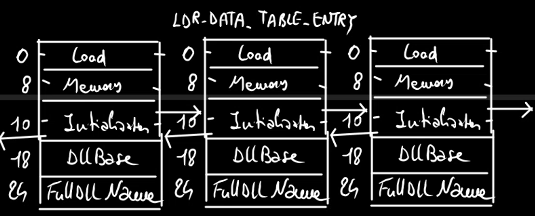
\includegraphics[scale=0.5]{immagini/ldr_struct.png}
\end{figure}
e questo vale per tutte e 3 le strutture dati.\\Il motivo fondamentale per questa cosa è efficienza: non conoscendo a priori la dimensione della struttura, andando ogni volta all'inizio sporcherei più linee di cache, facendo così invece si dimezzano le linee di cache usate. Quindi, sommerò gli offset in base alla posizione del campo, che è a 10h e non sapendolo il codice risulterebbe "misterioso".
\subsection{Trovare l'indirizzo della DLL}
Lo shellcode ora ha trovato l'indirizzo di base della DLL e quindi può cercare l'indirizzo della API, che si trova nella testata PE della DLL, che ha la sezione "Exports", dobbiamo rifare a mano il lavoro della \texttt{GetProcAddress}. Per farlo, dobbiamo capire come è organizzata la sezione "Exports": proviamo ad aprire con PE-Bear un qualunque eseguibile, cerchiamo poi la dll \texttt{kernelbase}:
\begin{itemize}
	\item all'inizio, abbiamo una serie di testa non importanti, ma all'offset 3ch c'è l'RVA (Relative Virtual Address) dell'inizio della testata successiva, che è l'offset rispetto all'indirizzo dove è stata caricata la DLL.\\L'RVA in linea di principio è diverso volta per volta, quindi lo shellcode deve come prima cosa trovare l'RVA ed aggiungerlo alla DLL base
	\item quindi, da [[Base + c3] + Base] otteniamo l'indirizzo di base delle testate PE.\\Arrivato qui, ci sono
	\begin{itemize}
		\item 2 byte di signature
		\item una IMAGE\_FILE\_HEADER, lunga 18-22 byte
		\item abbiamo poi la OPTIONAL\_HEADER, di cui ci importa l'RVA della Export Directory.
	\end{itemize}
	Quindi, preso questo RVA e sommato all'indirizzo di base in cui è caricata la DLL si ottiene la tabella degli exports della DLL
	\item A questo punto, lo shellcode deve interpretare a mano la tabella degli Exports
\end{itemize}
Sommando quindi IMAGE\_FILE\_HEADER + OPTIONAL = Export Directory, la somma di tutti i byte è 120. Quindi [[Base + c3] + Base] + 120 ci da l'RVA della Export Directory, ma ora occorre l'indirizzo della Export Directory.
\subsubsection{Export Directory}
La Export Directory è fatta da diversi campi: innanzitutto c'è una struttura di dati dove:
\begin{itemize}
	\item ad offset 18h c'è il campo \texttt{NumberOfNames}
	\item ad offset 1ch c'è \texttt{NumberOfFunction}
	\item a 20h \texttt{AddressOfFunctions}
	\item a 20h \texttt{AddressOfNames}, l'RVA di un vettore di puntatori a stringhe. Queste stringhe, descrivono le varie API esportate. Il vettore è ordinato alfabeticamente, quindi tipicamente sapendo il numero di nomi, l'ordine e sapendo cosa cercare si fa una ricerca binaria, ma nessuno shellcode lo fa;
	\item a 24h \texttt{AddressOfNamesOrdinals}, ordinata per numero d'ordine. Sono comunque valori a 16 bit e serve perché \texttt{AddressOfFunctions} elenca gli RVA delle funzioni per ordinale, quindi comincia dall'ordinale 1 e va avanti.\\Dopo di che, è \texttt{AddressOfNamesOrdinals} a fare il collegamento fra nome e numero d'ordine: se ad indice 100 trovo un nome, trovo in questo vettore l'ordinale da usare nel vettore \texttt{AddressOfFunctions}
\end{itemize}
Arriviamo quindi ad avere idealmente \texttt{LoadLibraryA} e \texttt{GetProcAddress} ma in realtà non serve: una delle cose non documentate di Microsoft è che la \texttt{LoadLibraryA} restituisce un handle che coincide con la DLLbase a cui è caricata la dll, quindi non serve usare la \texttt{GetProcAddress} in quanto possiamo usare questa base e navigare verso quello che serve.
\subsection{Ottimizzazioni degli shellcode}
Quando si cerca effettivamente la DLL, come si fa? E stesso vale per la API da cercare, si dovrebbe usare una stringa nel codice ed usare strcmp, ma questo non va bene perché:
\begin{enumerate}
	\item le stringhe occupano spazio
	\item le stringhe sono trovabili
\end{enumerate}
quindi lo shellcode piuttosto usa un hash: abbiamo una funzione \textbf{hashString:} gli passiamo la stringa della API voluta e questa tira fuori un hash di 32 bit. Si mette quindi l'hash corrispondente alla stringa, verifica il matching con il nome e se trova quello che cerca si ferma. Questo viene fatto per offuscare il codice ed inoltre la funzione di hash non deve essere molto complessa, basta che non produca collisioni fra le API usate dallo shellcode.\\Tipicamente, molti shellcode usano funzioni di hash tirate fuori da metasploit, che è basato su una rotazione dei bit di un carattere di 13 posizioni, per poi sommare il risultato ad un accumulatore.\\\\Seconda ottimizzazione: spesso lo shellcode non si preoccupa di cercare esplicitamente di cercare la kernel32.dll, perché assumono spesso che sia la 2° dll caricata, in quanto la prima è ntdll.dll. Nelle ultime versioni di Windows non è sempre garantito, ma molto spesso funziona, altrimenti si usa l'hash come sopra.
\section{Esempio}
L'esempio, visto dall'ASM, invoca findKernel32Base che fa esattamente ciò che abbiamo detto prima:
\begin{itemize}
	\item parte da fs + 0x30 per trovare la TEB
	\item testa il risultato, perché la TEB nelle vecchie versioni di Windows stava in memoria alta (oltre il 3° GB), mentre ora sta in memoria bassa. Quindi lo shellcode non vuole funzionare su Windows non recenti
	\item eax punta la TEB, si dereferenzia per arrivare alla 3° lista
	\item la lodsb prende l'indirizzo  a cui punta esi e lo carica in eax: esi punta alla struttura degli Init stessi e quindi ora eax punta alla locazione successiva, ovvero al 2° elemento della lista
	\item somma quindi 8 a cosa ha ottenuto per arrivare a DllBase
	\item cerca poi, con la findSymbolByHash, il simbolo nella DLL confrontando con l'hash appena caricato sullo stack
	\item dalla base +3c ottiene l'RVA della testata, somma poi 120 alla base ed arriva all'indirizzo che contiene l'indirizzo della Export Directory.
	\item sommiamo alla base per trovare l'indirizzo, dereferenziamo e troviamo i numeri \texttt{NumberOfNames} ed \texttt{AddressOfNames}
	\item in un loop, dereferenzia il puntatore, calcola l'hash e confronta con l'hash della funzione da cercare
	\item ora fa tutti i passaggi rimanenti per poi restituire l'indirizzo della funzione cercata
\end{itemize}
A questo punto, costruisce i parametri ed invoca la funzione.
\section{Operazioni sugli shellcode}
Ci sono due operazioni che si fanno sugli shellcode:
\begin{enumerate}
	\item avere shellcode codificati con caratteri stampabili, \textbf{shellcode encoding}: questo perché si vorrebbero usare funzioni come \texttt{strcat}, \texttt{strcmp} etc... così magari da sfruttare vulnerabilità di buffer overflow.\\È importante che sia fatto da caratteri stampabili in quanto spesso ci sono delle funzioni che verificano la stampabilità dei caratteri prima di passarli alle funzioni.\\Abbiamo quindi una piccola parte dello shellcode che è il decoder e poi una lunga parte che è lo shellcode encoded: la codifica prevede che ogni byte dello shellcode sia fatto in realtà da 2 byte: abbiamo la base della lettera 'A' + un valore da 0 a 15, quindi ogni carattere è sempre stampabile.\\La sequenza AB rappresenta quindi 0x01, mentre BA rappresenta 0x10. Il decoder prende la lista di caratteri stampabili e costruisce il vero shellcode, per poi saltarci dentro.\\Il decoder stesso non deve contenere caratteri non stampabili, ma essendo piccolo è fattibile
	\item \textbf{NOP sleds}: lo shellcode è fatto di 3 parti: shellcode, decoder e byte di padding che rappresentano NOP. Spesso si usa 0x90 ma non è stampabile (perché maggiore di 128), quindi si usano delle istruzioni NOP nel range sotto 128, magari non tutte uguali per non essere scoperti. Si possono magari usare byte nel range 0x40 - 0x4f, che magari fanno inc eax inutili.\\Si usa perché spesso le tecniche che iniettano shellcode non hanno modo di controllare il punto in cui il processore salterà, perché vanno riscritti fondamentalmente degli indirizzi di ritorno dello stack. IN questo modo, saltando in un qualunque punto del padding si arriverà sul decoder e si salterà dentro allo shellcode decodificato
\end{enumerate}
L'obiettivo è sempre quello di riconoscere cosa analizziamo.

\newpage
\chapter*{Appendice}
\section*{Comandi utili per Ghidra}
\begin{itemize}
\item con il tasto "G" si apre il box per saltare in un certo punto del file, dando un'etichetta o un indirizzo esadecimale;
\item passando su un valore esadecimale, è possibile passarvi sopra per vedere il valore. Col tasto destro si può convertire il valore;
\item è possibile richiedere un call graph, che rappresenta con ogni punto una funzione e rappresenta tutte le call che la funzione fa. Rispetto ad IDA; Ghidra riesce a mostrare le call solo per il livello successivo del grafo, poi bisognerebbe andare avanti a mano;
\item symbol tree definisce tutti i simboli usati da Ghidra, come anche tutti i simboli che sono stati riconosciuti come funzioni;
\item con "X" si trovano tutti i riferimenti ad una chiamata di funzione;
\item ";" permette di inserire i commenti, in quanto in assembly si fa così;
\item tasto dx sulla funzione $\rightarrow$ edit stack frame: permette di modificare le variabili sullo stack, ad esempio aggiungendone il tipo
\item memory map: finestra che elenca tutti i "segmenti" di memoria su cui Ghidra ha costruito il reversing. Importante in quanto ogni tanto è necessario far capire a Ghidra come è fatto un certo segmento, da un quadro di insieme della struttura dell'eseguibile
\item per aprire i riferimenti a variabili, tasto dx sul simbolo per andare sui riferimenti. vengono mostrati riferimenti al simbolo o all'indirizzo, vogliamo generalmente quelli all'indirizzo, c'è la scorciatoia con "X". Questa funzionalità si usa di continuo.
\item menù di ricerca, si può cercare sia nelle istruzioni macchina che nella memoria. Fondamentalmente, quello sulla memoria è più generale, ci sono poi sotto-menù che fanno ricerche a grana più fine
\end{itemize}
\end{document}